%%%%%%%%%%%%%%%%%%%% book.tex %%%%%%%%%%%%%%%%%%%%%%%%%%%%%
%
% sample root file for the chapters of your "monograph"
%
% Use this file as a template for your own input.
%
%%%%%%%%%%%%%%%% Springer-Verlag %%%%%%%%%%%%%%%%%%%%%%%%%%


% RECOMMENDED %%%%%%%%%%%%%%%%%%%%%%%%%%%%%%%%%%%%%%%%%%%%%%%%%%%
\documentclass[graybox,envcountchap,sectrefs]{svmono}

% choose options for [] as required from the list
% in the Reference Guide
\hyphenation{op-tical net-works wire-less semi-conduc-tor primary intro-duction un-licensed acc-ess avail-able}

\usepackage{mathptmx}
\usepackage{helvet}
\usepackage{courier}
%
\usepackage{type1cm}         
\usepackage{placeins}
\usepackage{makeidx}         % allows index generation
\usepackage{graphicx}        % standard LaTeX graphics tool
                             % when including figure files
\usepackage{multicol}        % used for the two-column index
\usepackage[bottom]{footmisc}% places footnotes at page bottom

\usepackage{mathtools,amsfonts,amssymb}
\usepackage{xfrac}
\usepackage{algpseudocode}
\usepackage{algorithm}
\usepackage[caption=false,font=footnotesize]{subfig}
% see the list of further useful packages
% in the Reference Guide

\makeindex             % used for the subject index
                       % please use the style svind.ist with
                       % your makeindex program

%%%%%%%%%%%%%%%%%%%%%%%%%%%%%%%%%%%%%%%%%%%%%%%%%%%%%%%%%%%%%%%%%%%%%

\begin{document}
\author{Quang-Dung Ho, Daniel Tweed, \mbox{Tho Le-Ngoc}}
\title{Long Term Evolution (LTE) in Unlicensed Bands}
%\textbf{}\subtitle{-- Monograph --}
\maketitle

\frontmatter%%%%%%%%%%%%%%%%%%%%%%%%%%%%%%%%%%%%%%%%%%%%%%%%%%%%%%

%
%%%%%%%%%%%%%%%%%%%%%%% dedic.tex %%%%%%%%%%%%%%%%%%%%%%%%%%%%%%%%%
%
% sample dedication
%
% Use this file as a template for your own input.
%
%%%%%%%%%%%%%%%%%%%%%%%% Springer %%%%%%%%%%%%%%%%%%%%%%%%%%

%TODO: Write dedication, if that is desired 
\begin{dedication}
This work is dedicated to Claude Shannon and Alan Turing, without whom none of us would have an interest in this subject, and to our families, without whom none of us would be able to dedicate our time to research.
\end{dedication}
%%%%%%%%%%%%%%%%%%%%%%%foreword.tex%%%%%%%%%%%%%%%%%%%%%%%%%%%%%%%%%
% sample foreword
%
% Use this file as a template for your own input.
%
%%%%%%%%%%%%%%%%%%%%%%%% Springer %%%%%%%%%%%%%%%%%%%%%%%%%%

\foreword

%% Please have the foreword written here
Use the template \textit{foreword.tex} together with the Springer document class SVMono (monograph-type books) or SVMult (edited books) to style your foreword\index{foreword} in the Springer layout. 

The foreword covers introductory remarks preceding the text of a book that are written by a \textit{person other than the author or editor} of the book. If applicable, the foreword precedes the preface which is written by the author or editor of the book.


\vspace{\baselineskip}
\begin{flushright}\noindent
Place, month year\hfill {\it Firstname  Surname}\\
\end{flushright}




%%%%%%%%%%%%%%%%%%%%%%preface.tex%%%%%%%%%%%%%%%%%%%%%%%%%%%%%%%%%%%%%%%%%
% sample preface
%
% Use this file as a template for your own input.
%
%%%%%%%%%%%%%%%%%%%%%%%% Springer %%%%%%%%%%%%%%%%%%%%%%%%%%

\preface

Global mobile traffic is expected to increase nearly tenfold by 2020 due to the increasing number of mobile-connected devices and the explosion of data-hungry mobile applications. Pushing traffic towards the network capacity quickly deteriorates the Quality of Service (QoS) perceived by users. Acquiring additional licensed spectrum to increase the capacity of Radio Access Networks (RANs) is certainly very expensive. Mobile operators are also challenged by the “revenue gap”, i.e. the exponential increase in mobile traffic does not generate sufficient additional revenues required for upgrading their RANs. These circumstances has fostered an interest in cost-effective solutions to increase the capacity of RANs. Long-Term Evolution (LTE) in unlicensed bands (U-LTE) is among promising solutions. However, since U-LTE is a nascent LTE technology, there are still various associated concerns and challenges to be addressed.

This brief first presents a comprehensive survey on U-LTE, focusing on technical issues and the impacts of this technology to other neighboring networks in shared frequency bands. Specifically, the concepts, motivations, benefits, obstacles, and coexistence requirements of U-LTE are presented. Three typical types of U-LTE, including LTE-U, LAA-LTE, and MuLTEfire are explained. Next, regulations specified by standard institutes for radio systems operating in unlicensed spectrum are reviewed. Due to the fact that technical knowledge of the medium access mechanisms of LTE and IEEE 802.11/Wi-Fi technologies is strongly required to understand and analyze the interactions between these two technologies when they operate in the same frequency band, high-level network architectures and technical details of LTE and Wi-Fi are presented. Especially, distinguishing features of CSMA/CA employed by Wi-Fi networks compared to standardized regulations are highlighted. Forth, in order to capture the ongoing activities on U-LTE’s coexistence mechanisms, related works are surveyed with insight observations on their limitations and concerns. 

This brief also presents our Network-Aware Adaptive LBT mechanism (NALT) which is proposed for LTE coexistence with Wi-Fi networks. In a nutshell, NALT monitors both channel conditions and usage activity to maximize its transmission opportunities, while maintaining fair sharing of the channel, in a way that is transparent to incumbent Wi-Fi devices. Finally, towards future working directions, in the light of the survey, this brief identifies a number of open technical questions as well as related potential research issues in U-LTE.

The findings in this brief provide telecom engineers, researchers, and academic professionals with valuable knowledge and potential working or research directions when designing and developing medium access protocols for next generation wireless access networks.

This work was partially supported by the Natural Sciences and Engineering Research Council (NSERC) through an NSERC CRD Grant with Huawei Technologies Canada.

\vspace{\baselineskip}
\begin{flushright}\noindent
Montreal, Canada,\hfill {\it Quang-Dung Ho}\\
September 2016\hfill {\it Daniel Tweed}\\
\hfill {\it Tho Le-Ngoc}\\
\end{flushright}
%%%%%%%%%%%%%%%%%%%%%%%acknow.tex%%%%%%%%%%%%%%%%%%%%%%%%%%%%%%%%%%%%%%%%%
% sample acknowledgement chapter
%
% Use this file as a template for your own input.
%
%%%%%%%%%%%%%%%%%%%%%%%% Springer %%%%%%%%%%%%%%%%%%%%%%%%%%

\extrachap{Acknowledgements}

Use the template \emph{acknow.tex} together with the Springer document class SVMono (monograph-type books) or SVMult (edited books) if you prefer to set your acknowledgement section as a separate chapter instead of including it as last part of your preface.


%
\tableofcontents
%
%%%%%%%%%%%%%%%%%%%%%%acronym.tex%%%%%%%%%%%%%%%%%%%%%%%%%%%%%%%%%%%%%%%%%
% sample list of acronyms
%
% Use this file as a template for your own input.
%
%%%%%%%%%%%%%%%%%%%%%%%% Springer %%%%%%%%%%%%%%%%%%%%%%%%%%

\extrachap{Acronyms}
%TODO: Compile list of Acronyms
\begin{description}[CABR]
\item[ABC]{Spelled-out abbreviation and definition}
\item[BABI]{Spelled-out abbreviation and definition}
\item[CABR]{Spelled-out abbreviation and definition}
\end{description}

\mainmatter%%%%%%%%%%%%%%%%%%%%%%%%%%%%%%%%%%%%%%%%%%%%%%%%%%%%%%%
%%%%%%%%%%%%%%%%%%%%%%part.tex%%%%%%%%%%%%%%%%%%%%%%%%%%%%%%%%%%
% 
% sample part title
%
% Use this file as a template for your own input.
%
%%%%%%%%%%%%%%%%%%%%%%%% Springer %%%%%%%%%%%%%%%%%%%%%%%%%%

\begin{partbacktext}
\part{Part Title}
\noindent Use the template \emph{part.tex} together with the Springer document class SVMono (monograph-type books) or SVMult (edited books) to style your part title page and, if desired, a short introductory text (maximum one page) on its verso page in the Springer layout.

\end{partbacktext}
%%%%%%%%%%%%%%%%%%%%% chapter.tex %%%%%%%%%%%%%%%%%%%%%%%%%%%%%%%%%
%
% sample chapter
%
% Use this file as a template for your own input.
%
%%%%%%%%%%%%%%%%%%%%%%%% Springer-Verlag %%%%%%%%%%%%%%%%%%%%%%%%%%
%\motto{Use the template \emph{chapter.tex} to style the various elements of your chapter content.}
\chapter{Introduction}
\label{intro} 

\abstract*{The increasing penetration of mobile-connected devices and the emergence of numerous data-hungry mobile applications has created a wide range of business opportunities for mobile network operators and service providers. Meanwhile, this growth is placing a greater pressure on the capacity that the Radio Access Networks (RANs) have to provide. This chapter begins with a review of technical challenges that motivate developments of cost-effective solutions to improve the capacity of RANs. The technology which utilizes the unlicensed frequency bands in Long-Term Evolution (LTE), namely U-LTE, is singled out as the most promising solution. Benefits and obstacles of this technology are then presented. Next, three typical forms of U-LTE including LTE-U, LAA-LTE, and MulteFire are explained. Concerns on the interactions between U-LTE and Wi-Fi in radio channel access and their coexistence are discussed in detail. Finally, key requirements for the coexistence of U-LTE and Wi-Fi are summarized.}  

The increasing penetration of mobile-connected devices and the emergence of numerous data-hungry mobile applications has created a wide range of business opportunities for mobile network operators and service providers. Meanwhile, this growth is placing a greater pressure on the capacity that the Radio Access Networks (RANs) have to provide. This chapter begins with a review of technical challenges that motivate developments of cost-effective solutions to improve the capacity of RANs. The technology which utilizes the unlicensed frequency bands in Long-Term Evolution (LTE), namely U-LTE, is singled out as the most promising solution. Benefits and obstacles of this technology are then presented. Next, three typical forms of U-LTE including LTE-U, LAA-LTE, and MulteFire are explained. Concerns on the interactions between U-LTE and Wi-Fi in radio channel access and their coexistence are discussed in detail. Finally, key requirements for the coexistence of U-LTE and Wi-Fi are summarized.


\section{Motivations and Concepts of U-LTE}
\label{lte-motiv}

Global mobile traffic is expected to increase nearly tenfold between 2014 and 2020 due to the increasing number of mobile-connected devices and the explosion of data-hungry mobile applications \cite{cisco_mobile_traffic_2015}. The expected growth in traffic is shown in detail in Fig. \ref{figs:global-mobile-data-traffic-2015-2020}, where the $3.7$ exabytes per month seen in 2015 is forecast to grown at a compound annual growth rate of 53\%, reaching $30.6$ exabytes per month by 2020. 
\begin{figure}[!ht]
	\centering
	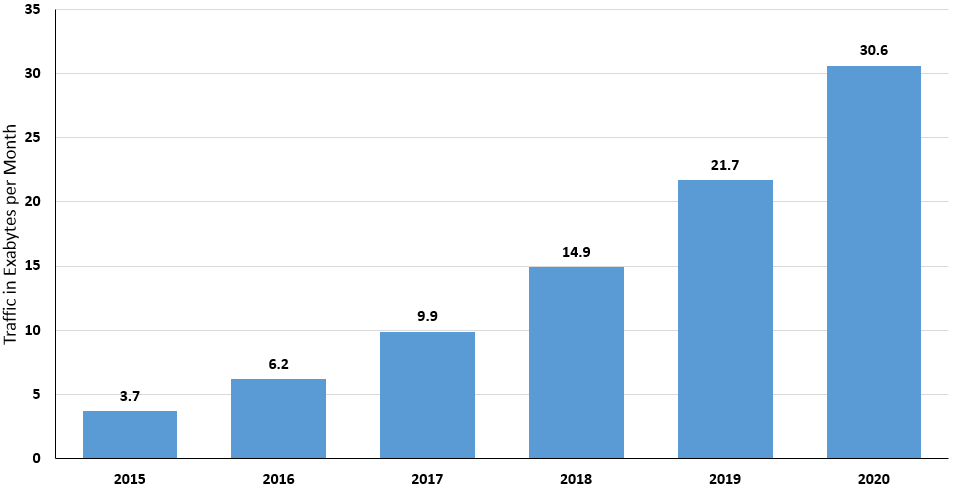
\includegraphics[width=\textwidth]{figs/global-mobile-data-traffic-2015-2020}
	\caption{Global mobile data traffic from 2015-2020 \cite{cisco_mobile_traffic_2015}.}
	\label{figs:global-mobile-data-traffic-2015-2020}
\end{figure}
Pushing traffic towards the network capacity quickly deteriorates the Quality of Service (QoS) perceived by the users. As a result, increasing the capacity of their Radio Access Network (RAN) is one of the top-priority action plans of mobile service providers. Purchasing additional licensed spectrum is a straight-forward solution to this but radio spectrum is very much limited and increasingly expensive. Furthermore, mobile operators are at the same time challenged by the ``revenue gap'', i.e., the exponential increase in mobile traffic does not generate sufficient additional revenues which would be required for upgrading their RANs. This circumstance has fostered interest in cost-effective solutions to increase RAN capacity. Mobile data off-loading and Long-Term Evolution (LTE) in unlicensed bands (U-LTE) are among the most promising solutions.

Mobile data offloading is the use of a complementary wireless technology to transport data originally flowing through the cellular mobile network. Wi-Fi offloading and Device-to-Device (D2D) communications are the two main data offload techniques. Rules determining when and how the mobile offloading actions are triggered are set by either mobile subscribers or network operators. For the subscribers, data offloading helps them to exploit the availability of higher bandwidth data service at lower costs. For the operators, the most obvious benefit of this kind of approach is the mitigation of cellular mobile network load and thus congestion. Besides, shifting data to a complementary wireless technology leads to a number of other improvements including an overall increase in network throughput, a reduction of content delivery time, the extension of network coverage and increase of network availability, and better energy efficiency. Unfortunately, these benefits come with a number of challenges related to infrastructure coordination, network/technology hand-overs, service continuity, pricing, business models, and lack of existing standards. 

Recently, U-LTE has appeared as the most promising approach to enhance RAN capacity and address the revenue gap in mobile networks. The original idea of LTE-U is fairly straightforward: By definition, it is an LTE technology that puts cellular signals into the unlicensed spectrum with the support of existing LTE features including Supplemental Downlink (SDL, proposed in LTE Release 9 and later) and Carrier Aggregation (CA, proposed in LTE Release 10 and later).  As mentioned, mobile operators are facing a great pressure on capacity and cost. If LTE can exploit the unlicensed band (where IEEE 802.11/Wi-Fi and other radio systems are using), then it will obtain a considerable additional capacity at a minimal cost. U-LTE can be used to boost downlink or both uplink and downlink of LTE networks, as illustrated in Fig. \ref{figs:U-LTE-use_model}.
\begin{figure}[!ht]
	\centering
	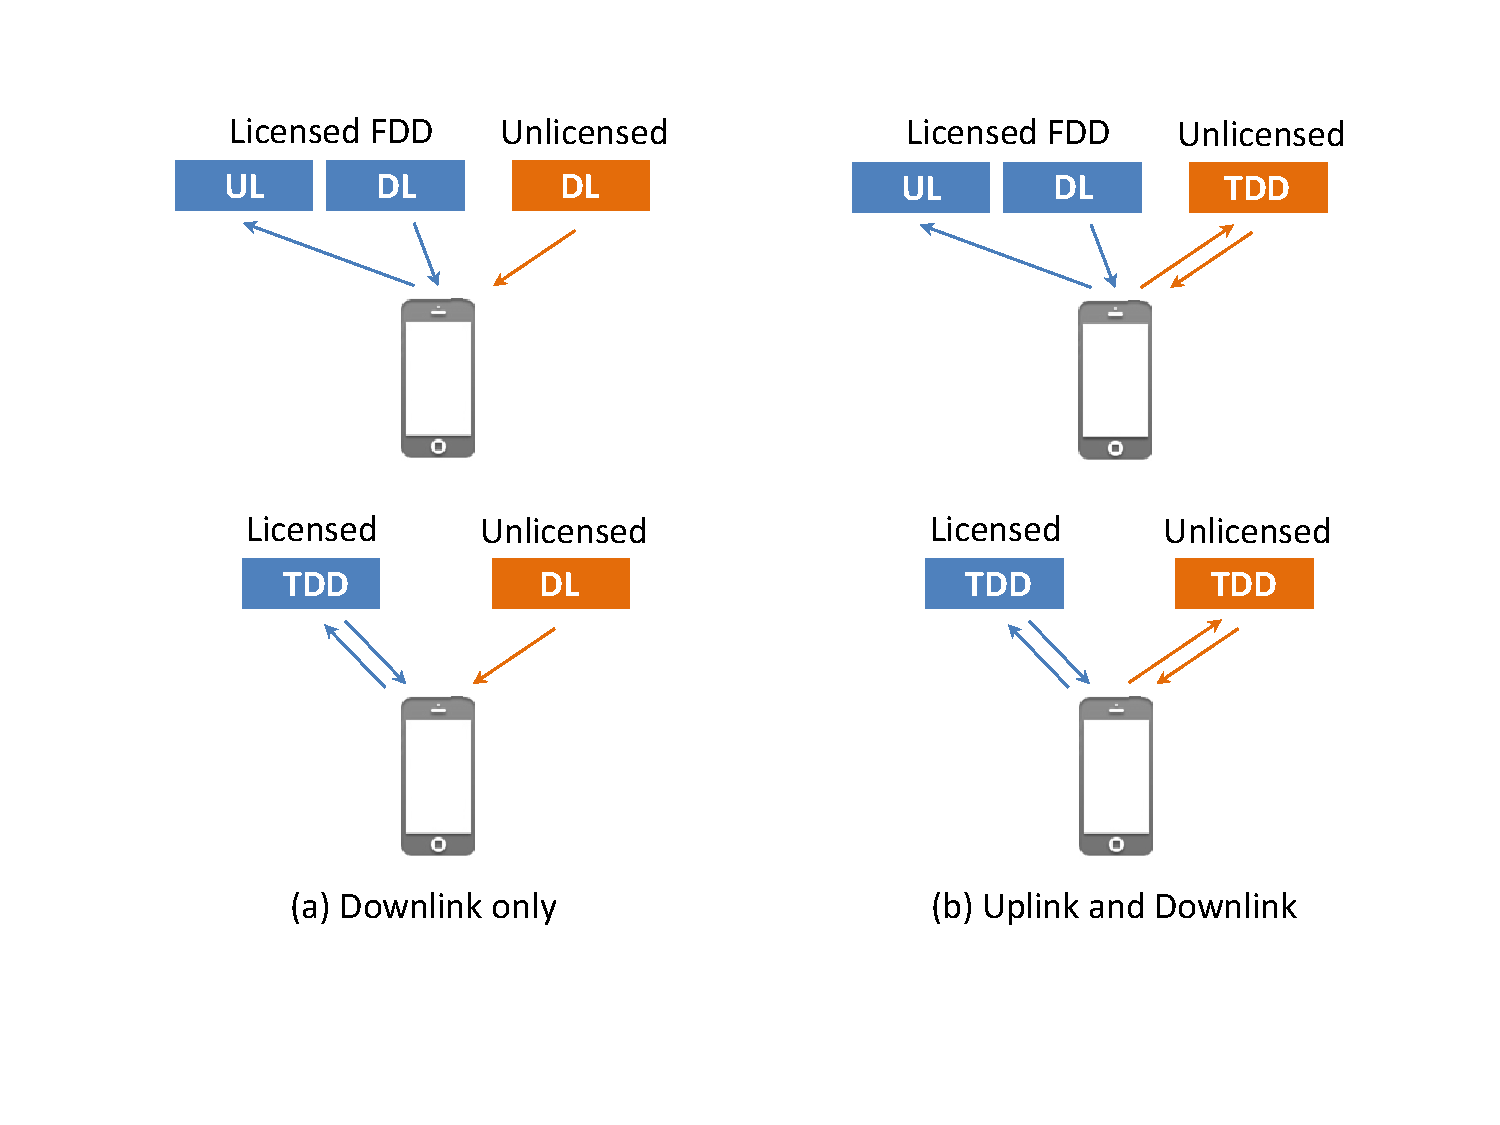
\includegraphics[width=0.75\textwidth]{figs/U-LTE-use_model}
	\caption{Use cases of U-LTE.}
	\label{figs:U-LTE-use_model}
\end{figure}

Historically, U-LTE was originally proposed and officially announced by Qualcomm in 2013 \cite{Qualcomm-U-LTE-2013}. Currently, it focuses on $500$ MHz of spectrum available in the $5$ GHz band. Specifically, according to the proposal from Qualcomm, U-LTE is to use the U-NII-3 part of the $5$ GHz band, which has highest allowed Equivalent Isotropically Radiated Power (EIRP). While in the $2.4$ GHz band, regulatory bodies limit EIRP to $100$ mW (in Europe) or $200$ mW (in United States), the U-NII-3 enjoys the rights to go as high as $1000$ mW outdoors.

\section{Benefits and Obstacles of U-LTE}
\label{lte-ben}
U-LTE is expected to offer numerous benefits to mobile network operators, service providers, and consumers. Free access to the unlicensed spectrum provides additional capacity to the network at a minimal cost compared to purchasing licensed spectrum allocations. Therefore, U-LTE appears to be a very inexpensive way to meet the future traffic growth. U-LTE will give operators the option to make use of unlicensed spectrum within a unified network, offering potential operational cost savings, improving spectral efficiency, and providing a better user experience. Compared to the Wi-Fi offloading technology, U-LTE has the potential to offer significantly better coverage and higher spectral efficiency while allowing seamless flow of data across licensed and unlicensed channels in a single core network. U-LTE could also take advantage of the robust security features which are already in place in LTE networks, rather than relying on external or complementary networks. Finally, Wi-Fi offloading leads to less traffic on mobile networks and thus may result in revenue losses in data services.  Since U-LTE could be managed through a single core network, it could provide an incremental ability for mobile service providers to directly bill for data usage.

Despite the obvious benefits of U-LTE, there are a number of substantial obstacles. First, even though U-LTE is not charged for the use of unlicensed spectrum, compared to Wi-Fi, its network deployment could be more expensive. The LTE chipset itself is several times more expensive than that of Wi-Fi (a few tens of dollars compared to a few dollars or less than one dollar). LTE base stations and other network devices are likely to cost substantially more than the required Wi-Fi access points to service the same area in the unlicensed bands.  Also, LTE operators need to deploy and maintain expensive back-haul links between base stations and from the base station to the core network. Being an LTE technology, U-LTE will work only with LTE-capable devices while there have been many more devices that feature Wi-Fi connectivity than LTE. Wi-Fi is nearly always integrated into laptops, tablets, cameras, and other connected consumer devices. Additionally, from technical perspectives, the premium features provided by U-LTE (e.g., seamless voice and data roaming) may not prove sufficiently more valuable than those offered by emerging Wi-Fi technologies such as Hotspot 2.0, so-called Wi-Fi Certified Passpoint, which is a new standard for public-access Wi-Fi that enables seamless roaming among Wi-Fi networks and between Wi-Fi and cellular networks. Finally, the biggest challenge of U-LTE is its coexistence with other radio networks operating in the same frequency bands. 

\section{Three Types of U-LTE}
\label{lte-types}
There are three different flavors of U-LTE currently under development: LTE unlicensed (LTE-U), Licensed Assisted Access LTE (LAA-LTE), and MulteFire. The first two flavors require ``anchoring licensed spectrum'', i.e., they operate primarily in licensed spectrum and opportunistically exploit access to the unlicensed spectrum for an additional bandwidth boost. Devices are still anchored in licensed spectrum for LTE management/control signaling and high QoS data while using the unlicensed spectrum for only best-effort or delay-tolerant data. The third flavor is developed by Qualcomm and requires no licensed spectrum at all, therefore, it is often referred to as stand-alone U-LTE. MulteFire is designed for indoor use and deployments by enterprises, cable companies and other service providers without ownership of expensive bandwidth licenses. However, at the present time, there are very few technical details available about MulteFire.


\subsection{LTE-U}
LTE-U is the simplest form of U-LTE and requires only minor modifications in LTE protocol stack. Therefore, it can quickly facilitate pre-standard equipment manufacturing and deployment. LTE-U first attempts to select a clear channel to access. If no clear channel is found, it will employ Carrier-Sensing Adaptive Transmission (CSAT), which is a Time-Division Multiplex (TDM) coexistence mechanism based on medium sensing. The CSAT mechanism is depicted in in Fig. \ref{figs:LTE-U}.
\begin{figure}[!ht]
	\centering
	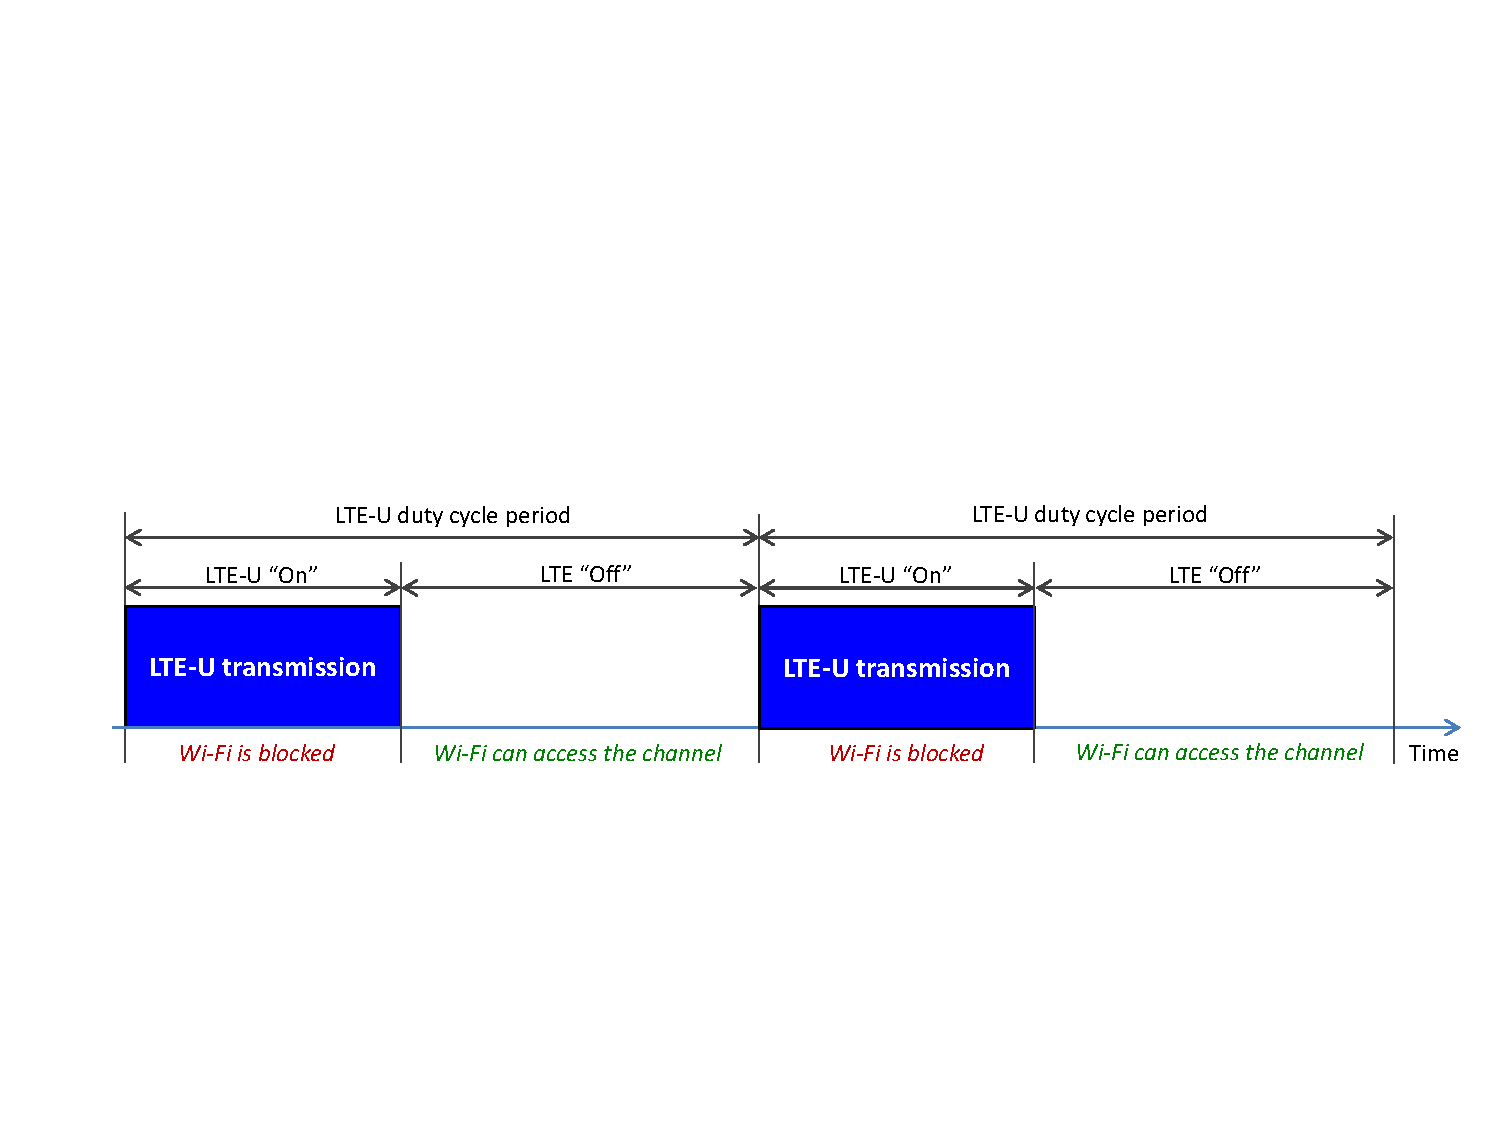
\includegraphics[width=\textwidth]{figs/LTE-U}
	\caption{Duty-cycling mechanism employed by LTE-U.}
	\label{figs:LTE-U}
\end{figure}
CSAT employs duty-cycling, which enforces the TDM cycle on other users of the channel, instead of LBT mechanism.  In particular, CSAT defines a time cycle where the base station transmits in a fraction of the cycle and then gates off in the remaining duration. Compared to LBT or CSMA, the base station senses the medium for a longer duration (around $10$s of milliseconds to $200$ milliseconds) and according to the observed medium activities the algorithm gates off LTE transmission proportionally.  The duty cycle of transmission versus gating off is dictated by the sensed medium activity of neighboring RANs. The TDM cycle can be set to a few tens or hundreds of millisecond, which can effectively accommodate the activation/de-activation procedures while controlling the data transmission delay. An important observation from Fig. \ref{figs:LTE-U} is that during the LTE ``on'' period, Wi-Fi is blocked by LTE-U transmissions. During the LTE ``off'' period, Wi-Fi will detect that the channel is free and can schedule its transmissions following its CSMA-CA protocol.

LTE-U is only applicable in areas where there are no strict LBT requirements for operations in unlicensed bands (e.g., US, Korea, and China). It is a non-standard version of U-LTE, being developed outside of the 3GPP standards process. LTE-U is supported by the LTE-U Forum formed in 2014 by Verizon in cooperation with Alcatel-Lucent, Ericsson, Qualcomm Technologies Inc. (a subsidiary of Qualcomm Incorporated), and Samsung.

\subsection{LAA-LTE}
In many regions (e.g., Europe, Japan, and India) there exist regulations for accessing the unlicensed spectrum that require equipment to periodically check for the presence of other occupants in the channel, so-called LBT. LAA-LTE is designed for use in such areas, but also for global use. It requires a number of modifications so that LTE transmissions can meet regulatory requirements in LBT regions. Similar to LTE-U, LAA-LTE first tries to choose the cleanest channel available, based on Wi-Fi and LTE measurements. In the event that no clean channel is available, a LBT algorithm is used to compete for the medium with other RANs. For LBT, different mechanisms for frame-based equipment (FBE) and load-based equipment (LBE) have been specified in \cite{LBT-ETSI-2014}. Details of these types of the devices and the applicable mechanisms are presented in Chapter \ref{sec:LBT-overview}.

Assuming that LBE LBT is employed for LAA-LTE, before transmission, a clear channel assessment  (CCA) using and energy detect (ED) threshold is performed. If the channel is clear during a CCA slot ($20$ microseconds or longer), transmission is started immediately. Otherwise, and extended CCA (ECCA) is performed. If the channel is clear during $N$ CCA slots, transmission is started immediately where $N$ is a random integer uniformly distributed from $1$ to $q$, and $q \in \{4,5,...,32\}$ is a pre-determined constant. The total time to occupy the channel without CCA is limited to $(13/32)q$ milliseconds (e.g., $13$ milliseconds when $q$ is $32$). Two simplified scenarios with LAA-LTE (employing LBE-based LBT) and Wi-Fi systems operating in the same channel are illustrated in Fig. \ref{figs:LAA-LTE}. 
\begin{figure}[!ht]
	\centering
	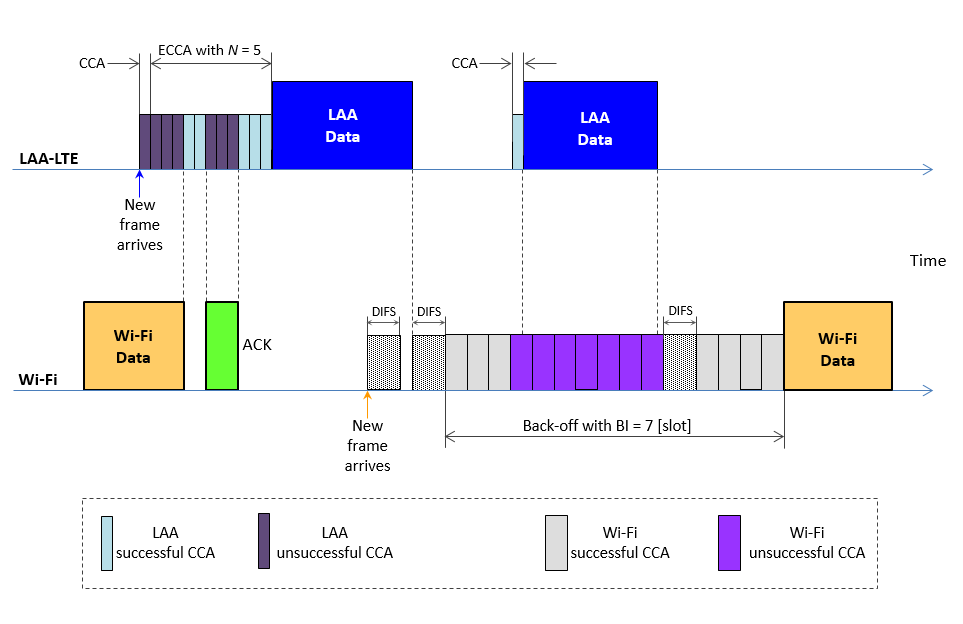
\includegraphics[width=0.9\columnwidth]{figs/LAA-LTE}
	\caption{CCA and ECCA mechanisms employed by LAA-LTE.}
	\label{figs:LAA-LTE}
\end{figure}
In the first scenario, the LAA-LTE system, upon having data frames to send, performs CCA and then ECCA (with $N=7$) since there is an ongoing Wi-Fi transmission. The ECCA procedure is frozen and then resumed when another Wi-Fi transmission takes place and then completes, respectively. The LAA-LTE system finally transmits its frames once its ECCA counter reaches zero. In the second scenario, the Wi-Fi system, upon having data frames to send, performs CCA and then back-off procedure (with $\mathrm{BI_{slots}} = 7$) since there is an ongoing LAA-LTE transmission. The back-off procedure is frozen and resumed when another LAA-LTE transmission takes place. The Wi-Fi system finally transmits its frames once back-off counter reaches zero.

Since LTE was originally designed for licensed spectrum and a centralized management (i.e., network-controlled) model, it is generally an ``always-on'' technology. As a result, adapting to LBT is a marked change for the LTE protocol. Compared to LTE-U, which is downlink-only in the unlicensed bands, LAA-LTE may be used to support bi-directional traffic in unlicensed bands. LAA-LTE is currently actively supported by 3GPP and is included in 3GPP LTE Release 13. T-Mobile USA and Verizon Wireless have indicated their interests in deploying pre-standard LAA-LTE systems for evaluations and commercial services in 2016.



\subsection{MulteFire}
At this time there are very few technical details available about MulteFire. It is unknown which MAC protocols or coexistence mechanisms are employed in this type of U-LTE. Also, since licensed frequency is not used for LTE network management and control signaling, as opposed to the conventional LTE and the other two variants of U-LTE (i.e., LTE-U and LAA-LTE) that are license anchored, MulteFire may lose all advantages of native LTE technologies. It is expected that MulteFire will be less efficient than LTE-U and LAA-LTE and therefore its achievable performance/efficiency may be just marginally better than that of Wi-Fi. Then the question on the applicability of MulteFire needs to be answered.


\section{Coexistence of U-LTE and Wi-Fi}
\label{coexist}
It is well known that multiple radio communications technologies operating in a common frequency band will negatively affect each other if respectful coexistence mechanisms are not employed. As a result, despite the fact that U-LTE can offer various benefits, its coexistence with Wi-Fi and other radio systems that operate in the $5$ GHz frequency band is the biggest concern. In specific, it is believed that U-LTE may considerably interfere with Wi-Fi systems and/or grasp more radio resources when they operate in the same frequency band due to the following:
\begin{itemize}
\item \textit{First}, LTE was originally designed to work in its own licensed frequency band rather than to coexist with other radio access technologies in a shared band. LTE employs Orthogonal Frequency-Division Multiple Access (OFDMA) and transmits almost continuously without requiring or implementing any mechanism for spectrum sharing. Wi-Fi, on the other hand, employs a Listen-Before-Talk (LBT) medium access strategy.  In fact, the Wi-Fi LBT protocol includes a few key additional features that go beyond the LBT requirements specified by European Telecommunications Standards Institute (ETSI) \cite{LBT-ETSI-2014}. As a result, U-LTE might overwhelm Wi-Fi neighbors with its aggressive transmission profile, if no relevant coexistence measure is implemented.

\item \textit{Second}, the typical duration of transmission for LTE and Wi-Fi are not the same. LTE, due to its basic protocol design and scheduled nature, generally transmits long frames (i.e., multiple ms), whereas a large percentage of Wi-Fi frames are sub-millisecond in duration. For this reason, equitable access to the medium, evaluated in terms of how often a technology is able to start a transmission, does not necessarily translate into equitable airtime.

\item \textit{Third}, a license-anchored system (LTE-U or LAA-LTE) operates simultaneously in licensed and unlicensed bands.  Thus such systems can dynamically move traffic between the bands on a granular basis (e.g., per-user and per-flow). As a result, such a system is inherently less sensitive to collisions and congestion in the unlicensed bands than a system operating solely in the unlicensed spectrum bands.  This reduced sensitivity to the issues which arise from coexistence may reduce the incentive for a license-anchored system to develop effective coexistence mechanisms.
\end{itemize}

In fact, U-LTE is still a nascent LTE technology with many technical details to be determined. Proponents of U-LTE include Qualcomm, Ericsson, Alcatel-Lucent, Huawei, LTE-U Forum, 3rd Generation Partnership Project (3GPP), Verizon Wireless, T-Mobile US, etc. At the same time, CableLabs, Google, Wi-Fi Alliance, The Institute of Electrical and Electronics Engineers Standards Association (IEEE-SA), and many Wi-Fi interested companies, are participating in and following closely the development of U-LTE technology. These organizations have been expressing their concerns and the critical need for strong coexistence between U-LTE and Wi-Fi to ensure responsible and fair use of the unlicensed spectrum. As a result, various studies on the coexistence of U-LTE and Wi-Fi have been carried out by both industry and academia. Besides, a number of reports and comments related to this concern have been filed with the Federal Communications Commission (FCC).


\section{Requirements of U-LTE Coexistence Mechanisms}
\label{reqs}
Even though the unlicensed bands may be used by anyone, there is a series of government guidelines and regulations which must be followed. These guidelines and regulations aim to ensure that different radio systems operating in the same frequency bands are good neighbors to each other. In particular, for coexistence with Wi-Fi, at minimum U-LTE must satisfy local regulations such as the maximum transmission power in specific bands and the avoidance of bands dedicated to protected services. Furthermore, an U-LTE system should not cause any higher interference to a neighboring Wi-Fi system than a typical Wi-Fi system operating on the same channel. In other words, the impact of a U-LTE device to Wi-Fi devices (in terms of collision rate and probability of successful channel access) should be similar to that caused by a typical Wi-Fi device. These requirements ask for inclusions of a number of new features in LTE. For example, U-LTE should select a carrier which is least occupied in the area and should dynamically change operating frequency to avoid conflict with protected systems, such as radar. It should also apply LBT or Clear Channel Assessment (CCA) techniques to check that a channel is free before making a transmission. Exactly how these decisions are made will be key aspects of U-LTE system designs.


\section{Structure of This Brief}

This Springer Brief is divided into seven chapters. This introductory chapter has provided an overview of the emerging U-LTE technology and its accompanying motivations, concepts, benefits, and challenges. The technical concerns surrounding the coexistence of this new LTE technology and the existing Wi-Fi networks operating in the $5$ GHz unlicensed frequency bands has also been described. The remainder of this brief is organized as follows: 

For background knowledge, Chapter \ref{sec:LBT-overview} provides an overview on radio spectrum and related management/allocation concerns in the $5$ GHz unlicensed frequency band. It also summarizes a number of the key requirements and regulations specified by the European Telecommunications Standards Institute (ETSI) and the Federal Communications Commission (FCC) applying to radio channels, operating channel selection, transmission power, and channel access rules. These technical details are the baselines to be followed when designing medium access control protocols for U-LTE and any other technologies which are designed for shared bands.

Chapter \ref{overview-lte} presents a high-level overview of LTE-Advanced (LTE-A) networks and associated technologies to form a basis for discussion of the co-existence issues that exist for unlicensed LTE and Wi-Fi. Understanding the underlying architecture and protocols employed in LTE-A will provide readers a comparative framework to grasp how, and at what levels, LTE and Wi-Fi networks may interact and interfere with each other, and form a greater understanding of the challenges to be address in designing coexistence mechanisms.

Furthering the basis for framing the potential problems with U-LTE/Wi-Fi coexistence, Chapter \ref{overview-wifi} focuses on Wi-Fi technology, beginning with an overview of the evolution of IEEE 802.11/Wi-Fi. Both existing Wi-Fi generations as well as the next generation of IEEE 802.11/Wi-Fi currently under development are presented. The majority of this chapter provides the underlying ideas and detailed mechanisms of the CSMA/CA MAC protocol used in Wi-Fi. Important observations on how CSMA/CA senses and occupies the radio medium when the LTE network is operating in vicinity are highlighted.

Chapter \ref{survey} provides a current literature survey to present a big picture of the research activities related to the coexistence of U-LTE and Wi-Fi technologies. The following questions are addressed in this chapter: 
\begin{itemize}
\item What issues arise from simultaneous operation of LTE and Wi-Fi in the same spectrum bands? 
\item Which technology is affected the most. 
\item Which factors determine the impacts of U-LTE to Wi-Fi. 
\end{itemize}Finally, the chapter identifies the strengths and weaknesses of existing solutions and suggests potential strategies to improve the performance of these two technologies.

In Chapter \ref{intro-NALT}, a network-aware adaptive Listen-Before-Talk mechanism (NALT) proposed for U-LTE is presented. To promote effective coexistence in terms of channel occupancy time, NALT passively monitors both channel conditions and usage activity to maximize its own transmission opportunities while respecting fair sharing of the channel, in a way that is transparent to incumbent Wi-Fi devices. Simulation results are presented, demonstrating the effectiveness of NALT in providing proportional fair sharing among contending LAA-LTE and Wi-Fi devices.

Finally, Chapter \ref{open-research} ends this Springer Brief by addressing a number of research issues and associated potential research directions. Potential solutions to the issues identified are also discussed. Most of the solutions suggest the cooperation of LTE and Wi-Fi so that they could have a better understanding of each other when operating in the same area using the same radio frequency band. This understanding is used to have more vigilant actions that help to avoid aggressive channel access that could corrupt on-going transmissions and to design relevant protocols for a fair spectrum sharing.


%%%%%%%%%%%%%%%%%%%%%%%% referenc.tex %%%%%%%%%%%%%%%%%%%%%%%%%%%%%%
% sample references
% %
% Use this file as a template for your own input.
%
%%%%%%%%%%%%%%%%%%%%%%%% Springer-Verlag %%%%%%%%%%%%%%%%%%%%%%%%%%
%%
%% BibTeX users please use
%% \bibliographystyle{}
%% \bibliography{}
%%
%\biblstarthook{In view of the parallel print and (chapter-wise) online publication of your book at \url{www.springerlink.com} it has been decided that -- as a genreral rule --  references should be sorted chapter-wise and placed at the end of the individual chapters. However, upon agreement with your contact at Springer you may list your references in a single seperate chapter at the end of your book. Deactivate the class option \texttt{sectrefs} and the \texttt{thebibliography} environment will be put out as a chapter of its own.\\\indent
%References may be \textit{cited} in the text either by number (preferred) or by author/year.\footnote{Make sure that all references from the list are cited in the text. Those not cited should be moved to a separate \textit{Further Reading} section or chapter.} The reference list should ideally be \textit{sorted} in alphabetical order -- even if reference numbers are used for the their citation in the text. If there are several works by the same author, the following order should be used: 
%\begin{enumerate}
%\item all works by the author alone, ordered chronologically by year of publication
%\item all works by the author with a coauthor, ordered alphabetically by coauthor
%\item all works by the author with several coauthors, ordered chronologically by year of publication.
%\end{enumerate}
%The \textit{styling} of references\footnote{Always use the standard abbreviation of a journal's name according to the ISSN \textit{List of Title Word Abbreviations}, see \url{http://www.issn.org/en/node/344}} depends on the subject of your book:
%\begin{itemize}
%\item The \textit{two} recommended styles for references in books on \textit{mathematical, physical, statistical and computer sciences} are depicted in ~\cite{science-contrib, science-online, science-mono, science-journal, science-DOI} and ~\cite{phys-online, phys-mono, phys-journal, phys-DOI, phys-contrib}.
%\item Examples of the most commonly used reference style in books on \textit{Psychology, Social Sciences} are~\cite{psysoc-mono, psysoc-online,psysoc-journal, psysoc-contrib, psysoc-DOI}.
%\item Examples for references in books on \textit{Humanities, Linguistics, Philosophy} are~\cite{humlinphil-journal, humlinphil-contrib, humlinphil-mono, humlinphil-online, humlinphil-DOI}.
%\item Examples of the basic Springer style used in publications on a wide range of subjects such as \textit{Computer Science, Economics, Engineering, Geosciences, Life Sciences, Medicine, Biomedicine} are ~\cite{basic-contrib, basic-online, basic-journal, basic-DOI, basic-mono}. 
%\end{itemize}
%}

\begin{thebibliography}{99.}%
\bibitem{cisco_mobile_traffic_2015}``Cisco visual networking index: Global mobile data traffic forecast update 2014-2019,'' white paper, Cisco, 2015.	
	
\bibitem{Qualcomm-U-LTE-2013}``Extending {LTE} advanced to unlicensed spectrum,'' white paper, Qualcomm Inc., Dec. 2013.

\bibitem{LBT-ETSI-2014} \emph{ETSI EN 301 893 V1.7.2 (2014-07): Broadband Radio Access Networks (BRAN);	5 GHz high performance RLAN; Harmonized EN covering the essential requirements of article 3.2 of the R\&TTE Directive}, European Telecommunications Standards Institute Std., 2014.	
	
%
%% Contribution 
%\bibitem{basic-contrib} Brown B, Aaron M (2001) The politics of nature. In: Smith J (ed) The rise of modern genomics, 3rd edn. Wiley, New York 
%%
%% Online Document
%\bibitem{basic-online} Dod J (1999) Effective Substances. In: The dictionary of substances and their effects. Royal Society of Chemistry. Available via DIALOG. \\
%\url{http://www.rsc.org/dose/title of subordinate document. Cited 15 Jan 1999}
%%
%% Journal article by DOI
%\bibitem{basic-DOI} Slifka MK, Whitton JL (2000) Clinical implications of dysregulated cytokine production. J Mol Med, doi: 10.1007/s001090000086
%%
%% Journal article
%\bibitem{basic-journal} Smith J, Jones M Jr, Houghton L et al (1999) Future of health insurance. N Engl J Med 965:325--329
%%
%% Monograph
%\bibitem{basic-mono} South J, Blass B (2001) The future of modern genomics. Blackwell, London 
%%
\end{thebibliography}

%%%%%%%%%%%%%%%%%%%%% chapter.tex %%%%%%%%%%%%%%%%%%%%%%%%%%%%%%%%%
%
% sample chapter
%
% Use this file as a template for your own input.
%
%%%%%%%%%%%%%%%%%%%%%%%% Springer-Verlag %%%%%%%%%%%%%%%%%%%%%%%%%%
%\motto{Use the template \emph{chapter.tex} to style the various elements of your chapter content.}
\chapter{Requirements and Regulations in the $5$ GHz Unlicensed Spectrum}
\label{sec:LBT-overview} 

%TODO: Abstract
\abstract*{License and fee are not required for operators to use the $5$ GHz unlicensed spectrum. However, in order to avoid interference and to ensure a fair use of this resource, numerous requirements and regulations are imposed on this band by national and international organizations. The emerging U-LTE technology, therefore, needs to follow them as any other existing technologies, esp., IEEE 802.11/Wi-Fi, when deployed in this band. This chapter provides an overview on radio spectrum and related management/allocation concerns. It then summarizes a number of key requirements and regulations specified by the European Telecommunications Standards Institute (ETSI) and the Federal Communications Commission (FCC) on radio channels, operating channel selection, transmission power, and channel access rules. These technical details are the baselines to be followed when designing medium access control protocols for U-LTE and any other technologies operating in the $5$ GHz unlicensed radio band.}

License and fee are not required for operators to use the $5$ GHz unlicensed spectrum. However, in order to avoid interference and to ensure a fair use of this resource, numerous requirements and regulations are imposed on this band by national and international organizations. The emerging U-LTE technology, therefore, needs to follow them as any other existing technologies, esp., IEEE 802.11/Wi-Fi, when deployed in this band. This chapter provides an overview on radio spectrum and related management/allocation concerns. It then summarizes a number of key requirements and regulations specified by the European Telecommunications Standards Institute (ETSI) and the Federal Communications Commission (FCC) on radio channels, operating channel selection, transmission power, and channel access rules. These technical details are the baselines to be followed when designing medium access control protocols for U-LTE and any other technologies operating in the $5$ GHz unlicensed radio band.

\section{An Overview on Radio Spectrum Management}

The Radio Frequency (RF) spectrum is the part of the electromagnetic spectrum from $3$ Hz to $3000$ GHz ($3$ THz). Radio waves in this frequency range are widely used in modern technologies, especially in telecommunications. The radio spectrum is divided into different chunks or bands, each of which can be used by one or multiple technologies. Radio Frequency Interference (RFI) can disrupt and disturb the normal functioning of devices, and thus it is always important to avoid or keep the RFI within acceptable levels. For this, the generation and transmission of radio waves is strictly regulated by national laws, coordinated by international organizations, e.g., Federal Communications Commission (FCC), Inter-American Telecommunication Commission (CITEL), International Telecommunication Union (ITU), European Telecommunications Standards Institute (ETSI), etc. 

Most countries consider RF spectrum as a national resource. The process of regulating the use of this resource is spectrum management or allocation. Spectrum allocation varies by country and/or regulatory domain. In United States, for example, FCC regulates inter-state communications by radio, television, wire, satellite, and cable in all states and territories. From management perspectives, radio bands are categorized into \textit{licensed} and \textit{unlicensed}. Licensing is a way of ensuring that wireless operators do not interfere with each others by giving each of them an exclusive use of one or multiple bands in given geographical areas over a set period of time. Licensed bands are mainly sold/assigned to operators through spectrum auction precess. They are mostly used by television broadcasting, commercial radio and cellular voice and data. Operating in licensed bands, operators can avoid RFI and thus guarantee quality of services they deliver to their subscribers. However, licensing would be very impractical for certain use cases, like communications between cordless handsets and base units. Instead, such a kind of wireless technology transmits its radio signals in unlicensed frequency bands - usually the Industrial, Scientific and Medical (ISM) band defined by the ITU radio regulations and allocated in most countries for free use by anyone without any license and fee. Unlicensed bands enable numerous technologies and products, e.g., Wi-Fi, Bluetooth, and many other low-power short-range communications technologies. They are open sandboxes where users can operate without the high barriers to entry. The availability of unlicensed bands provides a platform for innovation, a greenfield space for technology start-ups and entrepreneurs, as well as established companies. Internet of Things (IoT) - the development and deployment of networking technologies that provide connectivity for everyday objects for many innovative applications - is essentially enabled by unlicensed spectrum.

Today, most people are within a few meters of consumer products (microwave ovens, Wi-Fi, Bluetooth, etc.) that use unlicensed bands. In other words, there is a great chance for RFI in these bands. As a result, even though no permission is required for the use of unlicensed bands, manufacturers and users must comply with numerous rules and regulations (related to transmission power, transmission time, etc.) in order to minimize the RFI to others as well as to ensure a fair sharing of the radio resource in these bands. IEEE 802.11/Wi-Fi is the most successful and popular technology operating in unlicensed spectrum. Wi-Fi manufacturers need to obtain compliance certifications from Wi-Fi Alliance whose certification program is designed following rules imposed by radio spectrum management organizations/authorities such as ETSI and FCC. 

The two most widely-used unlicensed bands are $2.4$ GHz and $5$ GHz. These two bands have their own advantages and disadvantages in various perspectives. $5$ GHz provides faster data rates at a shorter distance, whereas $2.4$ GHz offers coverage for farther distances but support lower rates. New technologies, particularly unlicensed LTE variants including LTE-U, LAA, and MulteFire (as mentioned in Chapter 1), have been targeted to operate in the $5$ GHz band alongside Wi-Fi. The selection of the $5$ GHz band for U-LTE technologies (rather than the $2.4$ GHz band) is mainly due to the following reasons:
\begin{itemize}
\item
\textit{More available channels:} In the $2.4$ GHz band, only $14$ channels, each of with provides $20$ MHz of bandwidth, are defined. In U.S. (or Europe), only $11$ (or $13$) of those channels are legally available. However, those channels overlap excessively with one another. Due to this overlapping, the maximum possible number of parallel independent connections is limited to $3$ channels (channels $1$, $6$, and $11$). In the $5$ GHz band, there are $21$ non-overlapping $20$ MHz channels (or $9$ non-overlapping $40$ MHz channels). Figs. \ref{figs:2-5GHz-spectrum}(a) and (b) depict spectrum analyzer views of radio channels defined in $2.4$ and $5$ GHz bands, respectively.
\item
\textit{Lower level of interference:} Since the $2.4$ ISM band was released for Wi-Fi technology use more than fifteen years ago, this band is over-crowded with billions of existing Wi-Fi devices. There are also many consumer products use this band, including microwave ovens, cordless phones, baby monitors, garage door openers, etc. In contrast, the relatively recent release of the $5$ GHz band for private use makes this band much less crowded and thus having a much lower level of RFI. 
\item
\textit{Higher performance:} The $5$ GHz band operates on a larger spectrum and does not suffer the over-crowding. Therefore, compared to the $2.4$ GHz band, each channel in the $2.4$ GHz band allows for much better spectrum efficiency and therefore higher data rates.
\end{itemize}

As just mentioned, any technology operating in unlicensed bands needs to comply with unlicensed band rules and regulations in order to limit the RFI and to ensure that it does not unfairly grab a larger portion of the shared spectrum.  Coexistence is one of the most notable concerns when U-LTE technology in introduced in the $5$ GHz unlicensed band considering the fact that a sheer number of Wi-Fi devices/networks has been deployed in the same band for everyday applications in homes, offices, and buildings. Since the number of wireless devices using the $5$ GHz band has grown rapidly over the last few years, ETSI has updated its related regulations. For background knowledge necessary for developments of radio channel access protocols for U-LTE and Wi-Fi technologies in this band, the following sections summarize a number of key requirements/mechanisms presented in ETSI EN 301 893. Specifically, frequency channels, transmission power, and channel access mechanisms are focused.

\begin{figure}[!ht] 	
	\subfloat[2.4 GHz band]{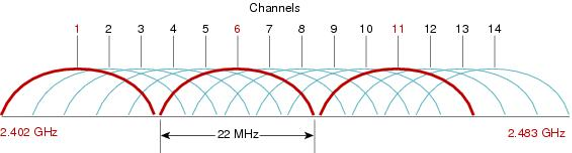
\includegraphics[width=\textwidth]{figs/2-4GHz}%
		\label{figs:2GHz-spectrum}}
	\\
	\subfloat[5GHz band]{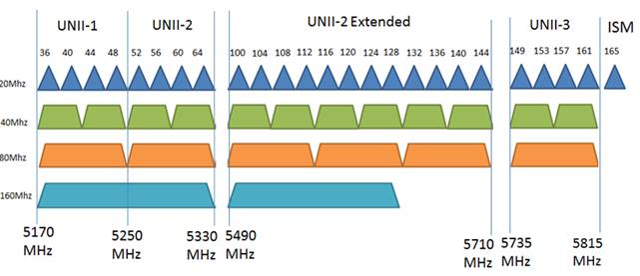
\includegraphics[width=\textwidth]{figs/5GHz}%
		\label{5GHz-spectrum}}
	\caption{$2.4$ GHz and $5$ GHz Unlicensed Spectrums.}
		\label{figs:2-5GHz-spectrum}
\end{figure}



\section{Frequency Channels}

The ETSI EN 301 893 V1.7.2 regulations \cite{LBT-ETSI-2014} released in July 2014 defined three unlicensed frequency bands as follows:
\begin{itemize}
\item
RLAN band 1: $5150$ to $5350$ MHz, divided into 2 sub-bands
\begin{itemize}
\item
Sub-band I: $5150$ MHz - $5250$ MHz. This sub-band is comparable to FCC U-NII-1. 
\item
Sub-band II: $5250$ MHz - $5350$ MHz. This sub-band is comparable to FCC U-NII-2.
\item
RLAN band 2: $5470$ MHz - $5725$ MHz. This band comparable to FCC U-NII-2 extended (U-NII-2e).
\item
RLAN band 3, also known as Broadband Radio Access Networks (BRAN): $5725$ – $5875$ MHz. This sub-band is comparable to FCC U-NII-3 ($5725$ – $5825$ MHz) band with a higher upper frequency range,.
\end{itemize}
\end{itemize}

Fig. \ref{5GHz-spectrum} summarizes radio channels defined in the $5$ GHz band by ETSI 301 893 standard (with a reference to FCC regulations). Technical details and the availability of each channel in four main regions (U.S., Europ, Japan, and China) are presented in Fig. \ref{figs:5GHz-spectrum-table}.

\begin{figure}[!t]
	\centering
	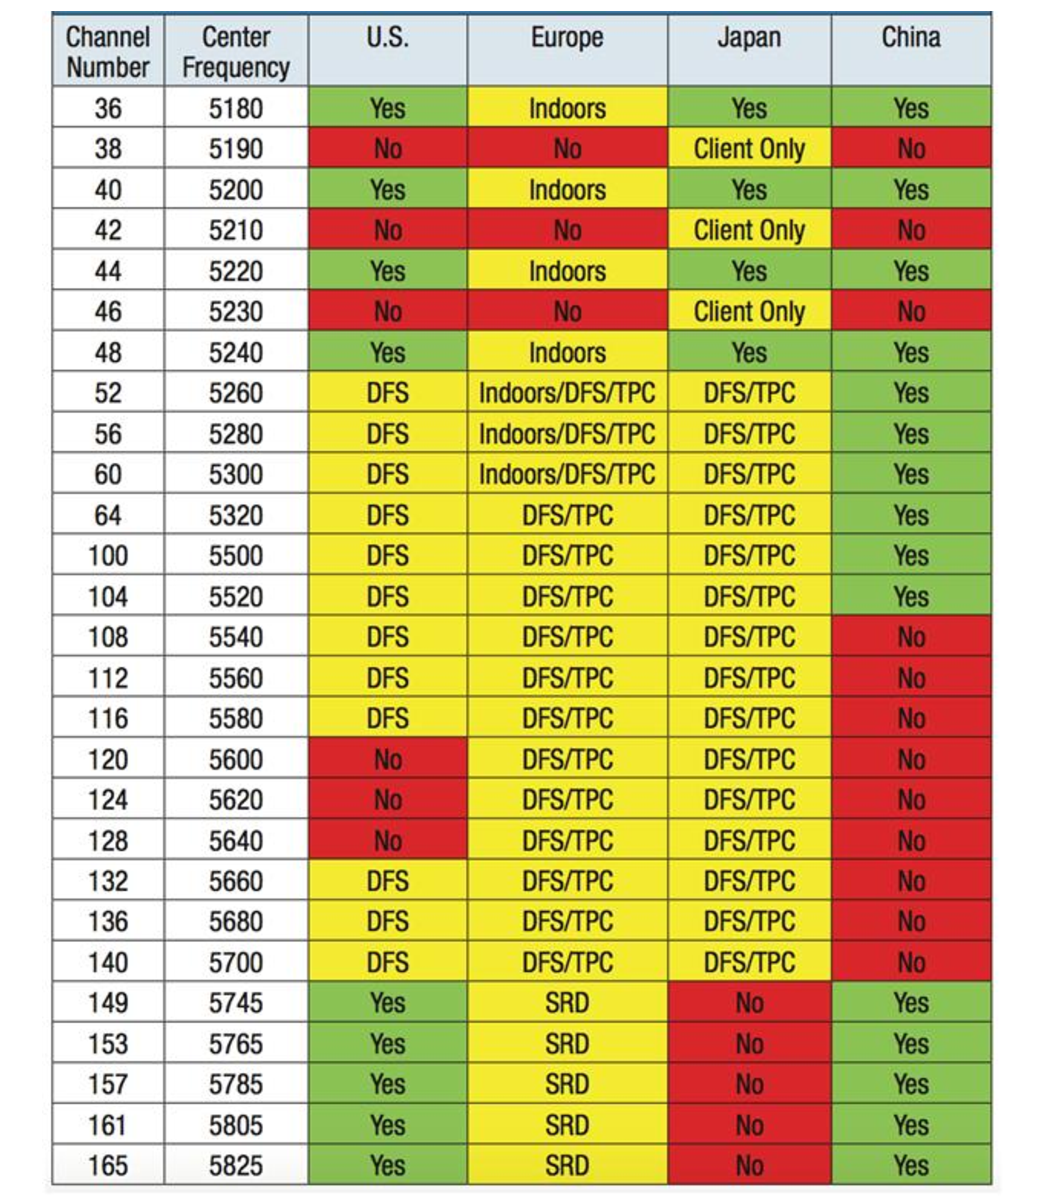
\includegraphics[width=0.85\columnwidth]{figs/5GHz-spectrum-table.pdf}
	\caption{Details of $5$ GHz Unlicensed Channels in Different Regions.}
	\label{figs:5GHz-spectrum-table}
\end{figure}


\section{Transmission Power}

Each of the three bands defined by ETSI EN 301 893 V1.7.2 regulations \cite{LBT-ETSI-2014} have different maximum allowable transmission power levels. Note that the RF output power is defined as the mean Equivalent Isotropic Radiated Power (EIRP) of the equipment during a transmission burst. In general, the limits are valid for the device with antenna gain and cable loss and not only the output power of WLAN module.

\subsection{RLAN band 1 ($5150$ to $5350$ MHz)}

\subsubsection{Indoor only Sub-band I ($5150$ - $5250$ MHz)}
The first RLAN sub-band includes the channels $36$ to $48$ and has an EIRP power limit to $23$ dBm ($200$ mW). These channels are considered for indoor only usage and do not require any Dynamic Frequency Selection (DFS) or Transmit Power Control (TPC) features. 

\subsubsection{Indoor only Sub-band II ($5250$ - $5350$ MHz)}
In the second sub-band of the RLAN band 1 with channels $52$ to $64$, the ETSI has set the EIRP power limit to $23$ dBm ($200$ mW) for devices with TPC and $20$ dBm ($100$ mW) for devices without TPC. For a device with TPC, the mean EIRP at the lowest power level of the TPC range must not exceed $17$ dBm ($50$ mW). This band requires DFS support and 

\subsection{RLAN band 2 ($5470$ to $5725$ MHz)}

Channels from $100$ to $140$ are part of the second RLAN band and have an EIRP power limit of $30$ dBm ($1000$ mW) for TPC and $27$ dBm ($500$ mW) for non-TPC devices or $20$ dBm ($100$ mW) for devices without any TPC or DFS support. The mean EIRP power level for a slave device with TPC must not exceed $24$ dBm at the the lowest TPC power level if the device is also capable of radar detection or $17$ dBm otherwise. 

\subsection{BRAN ($5725$ to $5875$ MHz)}

ETSI has defined the channels $155$ to $171$ (155, 159, 163, 167, 172) for Broadband Wireless Access (BWA) use only. The idea is to give internet access to locations without any wired access network available. The maximum EIRP output power has been set to $36$ dBm ($4000$ mW) with the limitation of RF power into antenna of $304$ dBm ($1000$ mW).


\section{Transmission Power Control (TPC)}

Dynamic adjustment of the transmission power is intended to reduce RFI. Dynamically adjusting the transmission power facilitates the shared use of the $5250$-$5350$ MHz and $5470$-$5725$ MHz frequency bands with satellite services. TPC determines the minimum transmission power necessary to maintain the connection with the partner (such as an access point).

If TPC is not used within these frequency bands, then the highest permissible average EIRP and the corresponding maximum EIRP density are reduced by $3$ dB. This restriction does not apply to the frequency range of $5150$-$5350$ MHz. Without DFS and TPC, a maximum of only $30$ mW EIRP is permitted. When DFS and TPC are used, a maximum $1000$ mW EIRP is permitted as the transmission power (compared with $100$ mW with 802.11 b/g, $2.4$ GHz, DFS and TPC are not possible here). The higher maximum transmission power not only compensates for the higher attenuation of $5$ GHz radio waves in air, it also makes noticeably longer ranges possible than in the $2.4$ GHz range. 


\section{Dynamic Frequency Selection (DFS)}

DFS was stipulated to (i) detect interference from radar systems (radar detection) and to avoid co-channel operation with these systems; and (ii) to provide on aggregate a near-uniform loading of the spectrum (Uniform Spreading). DFS is stipulated for the frequency ranges of $5250$-$5350$ MHz and $5470$-$5725$ MHz. It is optional for the frequency range of $5150$-$5250$ MHz.

DFS initially assumes that no channel is available in the corresponding frequency band. The WLAN device selects an arbitrary channel at the start and performs what is known as a Channel Availability Check (CAC). Before sending to a channel for $60$ seconds (Channel Observation Time, COT), a check is run to see if a different device is already working on this channel and the channel is therefore occupied. If this is the case, then a different channel is checked by the CAC. If not, then the WLAN device can perform the transmission operation. Even during operation, a check is run to see if a primary application such as a radar device is using this channel. This exploits the fact that radars frequently work according to the rotation method, whereby a tightly bundled directional transmission signal is transmitted by a rotating antenna. A remote receiver perceives the radar signal as a short pulse (radar peak). If a device receives such a radar peak, it pauses the transmission operation and monitors the channel for further pulses. If additional radar peaks occur during the COT, then a new channel is selected automatically. A check of this type is required to be carried out every $24$ hours. This is why interrupting the data transmission for $60$ seconds is unavoidable. 


\section{Channel Access Mechanisms}
\label{subsec:ETSI-overview}

In order to avoid channel collisions when two or more than two devices transmit the signal in the same channel at the same time, Listen Before Talk (BLT) strategy is employed. ETSI EN 301 893 V1.7.2 \cite{LBT-ETSI-2014} describes two mechanisms that require an equipment or a device to apply CCA before using the channel. The first mechanism is Frame Based Equipment (FBE) which defines a fixed (not directly demand-driven) timing frame for channel access. The second mechanism is Load Based Equipment (LBE) which defines demand-driven timing frame.

\begin{figure}[!t]
	\centering
	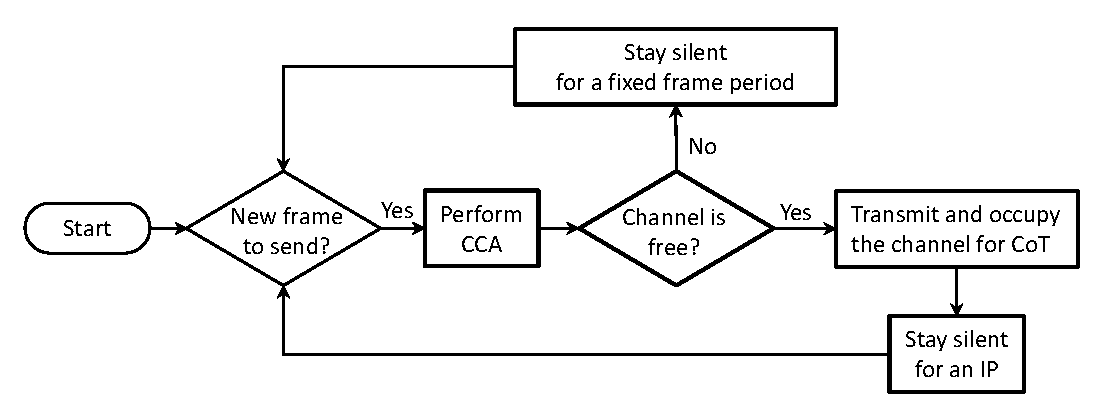
\includegraphics[width=0.9\columnwidth]{figs/FBE-flowchart}
	\caption{Simplified flowchart of FBE.}
	\label{figs:FBE-flowchart}
\end{figure}

\begin{figure}[!t]
	\centering
	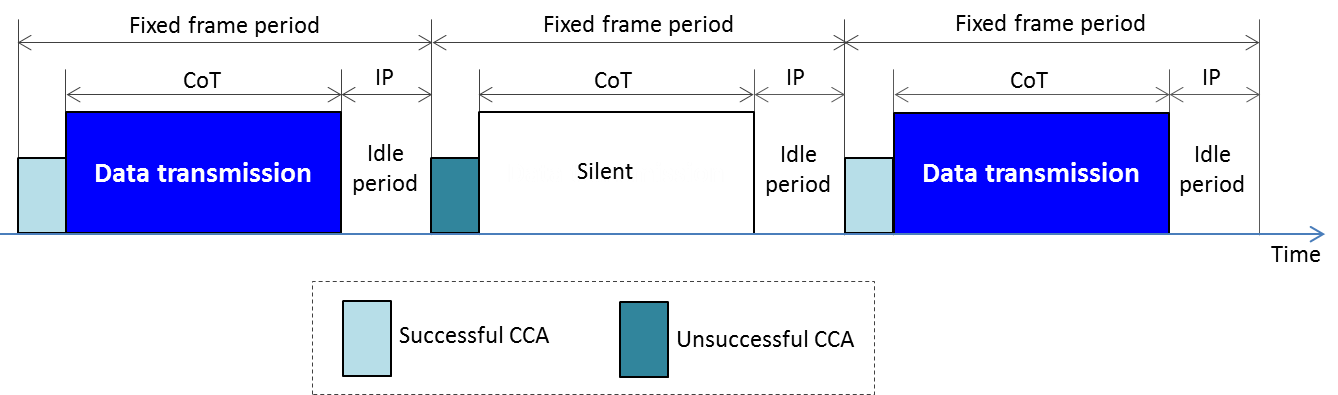
\includegraphics[width=0.9\columnwidth]{figs/FBE-example}
	\caption{An illustrative example of FBE.}
	\label{figs:FBE-example}
\end{figure}


\subsection{FBE-based Mechanism}
\label{etsi-lbt:fbe}

FBE shall comply with the following requirements:

\begin{itemize}
	
	\item
	\textit{R1:} Before starting transmissions on an operating channel, the equipment shall perform a CCA check using Energy Detect (ED). The equipment shall observe the channel for the duration of the \textit{CCA observation time}. The operating channel shall be considered occupied if the energy level in the channel exceeds the \textit{threshold} corresponding to the power level.
	
	\item
	\textit{R2:}
	If the CCA procedure finds the channel clear, the equipment may transmit immediately and occupy the channel for a \textit{fixed time period}.
	
	\item
	\textit{R3:} If the CCA procedure finds the channel occupied, the equipment shall not transmit on that channel during the next fixed frame period.
	
	\item
	\textit{R4:} The total time during which an equipment has transmissions on a given channel without re-evaluating the availability of that channel is defined as the \textit{Channel Occupancy Time} (CoT).
	
	\item
	\textit{R5:} After occupying the channel for CoT, the equipment keeps silent and waits for a short time, namely \textit{Idle Period} (IP).
	
	\item
	\textit{R6:} Towards the end of the idle period, the equipment shall perform a new CCA procedure as described in R1 above.
	
	\item
	\textit{R7:} The equipment, upon correct reception of a packet which was intended for this equipment, can skip CCA and immediately proceed with the transmission of management and control frames, e.g., acknowledgment (ACK) and block ACK frames.
	
	\item
	\textit{R8:}
	A consecutive sequence of such transmissions by the equipment, without it performing a new CCA, shall not exceed the maximum CoT.
	
	\item
	\textit{R9:}
	CCA observation time shall be not less than $20$ $\mu$s.
	
	\item
	\textit{R10:} CoT shall be in the range from $1$ ms to $10$ ms.
	
	\item
	\textit{R11:}
	The minimum IP shall be at least $5$\% of CoT used by the equipment for the current fixed frame period.
	
\end{itemize}

A simplified flowchart and an illustrative of FBE are given in Figs. \ref{figs:FBE-flowchart} and \ref{figs:FBE-example}, respectively.


\begin{figure}[!t]
	\centering
	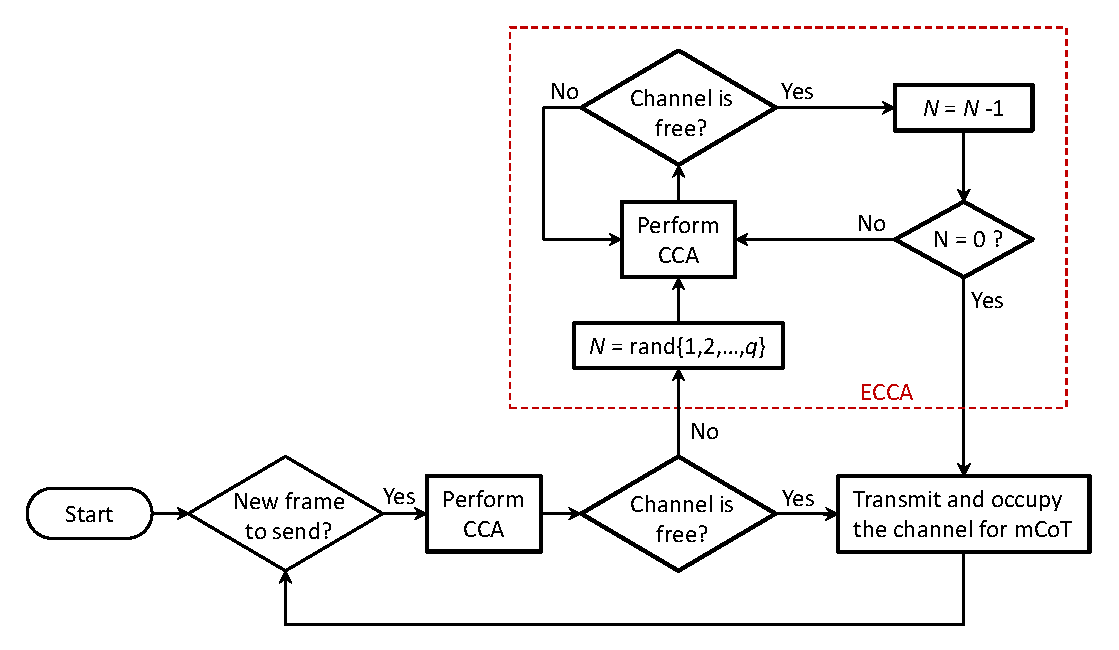
\includegraphics[width=0.9\columnwidth]{figs/LBE-flowchart}
	\caption{Simplified flowchart of LBE.}
	\label{figs:LBE-flowchart}
\end{figure}

\begin{figure}[!t]
	\centering
	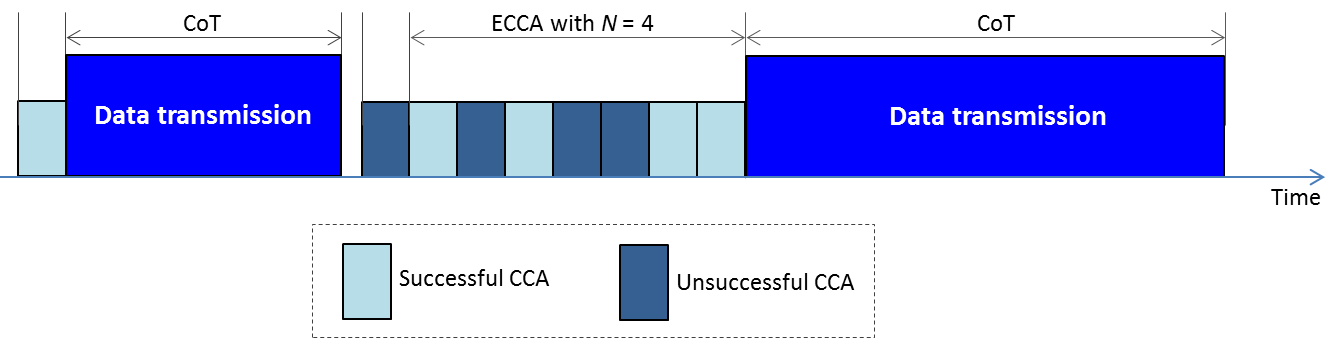
\includegraphics[width=0.9\columnwidth]{figs/LBE-example}
	\caption{An illustrative example of LBE.}
	\label{figs:LBE-example}
\end{figure}


\subsection{LBE-based Mechanism}
\label{etsi-lbt:lbe}

LBE shall comply with the following requirements:

\begin{itemize}
	
	\item
	\textit{R1:} Before starting transmissions on an operating channel, the equipment shall perform a CCA check using ED. The equipment shall observe the channel for the duration of the \textit{CCA observation time}. The operating channel shall be considered occupied if the energy level in the channel exceeds the threshold corresponding to the power level.
	
	\item
	\textit{R2:}
	If the CCA procedure finds the channel clear, the equipment may transmit immediately on that channel.
	
	\item
	\textit{R3:}
	If the CCA procedure finds the channel occupied, it shall not transmit in that channel. The equipment shall perform an Extended CCA (ECCA) procedure in which the channel is observed for a random duration.
	
	\item
	\textit{R4:}
	If the ECCA procedure has determined the channel to be clear, the equipment may start transmissions on this channel.
	
	\item
	\textit{R5:}
	The total time that an equipment makes use of the channel (without performing CCA) is the \textit{maximum Channel Occupancy Time} (mCoT), after which the device shall perform a new CCA procedure as described in R1 above.
	
	\item
	\textit{R6:}
	The equipment, upon correct reception of a packet which was intended for this equipment, can skip CCA and immediately proceed with the transmission of management and control frames, e.g., ACK and block ACK frames.
	
	\item
	\textit{R7:}
	A consecutive sequence of transmissions by the equipment, without it performing a new CCA, shall not exceed mCoT.
	
	\item
	\textit{R8:}
	CCA observation time shall be not less than $20$ $\mu$s.
	
	\item
	\textit{R9:}
	The random duration in an ECCA procedure is $N \times$ (CCA observation time), where $N$ is randomly selected in the range $\{1,2,...,q\}$, $q \in \{4,5,...,32\}$ (declared by the manufacturer).
	
	\item
	\textit{R10:}
	mCoT should be less than $(13/32)\times q$ ms (mCoT is in the range from $1.625$ to $13$ ms).
	
\end{itemize}

A simplified flowchart and an illustrative of LBE are given in Figs. \ref{figs:LBE-flowchart} and \ref{figs:LBE-example}, respectively.


%%%%%%%%%%%%%%%%%%%%%%%% referenc.tex %%%%%%%%%%%%%%%%%%%%%%%%%%%%%%
% sample references
% %
% Use this file as a template for your own input.
%
%%%%%%%%%%%%%%%%%%%%%%%% Springer-Verlag %%%%%%%%%%%%%%%%%%%%%%%%%%

\begin{thebibliography}{99.}%
\bibitem{LBT-ETSI-2014}
\emph{ETSI EN 301 893 V1.7.2 (2014-07): Broadband Radio Access Networks (BRAN); 5 GHz high performance RLAN; Harmonized EN covering the essential requirements of article 3.2 of the R\&TTE Directive}, European Telecommunications Standards Institute Std., 2014.
\end{thebibliography}

%%%%%%%%%%%%%%%%%%%%% chapter.tex %%%%%%%%%%%%%%%%%%%%%%%%%%%%%%%%%
%
% sample chapter
%
% Use this file as a template for your own input.
%
%%%%%%%%%%%%%%%%%%%%%%%% Springer-Verlag %%%%%%%%%%%%%%%%%%%%%%%%%%

%\motto{Use the template \emph{chapter.tex} to style the various elements of your chapter content.}
\chapter{LTE-Advanced: An Overview}
\label{overview-lte} % Always give a unique label
% use \chaptermark{}
% to alter or adjust the chapter heading in the running head

\abstract*{This chapter provides a high-level overview of LTE-Advanced (LTE-A) networks and associated technologies to form a basis for discussion of the co-existence issues that exist for unlicensed LTE and Wi-Fi. Understanding the underlying architecture and protocols employed in LTE-A networks will provide readers a comparative framework to grasp how, and at what levels, LTE and Wi-Fi networks may interact and interfere with each other, and form a greater understanding of the challenges to be address in designing coexistence mechanisms. Specifically, this chapter will overview the LTE-A network, its capabilities and protocols, with specific emphasis on the physical layer and medium access sub-layers to illuminate specific sources of co-existence issues. Proposed changes which may be included in future LTE releases are discussed in the context of LTE/Wi-Fi coexistence.}

This chapter provides a high-level overview of LTE-Advanced (LTE-A) networks and associated technologies to form a basis for discussion of the co-existence issues that exist for unlicensed LTE and Wi-Fi. Understanding the underlying architecture and protocols employed in LTE-A networks will provide readers a comparative framework to grasp how, and at what levels, LTE and Wi-Fi networks may interact and interfere with each other, and form a greater understanding of the challenges to be address in designing coexistence mechanisms. Specifically, this chapter will overview the LTE-A network, its capabilities and protocols, with specific emphasis on the physical layer and medium access sub-layers to illuminate specific sources of co-existence issues. Proposed changes which may be included in future LTE releases are discussed in the context of LTE/Wi-Fi coexistence.


\section{System Overview}
\label{sys-overview}
The enhancements to the Long Term Evolution/System Architecture Evolution (LTE/SAE) to meet the requirements set out for fourth generation (4G) cellular networks are collectively known as LTE-Advanced (LTE-A).  The LTE-A requirements were formalized by the 3rd Generation Partnership Project (3GPP) in LTE releases 10 through 13 \cite{tr36913}.  LTE itself was a logical evolution from the technologies used in previous generations in order to meet the increasing demands for higher data rates and improved quality of service. LTE met these demands at the access level through increased spectral efficiency and improved mobility support and cell edge data rates.  The increased spectral efficiency was achieved by using orthogonal frequency division multiple access (OFDMA) and single-carrier frequency division multiple access (SC-FDMA) in the downlink and uplink, respectively.  Improvements in mobility support and cell edge data rates were achieved through enhanced adaptive modulation and bandwidth selection and downlink spatial multiplexing and multiple input/multiple output support.  Beyond the access layer, LTE transitioned to an all IP packet switched core network with the introduction of the evolved packet core, and a flattened network architecture of enhanced base stations called evolved NodeB's (eNB) interconnected via high-speed data links.  Combined, these fundamental changes to the cellular network architecture have allowed LTE networks to significantly increase user data rates and reduce control and user plane latency and connection set-up and handover times.  LTE-A represents the further, and ongoing, evolution of cellular networks to continue to meet the every increasing demands for higher data rates, user mobility support, and efficient support of a growing number of wireless devices.

\subsection{Network Architecture}
\label{net-arch}
The requirements to provide high data rates while supporting high-speed mobility requires the ability to set up and tear down user connections and manage inter-cell handoffs with as little latency as possible.  In previous generations of cellular networks, a hierarchical structure consisting of base stations or NodeBs connected to a central controller had been used.  This star or cluster architecture requires additional hops in both data transmissions and hand off negotiation which can introduce significant delay.  Controllers were are responsible for managing all data and control traffic, as well as handoffs betweens several pairs of base stations.  For many increasingly ubiquitous end-user applications, such as online gaming and voice/video over the internet, the additional latency in connection set up and handover can impair the user-perceived quality of experience.
\begin{figure}[!ht]
	\centering
	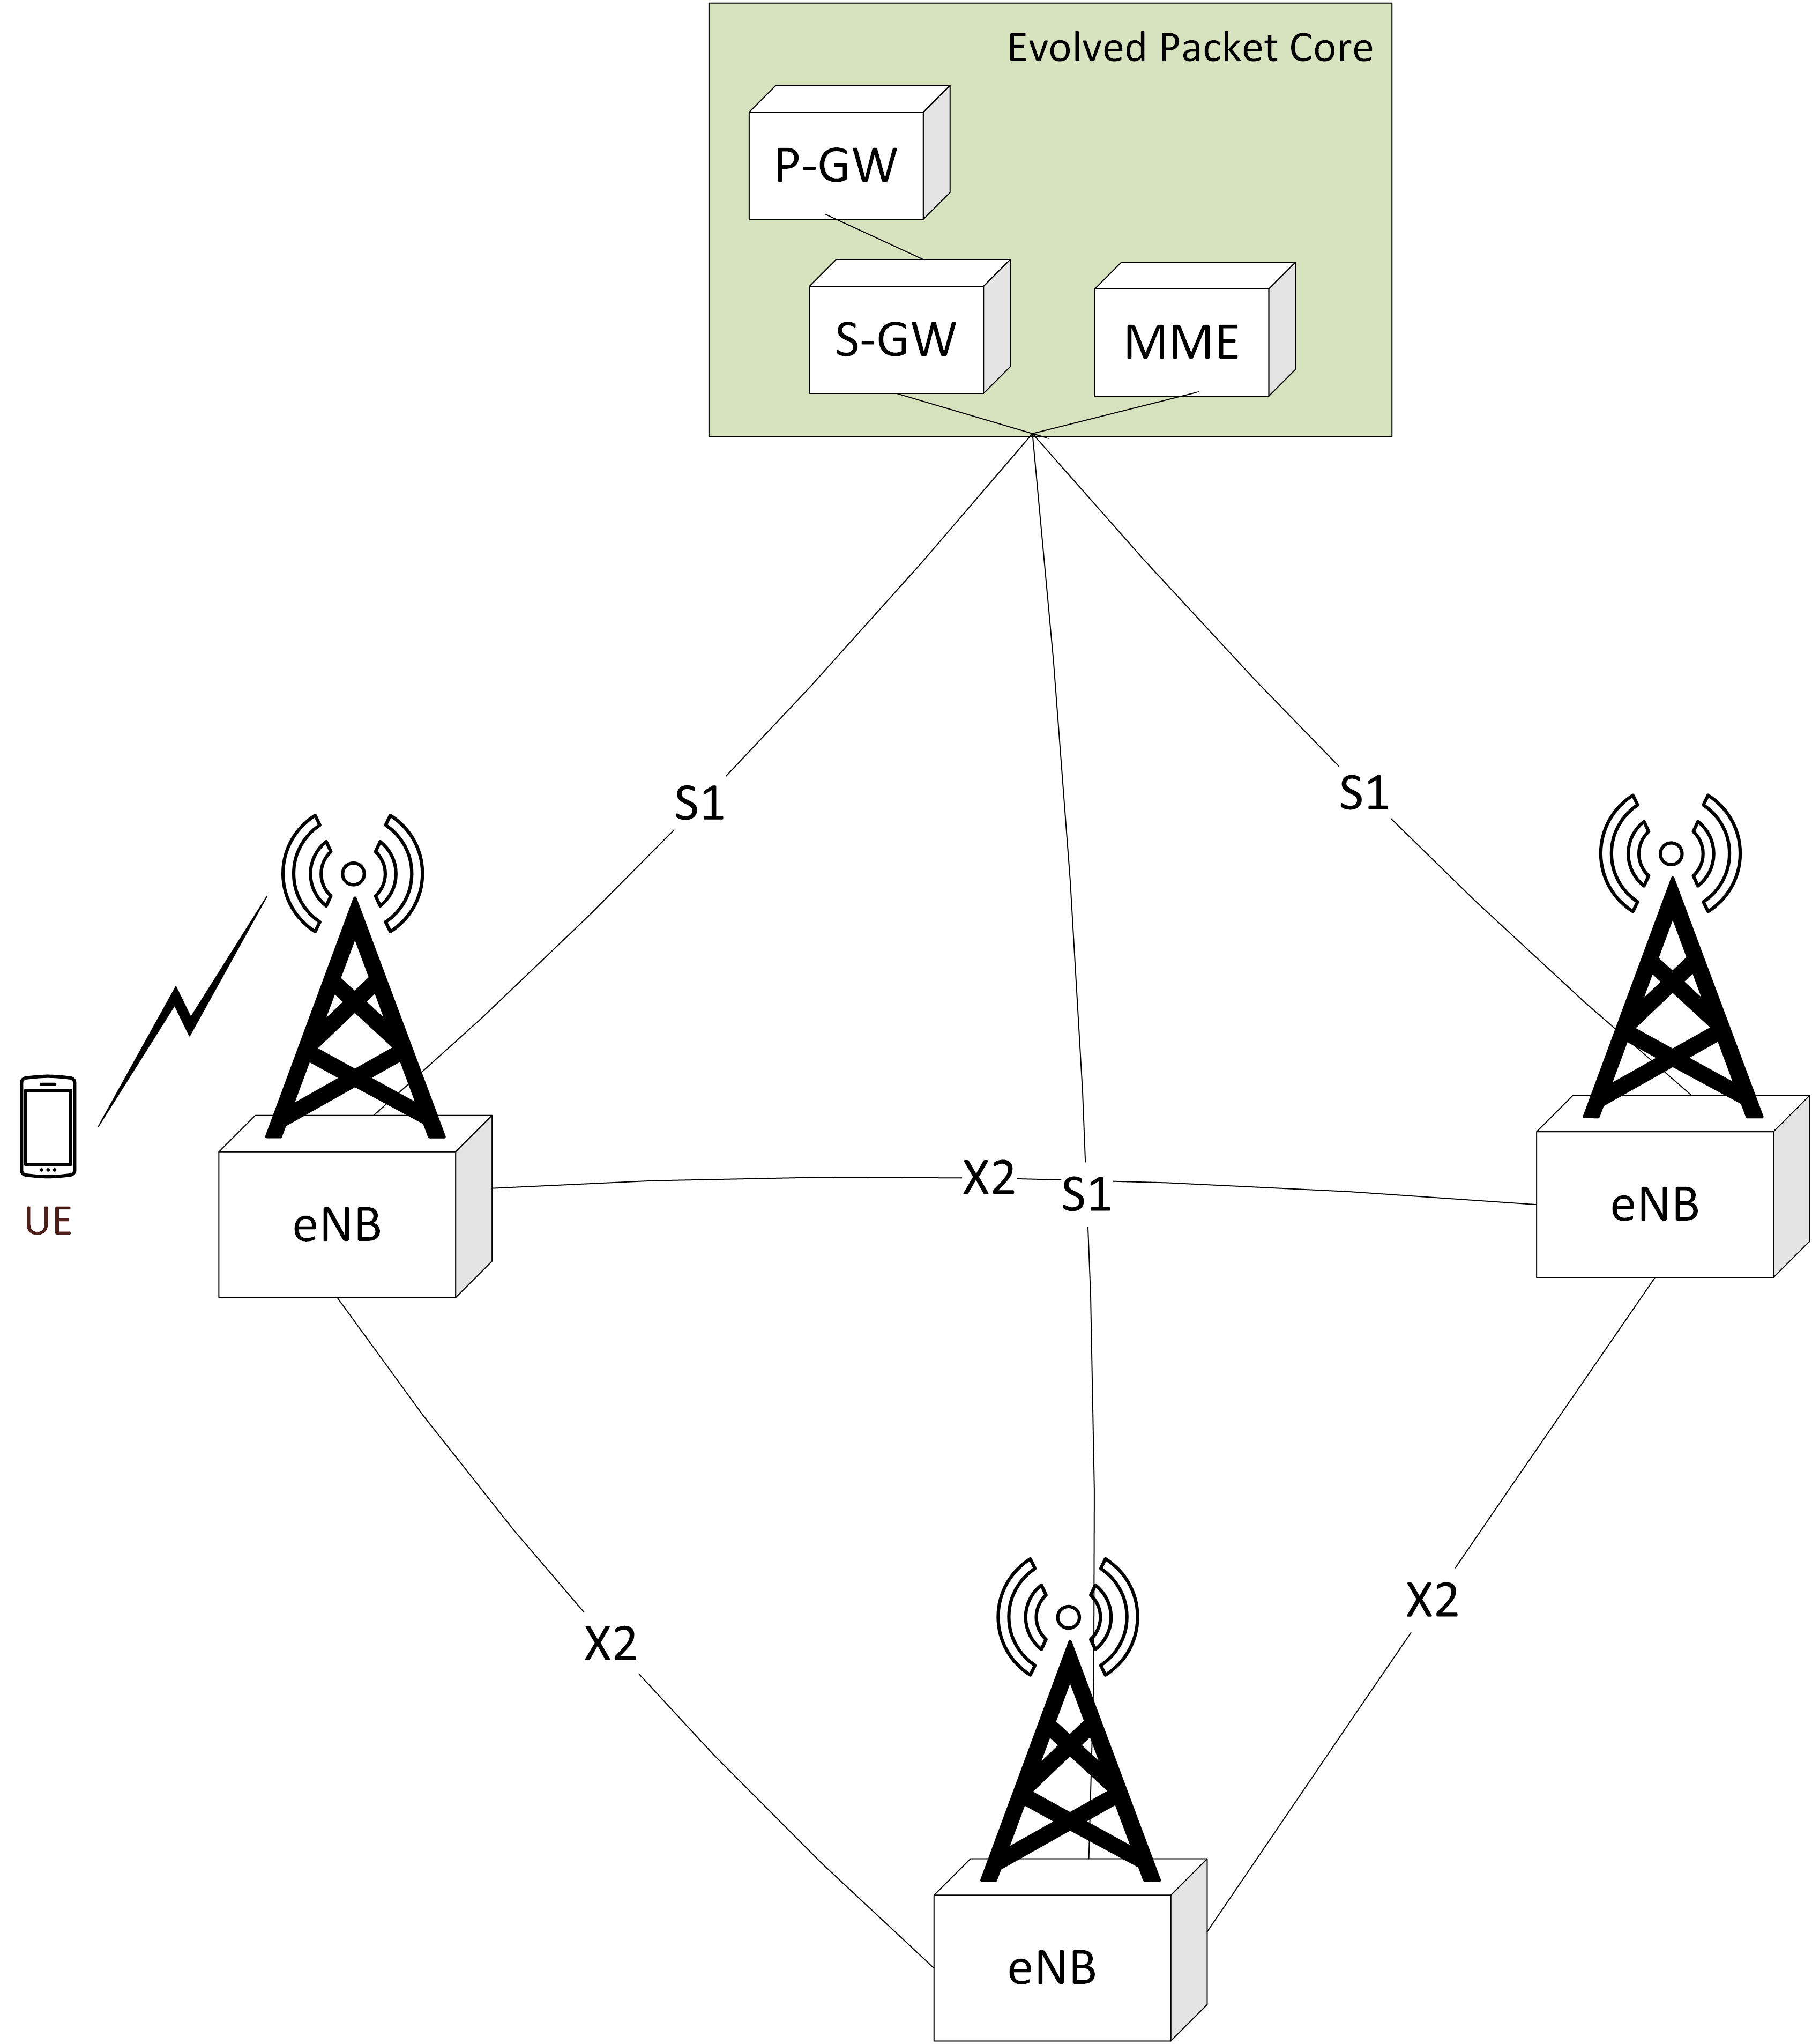
\includegraphics[width=0.58\textwidth]{figures3/lteAnet}
	\caption{Basic structure of LTE cellular networks.}
	\label{figs:LTE-A-Network}
\end{figure}

The flat architecture adopted by LTE networks is depicted in Fig. \ref{figs:LTE-A-Network}.  The migration of local functions to eNBs and global functions to the EPC were driven by the requirements of reduced latency and higher data rates. The functions of radio network and medium access control, handoff requests, negotiations, and management, as well as some other truly local functions, are migrated to the eNBs, which are interconnected via high-speed, low latency, connections in a mesh configuration \cite{tr36300}.  The low-latency X2 interface connections between eNBs allows for fast user handover, including forwarding of queued data for seamless user experience.  Additionally, with direct connections between neighboring cells, this architecture facilitates more effective multi-point transmission and coordination and inter-cell interference and load management, independent of conditions in other areas of the network. The global functions and connections to external networks are handled at the evolved packet core (EPC). The functional split between the various components of the network, as well as the implementation of the necessary layers of the network protocol stack, is shown in further detail in Fig. \ref{figs:funcSplit}.
\begin{figure}[!Ht]
	\centering
	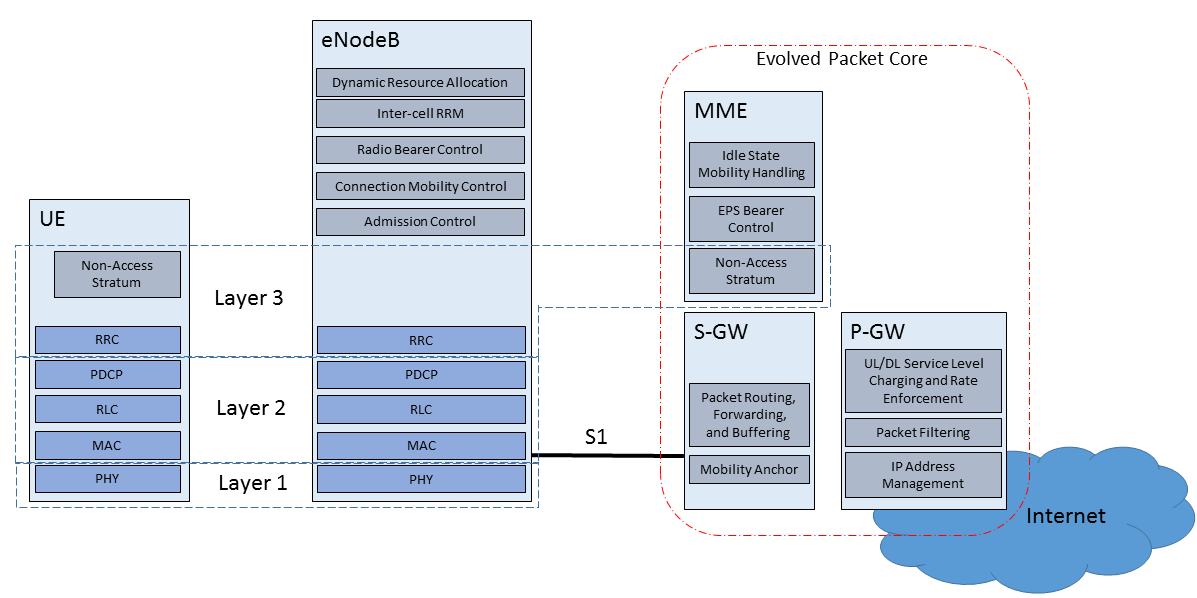
\includegraphics[width=\textwidth]{figures3/LTE-decomp}
	\caption{Functional split between various entities in LTE under the system architecture evolution.}
	\label{figs:funcSplit}
\end{figure}
In addition to those listed in the figure, the mobile management entity (MME) handles authentication, authorization and accounting functions.  The packet data network gateway (P-GW) and serving gateway (S-GW) handle user data packet forwarding, filtering, and usage tracking, as well as acting as a mobility anchor for inter-eNB and inter-RAT handovers.  Further, the distributed radio network and resource management and medium access control allows eNBs to quickly adapt to changing radio medium condition and provide timely user scheduling based on local information.

\subsection{Capabilities and Features}

While the gains made by LTE were significant, they fell short of the requirements set out for 4G networks by the International Telecommunications Union, specifically in the case of peak data rates, spectral efficiency, and cell edge performance \cite{itu-advanced}.  The continuing evolution which became LTE-A was finally able to achieve the necessary targets to meet the ITU requirements for 4G.  Some important ITU requirements, and achieved performance levels for LTE and LTE-A, are highlighted in Table \ref{perf-table}.

\begin{table}
	\caption{ITU-A Requirements for 4G vs. LTE/LTE-A Achievements \cite{lte-3gpp}\cite{lteA-3gpp}\cite{itu-advanced}\cite{abdullah}}
	\label{perf-table}      
	\begin{tabular}{p{0.5\textwidth}p{0.15\textwidth}p{0.15\textwidth}p{0.15\textwidth}}
		\hline\noalign{\smallskip}
		Description/Requirements & ITU-A & LTE & LTE-A   \\
		\noalign{\smallskip}\svhline\noalign{\smallskip}
		DL peak spectral efficiency (bps/Hz) &  15   & 15  & 30 \\
		UL peak spectral efficiency (bps/Hz)& 6.75  & 3.75  & 15 \\
		Min. cell edge spectral \\ \hspace{0.8em} efficiency (bps/Hz) & 0.04 & 0.024 & 0.04 \\
		DL Peak data rates (Mbps) & 1000$^1$  & 300 & 1000 \\
		UL Peak data rates (Mbps) & 1000$^1$  & 75 & 500 \\
		Scalable bandwidth up to (MHz) & 40 & 20  & 100$^2$ \\
		
		\noalign{\smallskip}\hline\noalign{\smallskip}
	\end{tabular}
	$^1$ For low mobility with requirement of min. 100 Mbps for speeds of up to 350 km/h. 	 \\
	$^2$ With carrier aggregation of up to five carrier components.
\end{table}

Among other innovations, in order to meet these requirements, LTE-A extended bandwidth scalability in LTE by supporting carrier aggregation, both within and across frequency bands.   Discontiguous aggregation is supported to ensure a higher bandwidth is available for providers who cannot support it in contiguous spectrum allotments, allowing the development of license-assisted access (LAA-LTE) into the unlicensed and TV whitespace bands.  Backwards compatibility is maintained by using bandwidths for each carrier component which match those used in LTE.  LTE-A also expands MIMO/spatial multiplexing support up to 8x8 for DL and 4x4 for UL, adds coordinated multi-point operation to increase spectral efficiency and cell edge data rates, and improves heterogeneous network planning with the enhancement of support for small cells and relay nodes to increase area coverage with reduced power requirements.

\section{Channel Access Mechanisms}
\label{channel-access}
Like other cellular access technologies, LTE-A has been designed for use on dedicated licensed spectrum allocations where there is, generally, no need to contend for channel access.  While interference, fading, and path loss can corrupt LTE transmissions, and recovery and retransmission functions are necessary, in general a centrally controlled and tightly scheduled channel access mechanism is able to guarantee service levels required by all uplink (UL) and downlink (DL) traffic \cite{tr36300}. UL/DL seperation is achieved through either time-division duplexing (TDD) or frequency-division duplexing (FDD).  Orthogonal frequency-division multiple access (OFDMA) is used in the DL, allowing the eNB to efficiently schedule transmissions for many users in the same transmission time interval.  Single-carrier frequency-division multiple access (SC-FDMA) is used in the uplink in order to reduce the power consumption requirements of battery-dependent user equipment (UE) to communicate with the eNB.  Further, coordinated multipoint (CoMP) is supported by allowing UEs to be configured to process channel state information from multiple eNBs, and both single-user (SU) and multi-user (MU) MIMO are supported in multiple configurations to achieve transmit diversity or multi-layer transmissions with beamforming possible in both horizontal and vertical dimensions.

The basic structure of the protocol stack used in LTE networks to facilitate channel access is shown in Fig. \ref{figs:stack} \cite{tr36201}.
\begin{figure}[!ht]	
	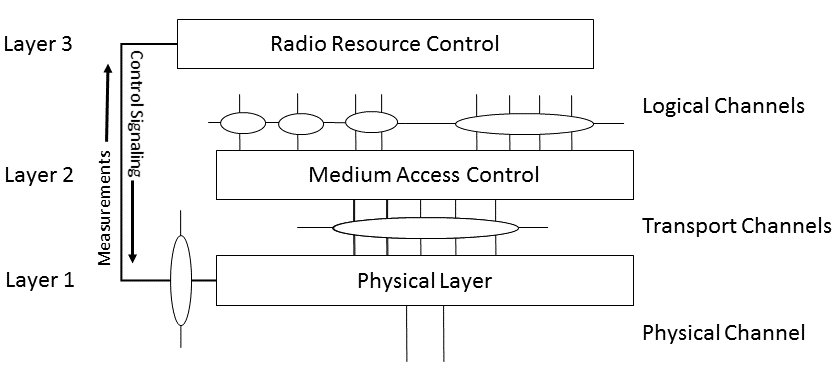
\includegraphics[width=\textwidth]{figures3/LTEradio-interface}
	\caption{E-UTRA radio interface protocol architecture.}
	\label{figs:stack}
\end{figure}
UL and DL transmissions are divided amongst several physical channels, according to the type of transmission, i.e. user traffic or control information, and the type of transmission, i.e broadcast or unicast and scheduled or random access (random access is primarily used by a UE which has not yet associated to an eNB). The information bearing physical channels are mapped by the PHY layer into transport channels supplied to the MAC sublayer, which in turn remaps these into several logical channels provided to the higher layers. 

\subsection{LTE-A Physical Layer}
\label{lte-phy}
The LTE PHY layer is designed to be both highly adaptable as well spectrally and power efficient.  In the DL, OFDMA is used to schedule many signals in the same transmission time interval and achieve a high spectral efficiency, however, the very high peak to average power ratio makes this multiple access strategy unattractive in the UL for battery-dependent devices \cite{tr36201}\cite{tr36211}.  SC-FDMA is used in the UL to maintain a satisfactory spectral efficiency while significantly improving power efficiency and battery life. Example carrier allocations for both DL and UL are shown in Fig. \ref{lte:of-sc-fdma}.
\begin{figure}[!ht] 	
	\subfloat[OFDMA used in downlink.]{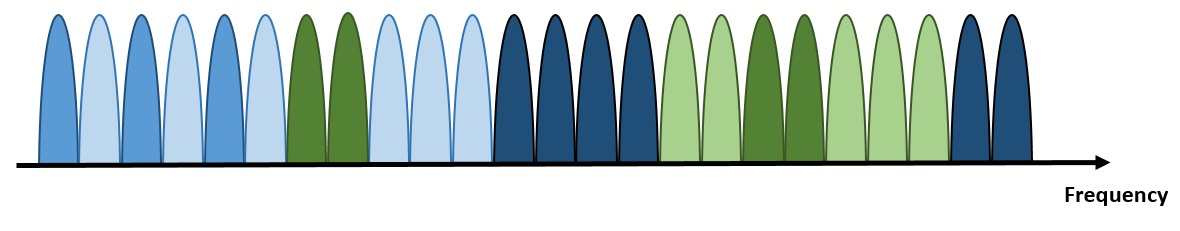
\includegraphics[width=\textwidth]{figures3/ofdma}%
		\label{ofdma}}
	\\
	\subfloat[SC-FDMA used in uplink.]{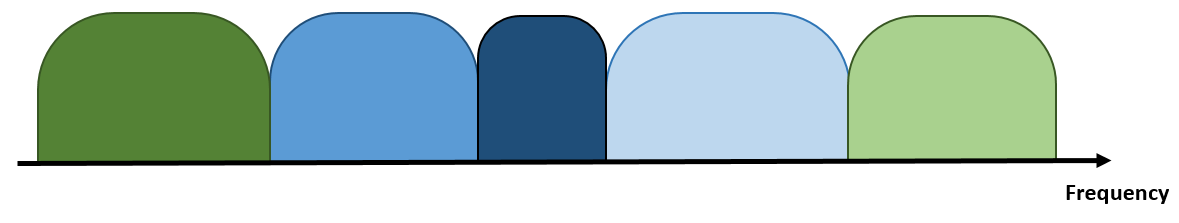
\includegraphics[width=\textwidth]{figures3/sc-fdma}%
		\label{sc-fdma}}
	\caption{Multiple access strategies used in LTE for uplink and downlink.}
	\label{lte:of-sc-fdma}
\end{figure}
Each color and shade represents the carriers allocated to a specific user.  The assignment of sub-carriers to a given UE are driven by the specific loss and interference experienced by that user, called channel state information (CSI), in order to maximize the overall achieved rate of all users.  As shown in Fig. \ref{ofdma}, in the DL LTE-A supports both localized (contiguous) and distributed allocations, to best use CSI to maximize network efficiency. Sub-carrier assignments can further span disjoint frequency bands, including into unlicensed bands.  In Fig. \ref{sc-fdma}, which depicts an example UL allocation, a given sub-carrier, with variable bandwidth, is assigned to a single UE, again based on CSI.  It should be emphasized that Fig. \ref{lte:of-sc-fdma} shows a single instant of time, over subset of the available band. 

All transmission are organized into frames comprised of twenty slots, every two of which comprise a subframe \cite{tr36211}. An example of one configuration for the LTE frame structure is shown in Fig. \ref{lte:frame}.
\begin{figure}[!t]
	\centering
	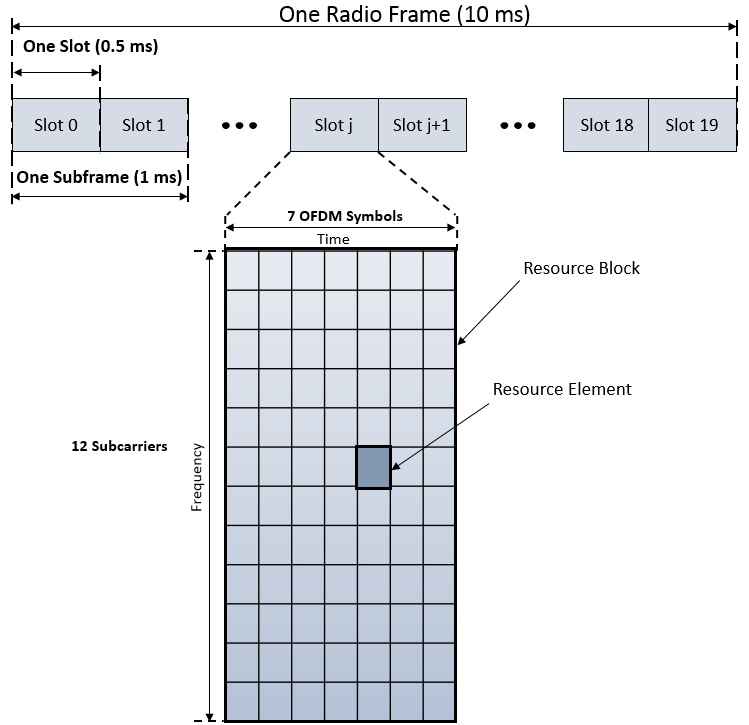
\includegraphics[width=0.8\textwidth]{figures3/LTE-frame}
	\caption{LTE frame and resource block structure.}
	\label{lte:frame}
\end{figure}
A single sub-carrier, with either 7.5 or 15 kHz bandwidth, paired with a transmission duration required to transmit a single OFDM symbol is called a resource element.  The minimum unit which can be allocated to a physical channel or user is the physical resource block (PRB).  For simplicity, in the breakout, a single PRB is depicted, though a single PRB spans only a small subset of the available sub-carriers. Depending on the configuration used, a PRB is formed of either 7, 6, or 3 OFDM symbols and 12 or 24 sub-carriers allocated for one 0.5 ms slot.  Between 6 and 10 PRBs will then be allocated to UE in order to achieve bandwidths between 1.4 and 20 MHz (though the occupied bandwidth will be smaller, 1.08 to 18 MHz).  Higher bandwidths are achieved through carrier aggregation in the same slot, either contiguous or not. 

Two distinct frame structures are defined to support both time division duplexing (TDD) and frequency division duplexing (FDD), as well as a third frame structure specifically for license assisted access (LAA-LTE).  All three frame types have the same basic structure shown in Fig. \ref{lte:frame}, with the differences being in how transmission are scheduled.  Both half and full duplex are supported in FDD and all 10 subframes are available for both UL and DL.  In half duplex configurations, transmission are seperated in both time and frequency, while for full duplex transmissions separation is in frequency only.  For TDD, the frame is organized into two 5 ms half-frames, with several UL/DL configurations and switching patterns supported.  As of Release 13, the special frame structure defined for LAA-LTE reserves all 10 subframes for DL, with transmission able to occupy one or more consecutive subframes, but required to start somewhere within the first subframe. LAA-LTE is expected to be expanded to support both UL and DL in future releases.

Beyond the features discussed in detail, the LTE-A PHY layer provides forward error correction and automatic repeat request functions, modulation/demodulation of physical signals, mapping and rate matching of physical channels to transport channels, frequency and time synchronization, and MIMO antenna processing, including transmit diversity and beamforming.  A variety of modulation schemes are supported depending on channel conditions, distance from receiver, and power requirements (up to 256 QAM in the downlink).  

\subsection{LTE-A Medium Access Control}
\label{lte-mac}
Medium access in LTE is tightly controlled and scheduled in both UL and DL, with the eNB controlling the time and frequency resource block assignment for all but random access channels (used for UE connection requests and some other procedures) \cite{tr36321}.  Distinct MAC sublayers for the eNB and the UE are defined, optimized to their specific functions and resources.  Additionally, several MAC configurations are defined for UE depending on the specific functions implemented, such as dual connectivity to support Coordinated Multipoint (CoMP) transmission and sidelink channels for UE device-to-device communication. The basic structure of the MAC sublayer, without CoMP or sidelink configured, is shown in Fig. \ref{figs:lte-mac}.
\begin{figure}[!ht]
	\centering
	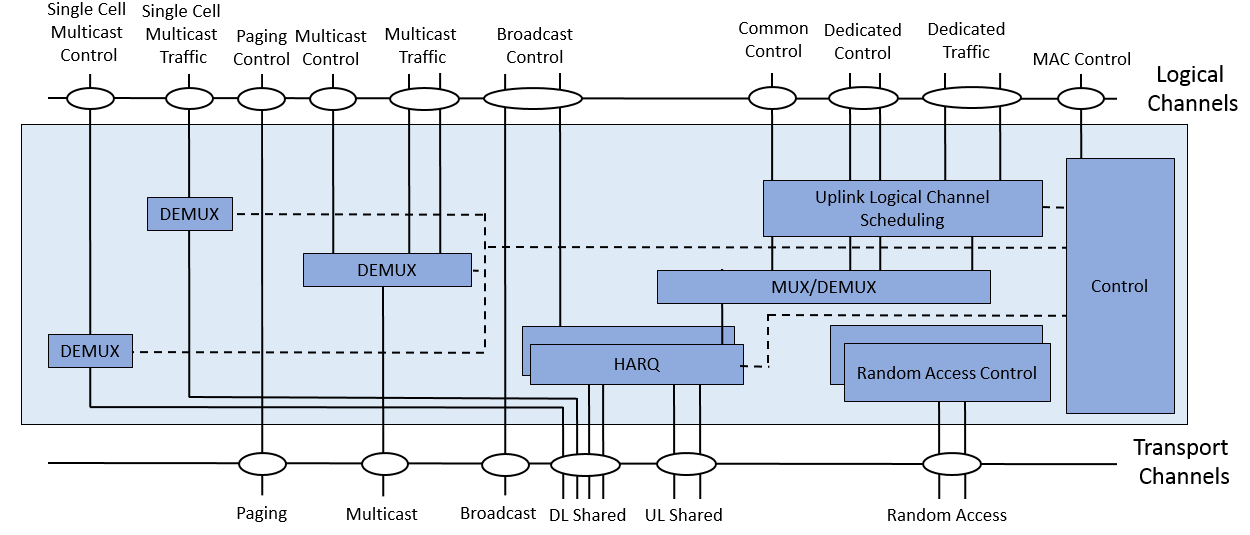
\includegraphics[width=\textwidth]{figures3/LTE-MAC}	
	\caption{LTE MAC sublayer structure and channel mapping.}
	\label{figs:lte-mac}
\end{figure}
The extension to other MAC configurations requires the duplication of this basic structure, and separate control and traffic channels required. In dual connectivity, for example, two such MAC structures are implemented for the master and secondary cell group, however only the broadcast, shared UL and DL, and random access channels are needed for the secondary cell group.  In sidelink configuration, only broadcast, discovery and duplex UL/DL shared channels are required.

The MAC sublayer facilitates reliable data transfer through radio resource allocation, UL traffic prioritization in the UE, and the mapping and multiplexing between transport channels and one or more logical channels. Further, the MAC sublayer handles hybrid automatic repeat requests (HARQ) signaling, a combination of forward error correcting coding and error detection, as well as channel prioritization with dynamic scheduling, random access control, and scheduling information reporting and requests.

The specific implementation of these, and other layer 2 functions such as radio link control, are quite complex and beyond the scope of this brief, however the underlying design paradigm is that of global knowledge facilitating tight control over medium access. The MAC sublayer in the eNB is aware of the channel conditions for each UE to be scheduled in both the UL and DL, and the UE adheres to the schedule of time and frequency provided by the eNB.  PRBs are assigned to UL and DL transmissions to achieve the greatest advantage from local channel conditions. Little consideration of inter-user or inter-carrier interference is necessary, due to the dedicated frequency bands and orthogonal carriers discussed in Sec. \ref{lte-phy}.  As a result, LTE-A is able to achieve high spectral efficiency and reliability.


\section {Changes Expected for Future Releases}
\label{fut-chnge}
LTE-A brings cellular networks into the realm of 4G, as defined by \cite{itu-advanced}.  As far as LTE-A has taken us, it will not be enough for fifth generation (5G) networks which are expected to support existing and new use cases ranging from smart cities and Internet of Things devices (massive machine type communication) to self-driving vehicles and industrial automation (ultra-reliable and low latency communications) with  high speed mobile broadband on the order of giga\emph{bytes} per second \cite{itu-2020}.  Some of the specific requirements are outlined in Table \ref{5g-table}.
\begin{table}
	\caption{ITU-A Requirements for 4G vs. ITU-2020 Requirements for 5G  \cite{itu-2020}}
	\label{5g-table}      
	\begin{tabular}{p{0.6\textwidth}p{0.18\textwidth}p{0.18\textwidth}}
		\hline\noalign{\smallskip}
		Description/Requirements & ITU-A & ITU-2020  \\
		\noalign{\smallskip}\svhline\noalign{\smallskip}
		Peak data rates (Gbps) & 1  & 20\\
		Average user data rates (Mbps) & 1  & 100  \\				
		Mobility support(km/h) & 350  & 500 \\
		Connection density (devices/km$^2$ )& 10$^5$ & 10$^6$ \\
		Traffic capacity (Mbits/s/m$^2$) & 0.1 & 10 \\
		\noalign{\smallskip}\hline\noalign{\smallskip}
	\end{tabular}
		
\end{table}
Beyond these specific targets set by the ITU, 5G networks must also achieve 10$\times$ reduced latency, 3$\times$ improved spectral efficiency and  100$\times$ network energy efficiency, compared to 4G networks. 

In order to move towards 5G networks, 3GPP has numerous study items underway and planned for future releases, to meet the ITU requirements in \cite{itu-2020}.  These include significant enhancements to inter- and intra-band carrier aggregation and licenses-assisted access to ISM bands, TV white space, and other under-utilized spectrum resources, as well as multi-carrier enhancements and improved CoMP and device to device communications \cite{lteA-gantt}.  Wireless network virtualization and hardware resource sharing, cloud-based radio access networks, and new system architectures are under consideration to support the requirements around energy efficiency and low-latency communications, among others.  Additionally, the possibility of moving to an entirely new radio and medium access protocols is also under consideration, which would not be hindered by the need to be backwards compatible, and move forward with only the necessity of meeting the ITU 5G requirements. 

%%%%%%%%%%%%%%%%%%%%%%%% referenc.tex %%%%%%%%%%%%%%%%%%%%%%%%%%%%%%
% sample references
% %
% Use this file as a template for your own input.
%
%%%%%%%%%%%%%%%%%%%%%%%% Springer-Verlag %%%%%%%%%%%%%%%%%%%%%%%%%%

\begin{thebibliography}{99.}%
	\bibitem{tr36913}{3GPP}, ``Requirements for further advancements for Evolved Universal Terrestrial Radio Access (E-UTRA) (LTE-Advanced),'' \emph{{3GPP TR 36.913 version 13.0.0 Release 10}}, 2011.
	\bibitem{lte-3gpp} 3GPP, ``{LTE},'' Whitepaper, ND. Accessed: June 21, 2016 [Online]. Available: \url{{www.3gpp.org/technologies/keywords-acronyms/98-lte}}
	\bibitem{itu-advanced}{ITU}, ``Requirements related to technical performance for IMT-Advanced radio interface(s),'' \emph{Rep. ITU-R M.2134}, 2008. 
	\bibitem{tr25.913}{3GPP}, ``Requirements for Evolved UTRA (E-UTRA) and Evolved UTRAN (E-UTRAN),'' \emph{{3GPP TR 25.913 version 8.0.0 Release 8}}, 2009.
	\bibitem{tr36321}{3GPP}, ``Evolved Universal Terrestrial Radio Access (E-UTRA); Medium Access Control (MAC) protocol specification,'' \emph{{3GPP TR 36.321 version 13.1.0 Release 13}}, 2016.
	\bibitem{tr36201}{3GPP}, ``Evolved Universal Terrestrial Radio Access (E-UTRA); LTE physical layer; General description,'' \emph{{3GPP TR 36.201 version 13.1.0 Release 13}}, 2016.	
\end{thebibliography}

%%%%%%%%%%%%%%%%%%%%% chapter.tex %%%%%%%%%%%%%%%%%%%%%%%%%%%%%%%%%
%
% sample chapter
%
% Use this file as a template for your own input.
%
%%%%%%%%%%%%%%%%%%%%%%%% Springer-Verlag %%%%%%%%%%%%%%%%%%%%%%%%%%
%\motto{Use the template \emph{chapter.tex} to style the various elements of your chapter content.}
\chapter{An Overview of IEEE 802.11/Wi-Fi}
\label{overview-wifi} % Always give a unique label
% use \chaptermark{}
% to alter or adjust the chapter heading in the running head

%\abstract*{Each chapter should be preceded by an abstract (10--15 lines long) that summarizes the content. The abstract will appear \textit{online} at \url{www.SpringerLink.com} and be available with unrestricted access. This allows unregistered users to read the abstract as a teaser for the complete chapter. As a general rule the abstracts will not appear in the printed version of your book unless it is the style of your particular book or that of the series to which your book belongs.
%Please use the 'starred' version of the new Springer \texttt{abstract} command for typesetting the text of the online abstracts (cf. source file of this chapter template \texttt{abstract}) and include them with the source files of your manuscript. Use the plain \texttt{abstract} command if the abstract is also to appear in the printed version of the book.}

%TODO: Abstract
\abstract{Each chapter should be preceded by an abstract (10--15 lines long) that summarizes the content. The abstract will appear \textit{online} at \url{www.SpringerLink.com} and be available with unrestricted access. This allows unregistered users to read the abstract as a teaser for the complete chapter. As a general rule the abstracts will not appear in the printed version of your book unless it is the style of your particular book or that of the series to which your book belongs.\newline\indent
Please use the 'starred' version of the new Springer \texttt{abstract} command for typesetting the text of the online abstracts (cf. source file of this chapter template \texttt{abstract}) and include them with the source files of your manuscript. Use the plain \texttt{abstract} command if the abstract is also to appear in the printed version of the book.}


\section{IEEE 802.11 CSMA/CA}
\label{csma}
The IEEE 802.11, a branch of 802 family of standards, defines the specifications of both physical and MAC layers of wireless local area networks (WLANs). The MAC layer is composed of two access modes: distributed coordination function (DCF) and point coordination function (PCF).

\subsection{PCF and DCF}
\label{pcf-dcf}
The first mode, DCF, is a contention-based LBT mechanism called \textit{Carrier Sense Multiple Access with Collision Avoidance (CSMA-CA)} that \textit{works in an entirely distributed manner without any coordination}. With CSMA-CA, stations (STAs) independently perform carrier sensing and back-off procedures to compete for the channel access. DCF is a mandatory MAC function and implemented in all IEEE 802.11/Wi-Fi devices. Details of CSMA-CA will be presented in subsection \ref{collision-avoidance}.

The second mode, PCF, is built on the top of DCF. It aims to support applications that require near real-time services. Basically, PCF splits the time into periodic interval called beacon intervals, each of which is composed of contention-free period (CFP) and contention period (CP). \textit{CFP requires coordination from the access point (AP)} and allocates resources to STAs using polling mechanism. Specifically, AP maintains a list of registered PCF-enabled STAs and polls each of them using CF-Poll frames. Only after a STA is polled, it can start its data transmission. In case the polled STA does not have any frames to send, then it must transmit null frame. Channel access in CP of PCF is handled by CSMA-CA protocol. PCF is specified as an optional MAC function and has not been widely implemented due to its complexity.

The timing of PCF and DCF of IEEE 802.11 is sketched in Fig. \ref{figs:802-11-PCF-DCF}. Within a given beacon interval, the start and end of CFP are marked by beacon and CF-End control frames, respectively. CP follows CFP and is terminated by a beacon frame of the next beacon interval. The biggest limitation of IEEE 802.11 is its lack of capability to differentiate frames in terms of channel access priorities for different applications. As a result, the IEEE developed enhancements in IEEE 802.11e to both coordination modes to facilitate QoS.

\subsection{Basic Medium Access}
\label{basic-medium-access}
The LBT mechanism employed by the IEEE 802.11/Wi-Fi CSMA-CA basically follows the same philosophy of carrier sensing protocol family: when a STA needs to transmit a new frame, the channel is sensed and if it is found idle the frame is transmitted immediately. This simple mechanism is very effective when the medium is not heavily loaded since it allows STAs to transmit with a minimum delay. However, it cannot prevent channel access collisions when multiple STAs detect free channel and decide to transmit their frames at the same time. As a result, in addition to this basic channel access, a number of important mechanisms are mandated in CSMA-CA.
\begin{figure}[!t]
	\centering
	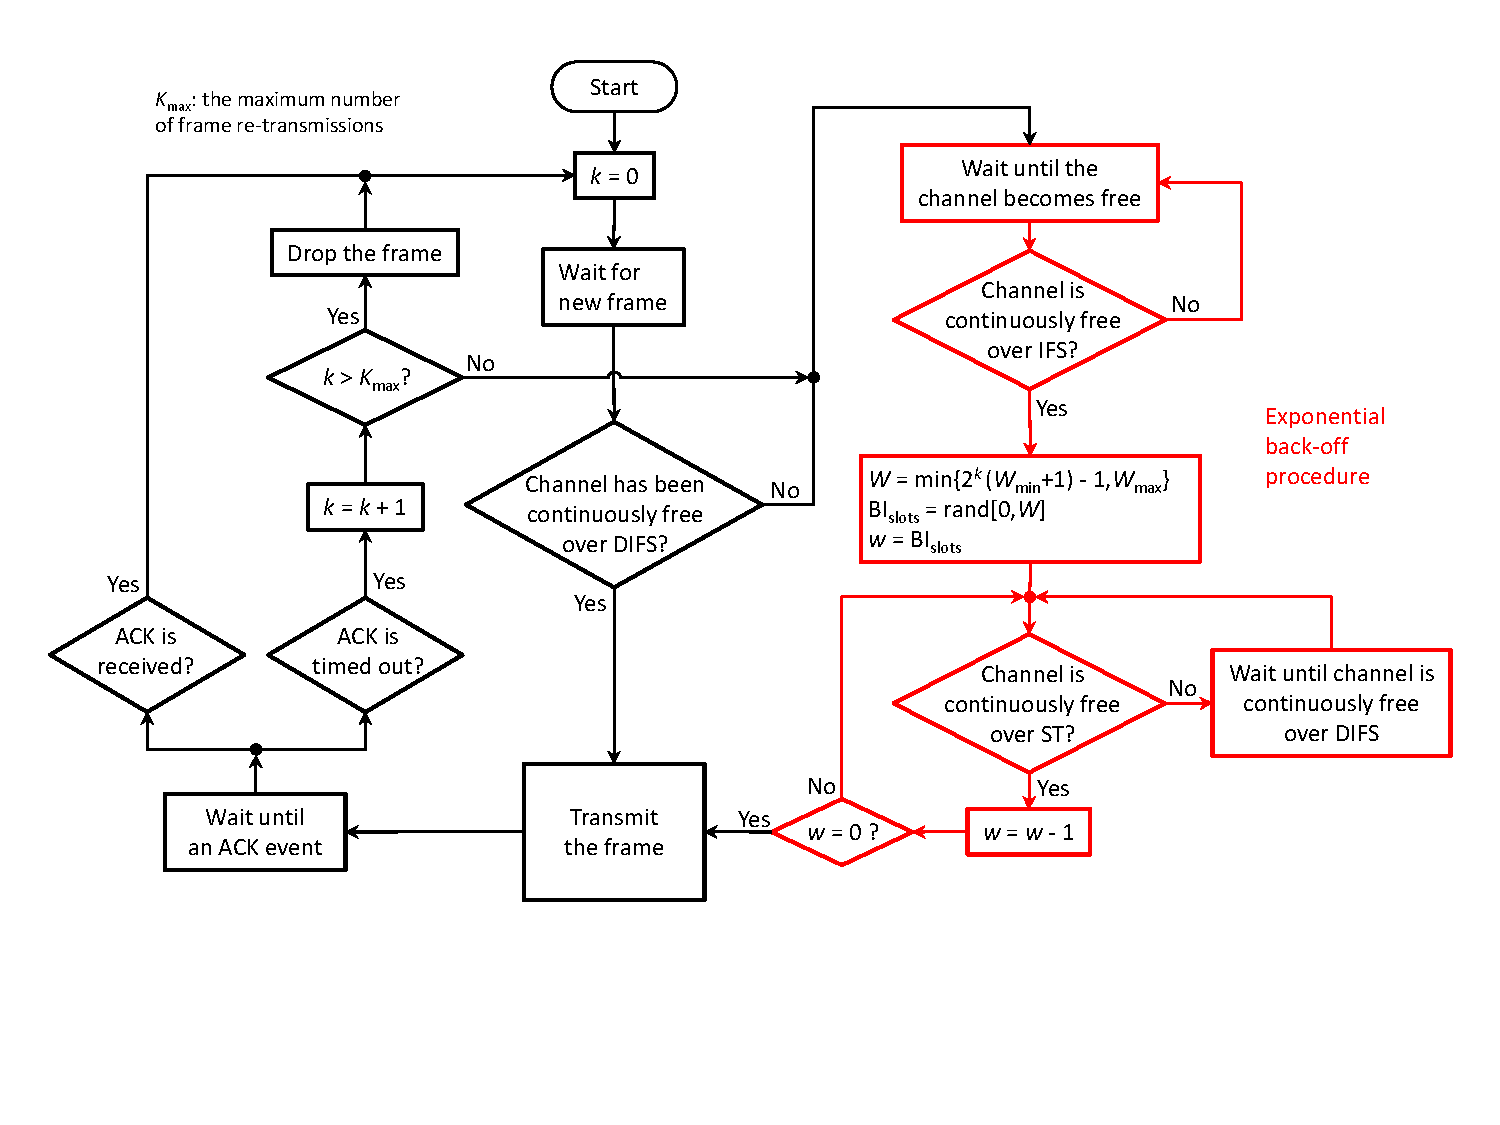
\includegraphics[width=1.0\columnwidth]{figures2/CSMA-CA-flowchart}
	\caption{Simplified flowchart of CSMA-CA.}
	\label{figs:CSMA-CA-flowchart}
\end{figure}

\subsection{Medium Access with Collision Avoidance}
\label{collision-avoidance}
Since it is difficult to detect collisions at a wireless receiver, the IEEE 802.11 protocol tries to avoid collisions, rather than detect and recover from collisions. This means that CA mechanisms are mandated to reduce the collision probability at the points where collisions would most likely occur. Specifically, most collisions happen when the medium has become idle (as indicated by CS function) after a busy state: several STAs could have been waiting for the medium to be available again, then all transmit at the same moment the medium is detected free. This situation necessitates a ``random'' back-off procedure to resolve medium contention conflicts. Also, the use of various Inter-Frame Spaces (IFSs) helps to resolve the problem. The CSMA-CA protocol is outlined as follows.

\begin{figure}[!t]
	\centering
	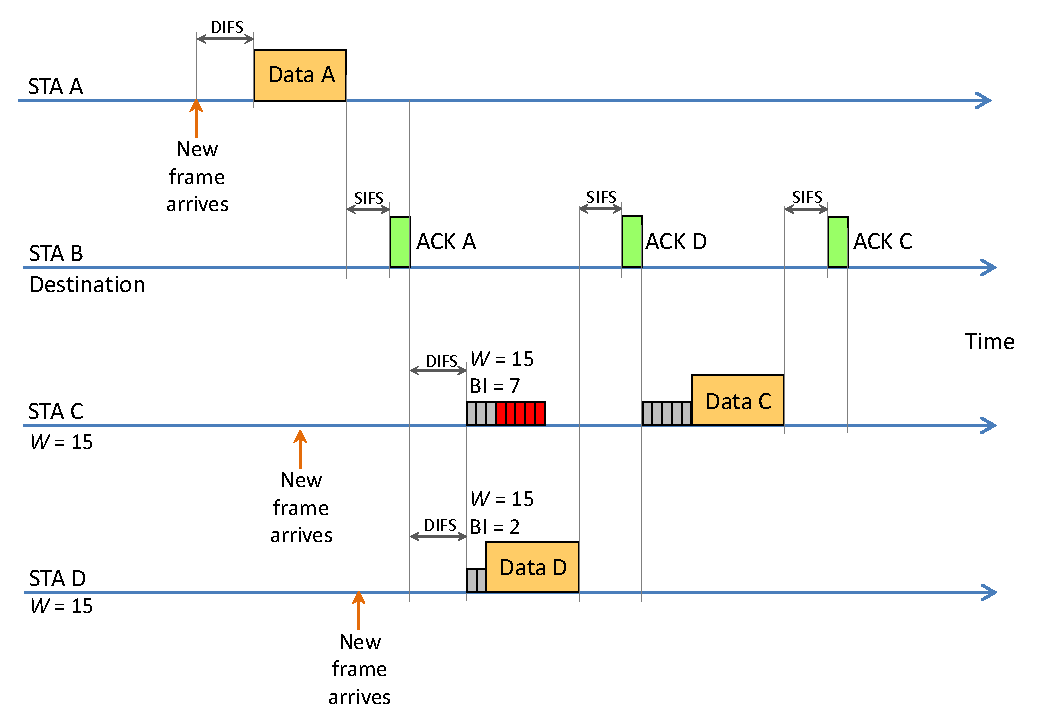
\includegraphics[width=0.9\columnwidth]{figures2/CSMA-CA-back-off-no-collision}
	\caption{CSMA-CA: An example of back-off procedure when there is no collision.}
	\label{figs:CSMA-CA-back-off-no-collision}
\end{figure}

When a STA needs to transmit a new frame, if the channel has been continuously free over a Distributed IFS (DIFS) interval, it transmits immediately. Otherwise, STA defers its transmission until the channel becomes available. Then if the channel is detected to be continuously free over a Distributed IFS (DIFS) interval, the STA will initiate the back-off procedure to further defer its transmission over a random time interval. The back-off procedure starts with the selection of a random ``slotted'' back-off interval $\mathrm{BI_{slots}} = \mathrm{rand}[0,W]$, where $\mathrm{rand}[0,W]$ is a random number uniformly distributed in the range from $0$ to $W$, $W$ is back-off window (when the system is started $W$ is assigned to its minimum value $W_{\min}$). Next, back-off counter $w$ is initialized with $\mathrm{BI_{slots}}$ and decreased every time the medium is idle over a Slot Time (ST). This counter is frozen when a transmission is detected on the medium, and resumed when the channel is detected idle again for a DIFS interval. As soon as $w$ finally reaches zero, the STA transmits its frame. It is important to note that this back-off procedure randomizes the channel access among STAs and thus helps to reduce the chance of collision. It also gives all STAs their fair shares of the channel.

The destination STA, upon receiving a frame correctly, waits for a Short IFS (SIFS) interval immediately after the reception has completed and transmits an ACK frame back to the source STA in order to confirm the correct reception. SIFS is the smallest IFS to give the highest priority channel access to ACK frames. If the source STA receives a confirmation, transmissions of the second and subsequent frames of a fragment burst will use SIFS instead of DIFS. Otherwise, the source STA activates the re-transmission procedure for the lost frame.

When a transmission is lost (due to channel collision when two or more STAs decrease their back-off counter to zero at the same time and transmit their frames at the same time or transmission errors), the contention window $W$ is doubled and applied for the re-transmissions until it reaches a maximum value $W_{\max}$. For the re-transmissions, the back-off procedure is activated after the channel remains idle for an Extended IFS (EIFS) interval. When a frame transmission is successful, contention window $W$ is reset to its minimum value $W_{\min}$. When a maximum number of frame re-transmissions is exhausted, the frame is discarded and $W$ is also reset to its minimum value $W_{\min}$.

\begin{figure}[!t]
	\centering
	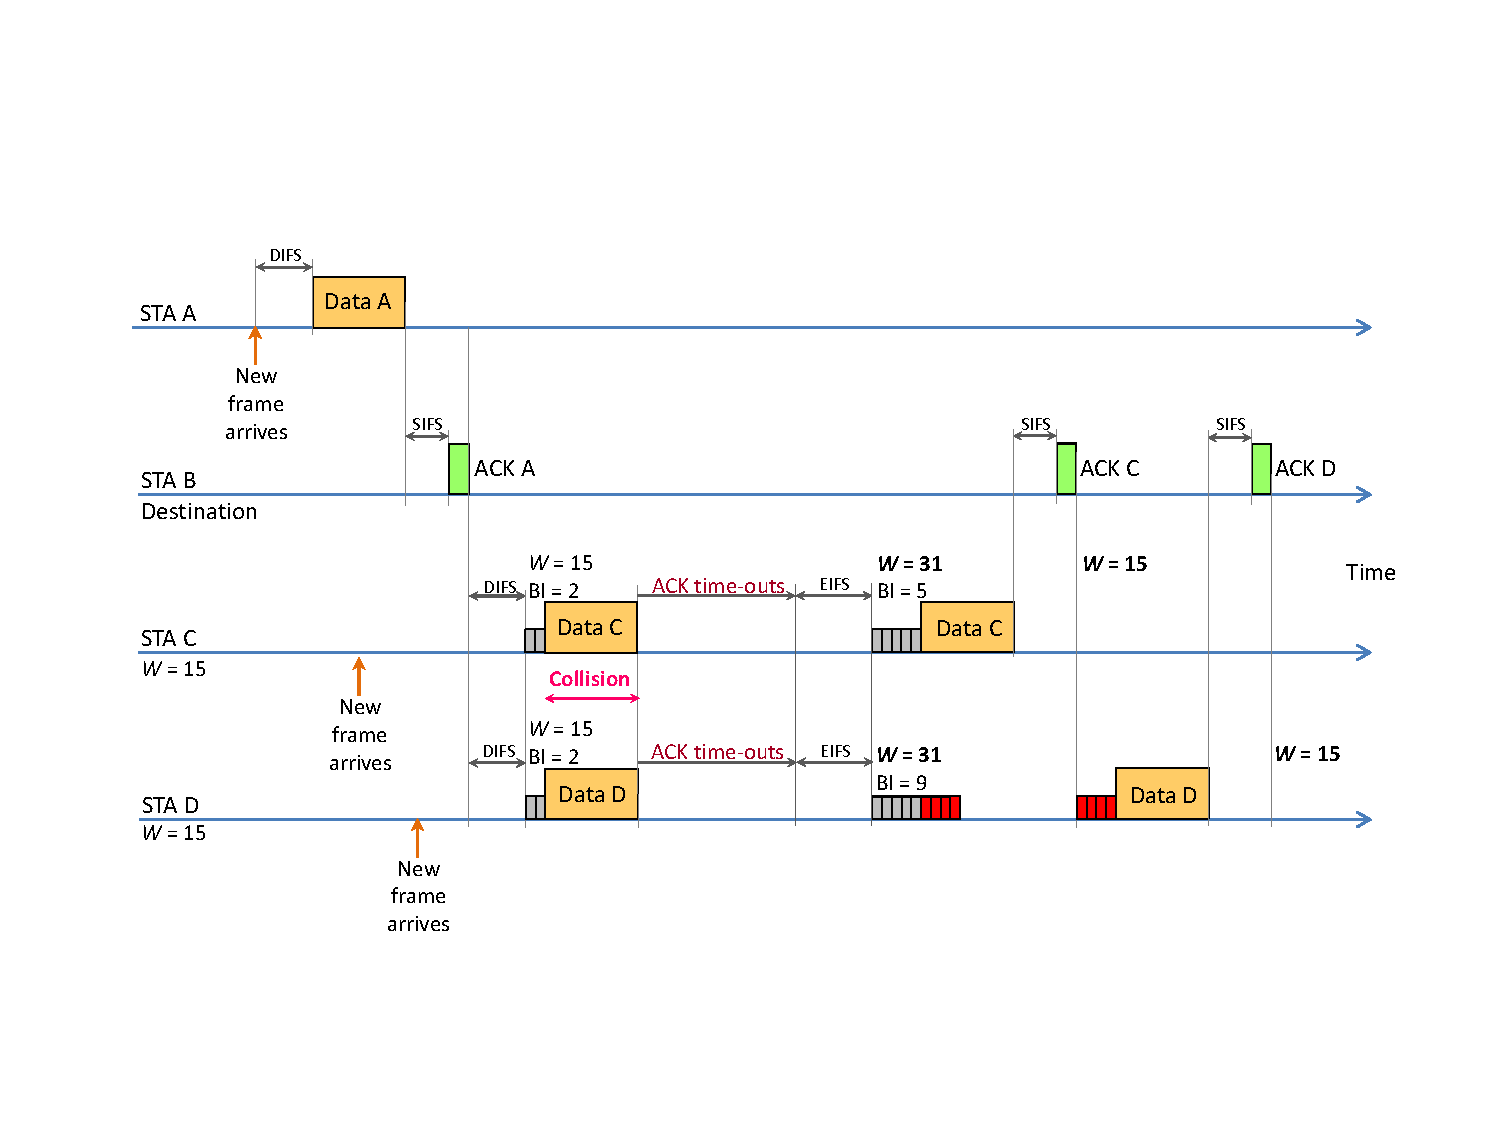
\includegraphics[width=1.0\columnwidth]{figures2/CSMA-CA-back-off-with-collision}
	\caption{CSMA-CA: An example of back-off procedure when there is a collision (the contention window is exponentially increased).}
	\label{figs:CSMA-CA-back-off-with-collision}
\end{figure}

The reason behind the exponential growth of contention window $W$ is explained as follows. When a STA experiences a collision, it has no information on how many STAs are involved in the collision. If there are only few colliding frames, it would make sense to choose the random back-off interval from a small set of small values, i.e., $W$ is small. But if many STAs are involved in a collision, then it makes sense to choose the back-off interval from a larger, more dispersed set of values, i.e., $W$ is large. Otherwise, if several STAs select the back-off interval from a small set of values, more than one STA would choose the same back-off value with high probability. This will result in high probability of collision.

Fig. \ref{figs:CSMA-CA-flowchart} shows the flowchart of CSMA-CA protocol. Figs. \ref{figs:CSMA-CA-back-off-no-collision} and \ref{figs:CSMA-CA-back-off-with-collision} demonstrates the operations of the back-off procedure in two typical scenarios. As visualized in Fig. \ref{figs:CSMA-CA-back-off-no-collision}, by randomly selecting back-off intervals, STAs C and D randomize their channel access to minimize the chance that they transmit their frames at the same time. In case a collision takes place, as shown in Fig. \ref{figs:CSMA-CA-back-off-with-collision}, STAs C and D double their contention windows to further increase the randomness in their back-off interval generations.

Here are some illustrative values of CSMA-CA operation parameters: ST = $20$ $\mu$s, SIFS = $10$ $\mu$s, DIFS = SIFS + $2\times$ST = $50$ $\mu$s, EIFS = Transmission time of ACK frame at lowest physical mandatory rate + SIFS + DIFS, $W_{\min}$ = $31$, and $W_{\max}$ = $1023$. Contention window of the initial transmission attempt is $W(0)=W_{\min}=31$. Contention window of the $k$-th re-transmission is $W(k)=\min\{2^{k}(W_{\min}+1)-1, W_{\max}\}$, where $k \in \{1,2, ..., K_{\max}\}$, $K_{\max}$ is the maximum number of re-transmission attempts. Assuming $K_{\max}=7$, then the progression of contention window with frame transmission/re-transmissions is as follows: $W(0)=31$ (the initial transmission attempt), $W(1)=63$ (the first re-transmission attempt), $W(2)=127$ (the second re-transmission attempt), $W(3)=255$ (the third re-transmission attempt), $W(4)=511$, $W(5)=1023$, $W(6)=1023$, and finally $W(7)=1023$. Different IEEE 802.11 physical layer standards could specify different values for these parameters to optimize their operations.

\begin{figure}[!t]
	\centering
	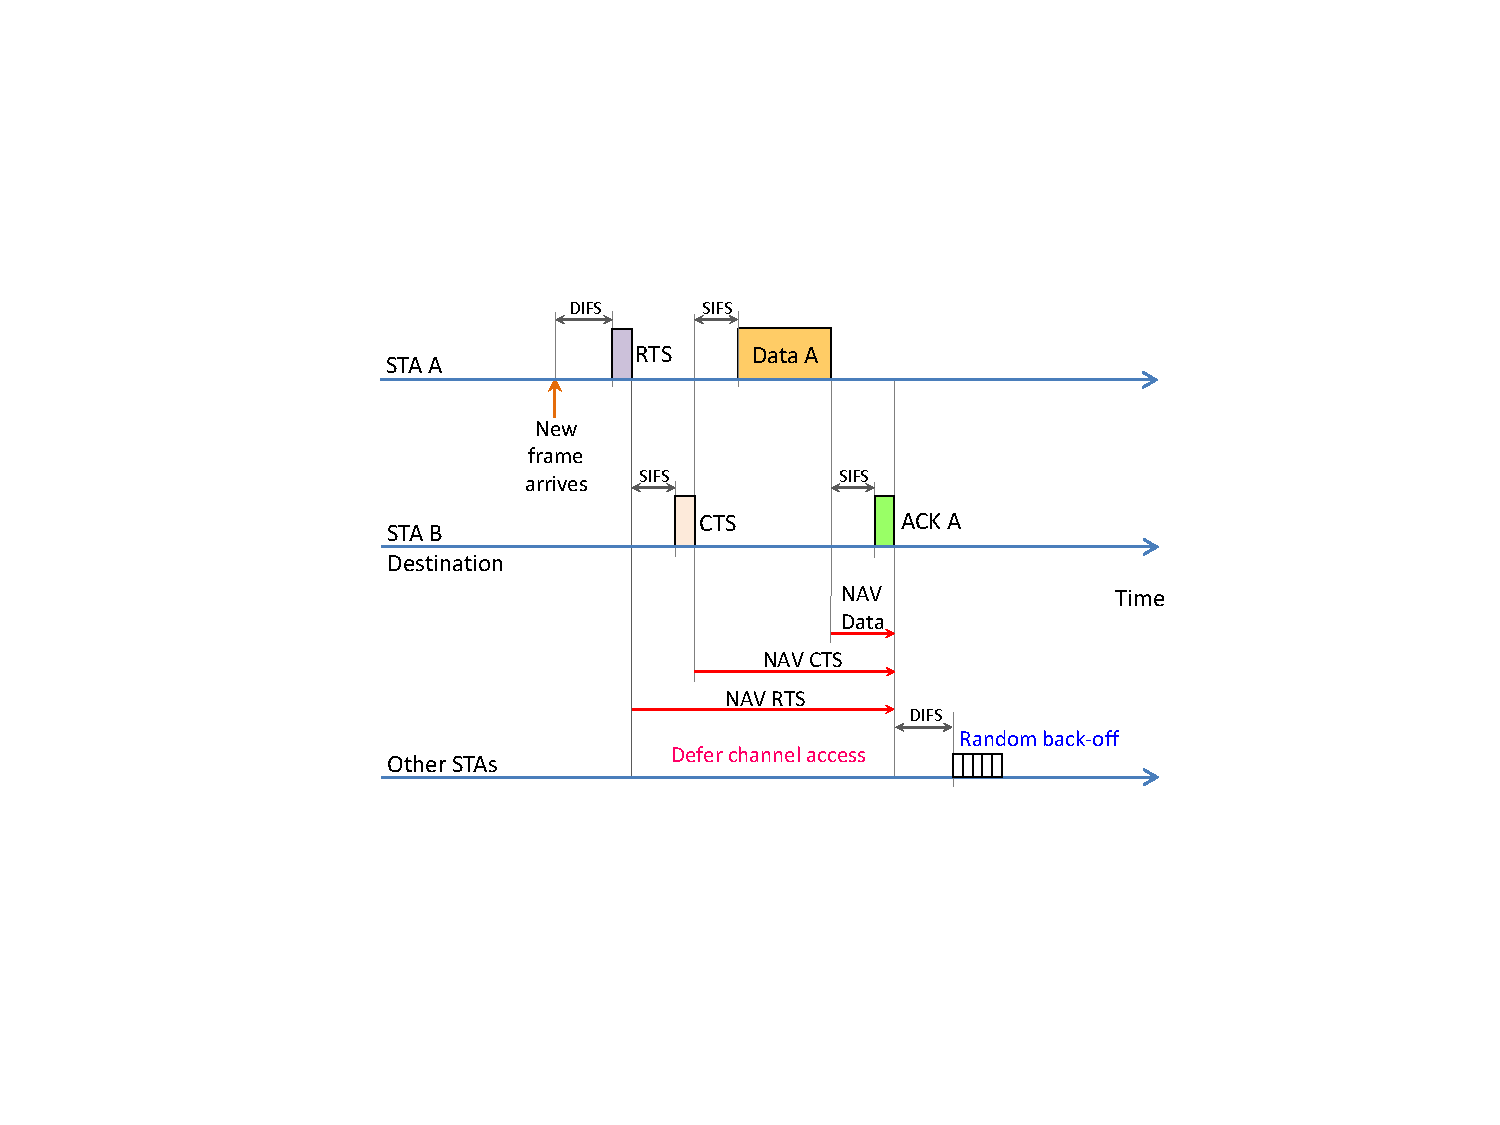
\includegraphics[width=0.65\columnwidth]{figures2/802-11-RTS-CTS-NAV}
	\caption{CSMA-CA enhanced with RTS/CTS handshake and NAV.}
	\label{figs:802-11-RTS-CTS-NAV}
\end{figure}

In order to provide guaranteed reservation of the channel and hence uninterrupted data transmission, CSMA-CA protocol can be enhanced with Request-To-Send (RTS)/Clear-To-Send (CTS) handshake and virtual carrier sense using Network Allocation Vector (NAV). The former is an optional mechanism and only employed for transmissions of long frames (determined by RTS threshold which is typically around $500$ bytes). The latter is a prominent mechanism which is widely used with CSMA-CA protocol.

In RTS/CTS access mode, prior to the data transmission, the source STA will send a RTS frame to announce the upcoming transmission. When the destination STA receives RTS, it will send a CTS frame after a SIFS interval if it is available to receive the data. The source STA is allowed to transmit its data frame only if it receives the CTS frame correctly. The purpose of this RTS/CTS exchange is to clear hidden areas and avoid long collisions. RTS/CTS is illustrated in Fig. \ref{figs:802-11-RTS-CTS-NAV}.

To implement virtual carrier sensing, each STA sends duration information in frame headers. This duration information indicates the amount of time (in microseconds) the medium is to be reserved after the end of the current frame. STAs listening on the wireless medium read the duration fields and set their NAVs, which is an indicator for a STA on how long it must defer from accessing the medium. They count down their NAVs and do not access the channel (even if their physical carrier sense indicates that the channel is free) until NAVs reach zero. NAV is illustrated in Fig. \ref{figs:802-11-RTS-CTS-NAV}. As can be seen, the NAV field in RTS frame allows CTS, data, and ACK frames to be completed (or allows only CTS frame to be completed in some implementations). The NAV in CTS frame allows data and ACK frames to be completed. Finally, the NAV in data frame allows the ACK frame to be completed.

%TODO: While all text was copied from the previous .tex file, I was not sure what went where for this subsection (and not clear what went into QoS provisioning Mechanisms)
\section{IEEE 802.11e EDCA}
\label{80211e}
The enhancement to DCF, namely Enhanced Distribution Coordination Function (EDCF), introduces the concept of access categories (ACs). Each STA has four kinds of ACs that define four respective priority levels to differentiate the channel access probability for different traffic types. With EDCF, high priority traffic has a higher chance of being sent than low priority traffic: a STA with high priority traffic waits a little less before it sends its packet, on average, than a STA with low priority traffic. This is accomplished by using a shorter contention window and shorter Arbitration Interframe Space (AIFS).

IEEE 802.11e extends the polling mechanism of PCF with the Hybrid Coordination Function (HCF). The HCF controlled channel access (HCCA) works similarly to PCF. However, in contrast to PCF, in which the interval between two beacon frames is strictly divided into two periods of CFP and CP, the HCCA allows CFPs to be initiated at almost any time during a CP. This kind of CFP is called a Controlled Access Phase (CAP) in 802.11e. A CAP is initiated by the AP whenever it wants to send a frame to a STA or receive a frame from a STA in a contention-free manner. In fact, the CFP is a CAP too. During a CAP, the Hybrid Coordinator (HC), which is also the AP, controls the access to the medium using polling mechanism. During the CP, all STAs function in EDCA. The second difference with PCF is that Traffic Class (TC) and Traffic Streams (TSs) are defined. This means that HC is not limited to per-station queuing and can provide a kind of per-session service. Also, HC can coordinate these streams or sessions in any fashion it chooses (not just round robin). Moreover, STAs give information about the lengths of their queues for each TC. HC can use this information to give priority to one STA over another, or better adjust its scheduling mechanism.

IEEE 802.11e additionally introduces the concept of transmission opportunity (TXOP). A STA which obtains medium access must not utilize radio resource for duration longer than a limit specified by TXOP. The use of TXOPs reduces the problem of low-rate STAs gaining an inordinate amount of channel time in the conventional 802.11 DCF MAC. Another enhancement is that a STA is only allowed to initiate a frame exchange if it can complete the exchange before the start of the next beacon interval.
\subsection{QoS Provisioning Mechanisms}
\label{qos}

\subsection{EDCA and HCCA}
\label{edca-hcca}
Basic operations of HCCA are illustrated in Fig. \ref{figs:802-11e-HCCA}. HCCA is generally considered as the most advanced and complicated coordination function. With HCCA, QoS can be configured with great precision. QoS-enabled STAs have the ability to request specific transmission parameters (data rate, jitter, etc.), which should allow advanced applications like voice over IP (VoIP) and video streaming to work more effectively on Wi-Fi networks. However, due to its complexity and signaling overhead, HCCA has not been widely implemented.

It can be seen IEEE 802.11 CSMA-CA is the most fundamental protocol for medium access in WLANs. In fact, IEEE 802.11e EDCA is primarily designed based on CSMA-CA. As a result, in-depth knowledge on medium access mechanisms employed by this protocol is imperative to unde
\begin{figure}[!t]
	\centering
	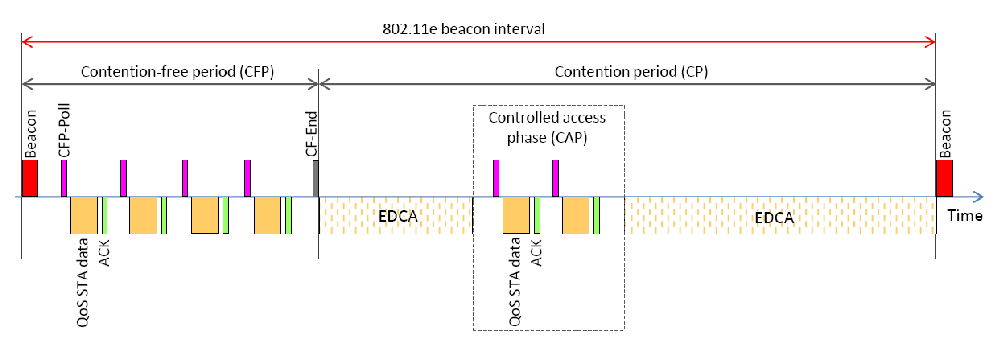
\includegraphics[width=1.0\columnwidth]{figures2/802-11e-HCCA}
	\caption{HCCA in IEEE 802.11e.}
	\label{figs:802-11e-HCCA}
\end{figure}

\section{Important Observations on CSMA-CA}
\label{csmaca-obs}
It is important to note that IEEE 802.11 CSMA-CA is specified with a few key additional features that go beyond LBT requirements specified by ETSI \cite{LBT-ETSI-2014}. \textit{First}, a Wi-Fi device defers to signals that are much weaker than the minimum level required by ETSI. ETSI LBT requires a transmitter to defer if the received energy is above $-60$ dBm (for $20$ MHz), while Wi-Fi defers if the received energy is above $-62$ dBm (this level is referred to as the energy detect threshold, or ED for short) or if a valid Wi-Fi preamble is detected. Wi-Fi's ED threshold is nearly the same as ETSI's LBT threshold, but Wi-Fi preamble detection is required to work to at least $-82$ dBm, and in reality works to $-90$ dBm or lower in most products. Hence, Wi-Fi devices defer to other Wi-Fi transmissions much more conservatively (i.e., at a much larger distance) than a device which only meets ETSI requirements. \textit{Second}, Wi-Fi goes beyond the ETSI requirements in specifying how long a device must wait after the on-air energy falls below the threshold before initiating a transmission. \textit{Third}, when a collision is detected, Wi-Fi employs exponential back-off rule that doubles the contention window size and thus significantly increases the random back-off time in order to avoid future collision.

%%%%%%%%%%%%%%%%%%%%%%%% referenc.tex %%%%%%%%%%%%%%%%%%%%%%%%%%%%%%
% sample references
% %
% Use this file as a template for your own input.
%
%%%%%%%%%%%%%%%%%%%%%%%% Springer-Verlag %%%%%%%%%%%%%%%%%%%%%%%%%%

\begin{thebibliography}{99.}%
\bibitem{wifi-alliance}``Wi-Fi® device shipments to surpass 15 billion by end of 2016'', Online, {Wi-Fi}  Alliance. Available:  \url{{ttp://www.wi-fi.org/news-events/newsroom/wi-fi-device-shipments-to-surpass-15-billion-by-end-of-2016}}.
\bibitem{80211}``{IEEE Standard for information technology--Telecommunications and information exchange between systems Local and metropolitan area networks--Specific requirements Part 11: Wireless LAN medium access control (MAC) and Physical Layer (PHY) specifications},'' \emph{{IEEE Std 802.11-2012 (Revision of IEEE Std 802.11-2007)}}, March 2012.
\bibitem{80211ac}``{IEEE Standard for information technology--Telecommunications and information exchange between systems Local and metropolitan area networks--Specific requirements Part 11: Wireless LAN medium access control (MAC) and Physical Layer (PHY) specifications}--Amendment 4: Enhancements for very high throughput for operation in bands below 6 GHz,'' \emph{{IEEE Std 802.11ac-2013 (Revision of IEEE Std 802.11-2007)}}, December 2013.
\bibitem{80211ad}``{IEEE Standard for information technology--Telecommunications and information exchange between systems Local and metropolitan area networks--Specific requirements Part 11: Wireless LAN medium access control (MAC) and Physical Layer (PHY) specifications amendment 3: Enhancements for very high throughput in the 60 GHz band},'' \emph{{IEEE Std 802.11ad-2012 }},  December 2012.
\bibitem{ieee-history}{J. Berg}, ``The  IEEE  802.11  standardization  – Its  history,  specifications,  implementations,  and  future''; TechnicalReport GMU-TCOM-TR-8,  George  Mason  University. 
Available: \url{\text{http://telecom.gmu.edu/sites/default/files/publications/Berg\_802.11\_GMU-TCOM-TR-8.pdf}}.
\bibitem{LBT-ETSI-2014} \emph{ETSI EN 301 893 V1.7.2 (2014-07): Broadband radio access networks (BRAN);	5 GHz high performance RLAN; Harmonized EN covering the essential requirements of article 3.2 of the R\&TTE Directive}, European Telecommunications Standards Institute Std., 2014.
\end{thebibliography}
%%%%%%%%%%%%%%%%%%%%% chapter.tex %%%%%%%%%%%%%%%%%%%%%%%%%%%%%%%%%
%
% sample chapter
%
% Use this file as a template for your own input.
%
%%%%%%%%%%%%%%%%%%%%%%%% Springer-Verlag %%%%%%%%%%%%%%%%%%%%%%%%%%
%\motto{Use the template \emph{chapter.tex} to style the various elements of your chapter content.}
\chapter{U-LTE and Wi-Fi Coexistence: A Survey}
\label{survey} % Always give a unique label
% use \chaptermark{}
% to alter or adjust the chapter heading in the running head

\abstract*{Coexistence between \mbox{U-LTE} and \mbox{Wi-Fi} networks is a deciding factor on the acceptance of \mbox{U-LTE}. As a result, a large number of studies have been carried out to identify what could be the affects that \mbox{U-LTE} may cause to \mbox{Wi-Fi} and which mechanisms could be used for ensure that these two technologies share the $5$ GHz unlicensed frequency band in an efficient and fair manner. This chapter presents a survey on related work to answer the following questions: (i) what issues arise from simultaneous operation of LTE and \mbox{Wi-Fi} in the same spectrum bands, (ii) which technology is affected the most, and (iii) which factors determine the impacts of \mbox{U-LTE} to \mbox{Wi-Fi}. It also identifies the strengths and weaknesses of existing solutions and suggests potential strategies to improve performance of these two technologies.}

Coexistence between \mbox{U-LTE} and \mbox{Wi-Fi} networks is a deciding factor on the acceptance of \mbox{U-LTE}. As a result, a large number of studies have been carried out to identify what could be the affects that \mbox{U-LTE} may cause to \mbox{Wi-Fi} and which mechanisms could be used for ensure that these two technologies share the $5$ GHz unlicensed frequency band in an efficient and fair manner. This chapter presents a survey on related work to answer the following questions: (i) What issues arise from simultaneous operation of LTE and \mbox{Wi-Fi} in the same spectrum bands?; (ii) Which technology is affected the most?; and (iii) Which factors determine the impacts of \mbox{U-LTE} to \mbox{Wi-Fi}? The strengths and weaknesses of existing solutions and potential strategies to improve performance of these two technologies are also identified.

\section{Impacts of U-LTE on Wi-Fi Operation and Performance}

In \cite{original-LTE-Wi-Fi-VTC-2013}, extensive simulations were performed to assess the performance of LTE and \mbox{Wi-Fi} when the technologies are coexisting in an office environment. Both single-floor and multi-floor office environments, with different assumptions as to the density of \mbox{Wi-Fi} and LTE nodes, have been considered. The simulation results show that, in the absence of any modification to the LTE channel access mechanism, channel sharing between LTE and \mbox{Wi-Fi} networks is significantly unfair for \mbox{Wi-Fi} networks. While LTE experience only marginal performance loses when \mbox{Wi-Fi} is present on the same band (about $4$\% from the baseline performance), in a sparse deployment of $1$ AP per system per floor, \mbox{Wi-Fi} could lose up to $70$\% compared to its baseline performance.  In a dense deployment of $5$ APs per system per floor, the losses seen by \mbox{Wi-Fi} were nearly $100$\%. Detailed investigations in \cite{original-LTE-Wi-Fi-VTC-2013} indicate that for \mbox{Wi-Fi} the channel is blocked when LTE interference is present, and thus \mbox{Wi-Fi} nodes remain in ``listen'' for a clear channel mode most of the time.

The authors in \cite{original-LTE-Wi-Fi-WCNC-2013} present observations similar to those in \cite{original-LTE-Wi-Fi-VTC-2013} on the effects of unmodified LTE on the performance of \mbox{Wi-Fi} networks sharing the same frequency band. Specifically, it was found that as network load is increased LTE performance suffers only a minor degradation while \mbox{Wi-Fi} performance drops significantly. These results can be explained by the increasing LTE occupancy on the shared band because LTE does not follow the same rules as \mbox{Wi-Fi} in shared medium access. When there is ongoing transmission on the channel, \mbox{Wi-Fi} politely defers its transmissions while LTE will always choose to transmit and simply select a more robust transmission mode by adapting its modulation and channel coding scheme in order to cope with the higher levels of interference. This aggressive behavior quickly results in a situation where LTE terminals take all transmission opportunities while \mbox{Wi-Fi} devices are locked in defer and back-off procedures. Fortunately, the results in \cite{original-LTE-Wi-Fi-WCNC-2013} have also demonstrated that the severity of this negative impact on \mbox{Wi-Fi} can be efficiently controlled by restricting LTE activity.

The authors in \cite{LTE-U-PIMRC-2014} analyze the performance degradation of \mbox{Wi-Fi} in the presence of \mbox{LTE-U} with the probability of \mbox{Wi-Fi} accessing the channel is used as the main metric. Numerical results indicate that \mbox{Wi-Fi} is negatively affected by conventional LTE operation due to LTE's almost continuous transmissions subsequently blocking \mbox{Wi-Fi} access. Specifically, given the two modes of operations currently proposed for \mbox{LTE-U} in the unlicensed spectrum, the ``off'' period presented by the LTE protocol is too short for \mbox{Wi-Fi} users to access the channel. As a result, \mbox{Wi-Fi} is at risk of spending a significant amount of time in the ``listening'' mode when LTE transmissions are present in the same channel.

The work in \cite{U-LTE-Google-WP} presents initial investigations on the coexistence of two versions of license-anchored \mbox{U-LTE} (i.e., \mbox{LTE-U} and \mbox{LAA-LTE}) and \mbox{Wi-Fi} in $5$ GHz frequency band. Results show that \mbox{LTE-U} poorly coexists with \mbox{Wi-Fi} primarily due to two factors: (i) the incompatibility of \mbox{LTE-U}'s duty-cycling mechanism with \mbox{Wi-Fi} equipment and (ii) the lack of an effective coexistence mechanism in scenarios where \mbox{LTE-U} and \mbox{Wi-Fi} devices hear each other at moderate but non-negligible power levels. Additionally, \mbox{LAA-LTE} with LBT does not by itself guarantee successful fair coexistence with \mbox{Wi-Fi}. The results in \cite{U-LTE-Google-WP} were submitted to the FCC in June 2015 to demonstrate that, although any wireless technology should have the ability to utilize unlicensed spectrum within the FCC's rules, \mbox{U-LTE} has the potential to crowd out unlicensed services.

An experiment-based study on the effect of \mbox{LTE-U} to \mbox{Wi-Fi} is presented in \cite{LTE-U-CableLabs}. The LTE signal level was set higher than the \mbox{Wi-Fi} clients' LBT energy detection threshold (i.e., when LTE is on, the \mbox{Wi-Fi} client should sense their presence and not transmit). \mbox{Wi-Fi} throughput and latency were measured when data is transmitted through the \mbox{Wi-Fi} network with varying duty cycles and periods of LTE signals. The results in \cite{LTE-U-CableLabs} indicate that, as expected, increasing the \mbox{LTE-U} duty cycle degrades both \mbox{Wi-Fi} throughput and latency performance since it decreases \mbox{Wi-Fi} transmission opportunities accordingly. If the duty cycle period is too high, \mbox{Wi-Fi} latency is negatively impacted (while \mbox{Wi-Fi} throughput is nearly unchanged, given the same duty cycle) since \mbox{Wi-Fi} frames have to be buffered during long LTE ``on'' period. However, if the duty cycle period is configured as too low (e.g., $10$ msec), \mbox{Wi-Fi} throughput degrades due to the fact that LTE ``on'' and ``off'' periods are too short for \mbox{Wi-Fi} users to both access the channel and complete their transmissions. Furthermore, the authors in \cite{LTE-U-CableLabs} indicate that \mbox{LTE-U} duty cycle cannot strictly results in corresponding air time and throughput sharings. For example, with a duty cycle of $50$\%, \mbox{LTE-U} is likely to capture more than $50$\% of the channel resources. The reason is that when \mbox{LTE-U} starts its transmissions (regardless of ongoing \mbox{Wi-Fi} frame transmissions), many \mbox{Wi-Fi} frames are corrupted. The resulting transmission failures lead to multiple frame re-transmissions and, more importantly, mistakenly force \mbox{Wi-Fi} transceivers to operate at lower rates (in this case, lowering the channel coding and modulation modes is not necessary and is a waste of channel efficiency).


\section{Existing Solutions to Address the U-LTE and Wi-Fi Coexistence Concern}

Various coexistence mechanisms proposed for \mbox{U-LTE} are surveyed in \cite{U-LTE-survey-2014, U-LTE-survey-2015, U-LTE-5G-2015}. The proposed mechanisms include: Dynamic Channel Selection (DCS), transmission power control, opportunistic secondary cell ``off'', CSAT (in \mbox{LTE-U}), and LBT (in \mbox{LAA-LTE}). When \mbox{U-LTE} and \mbox{Wi-Fi} share the common $5$ GHz radio frequency band, those mechanisms are found to be useful to reduce RFI and improve the spectrum utilization efficiency. However, the roles and performance of each varies greatly depending on network and system parameters including network scale, node density, deployment and radio environment (i.e., indoor, outdoor, short range, long range, etc.), and network load profiles. 

In order to see how LBT mechanisms employed by \mbox{LAA-LTE} can help promote fair coexistence, a simulation-based study is carried out and reported in \cite{LBT-CableLabs-2014}. LBE LBT specified by ETSI \cite{LBT-ETSI-2014} and IEEE 802.11e Enhanced Distributed Channel Access (EDCA) are assumed for \mbox{LAA-LTE} and \mbox{Wi-Fi}, respectively. The most important observation from \cite{LBT-CableLabs-2014} is that LBT compliant to ETSI regulation is not sufficient for fair coexistence: \mbox{Wi-Fi} STAs have much lower probability of successful channel access compared to \mbox{LAA-LTE} users. One major reason for this phenomenon is the non-exponential back-off employed by \mbox{LAA-LTE} LBT. Unfortunately, no form of exponential back-off LBT is studied in \cite{LBT-CableLabs-2014}.

In \cite{U-LTE-Wi-Fi-Qualcomm-2014, LTE-U-Wi-Fi-LTE-U-Forum-2015, LTE-U-Qualcomm-2015, U-LTE-Wi-Fi-Qualcomm-FCC-2015}, the performance of \mbox{LTE-U} and \mbox{LAA-LTE} and \mbox{Wi-Fi} in a shared frequency band is evaluated. DCS and opportunistic secondary cell ``off'' in unlicensed spectrum (\mbox{U-LTE} small cells would release the unlicensed carriers and fall back to the anchor carrier in licensed spectrum at low traffic load) are jointly used with CSAT and LBT. The results show that coexistence has a negative but controllable impact on \mbox{Wi-Fi} performance. In \cite{U-LTE-Wi-Fi-Qualcomm-2014, LTE-U-Wi-Fi-LTE-U-Forum-2015, LTE-U-Qualcomm-2015}, \mbox{LTE-U} can be a better neighbor to \mbox{Wi-Fi} than \mbox{Wi-Fi} would be to itself, in some scenarios. The underlying design that allows \mbox{LTE-U} to achieve high spectral efficiency while being a good neighbor to \mbox{Wi-Fi} is achieved through a set of carefully designed coexistence techniques, including DCS, secondary cell ``duty cycle'' in unlicensed spectrum (i.e., CSAT), and opportunistic secondary cell ``off'' in unlicensed spectrum. Specifically, in scenarios where the density of \mbox{Wi-Fi} APs and small cells is low or moderate, DCS and opportunistic secondary cell ``off'' are sufficient to meet the coexistence requirement. When \mbox{LTE-U} devices replace \mbox{Wi-Fi} devices, they can achieve significantly higher throughputs due to their high spectral efficiency. In addition, the performance of neighboring \mbox{Wi-Fi} is unchanged or even slightly improved since \mbox{LTE-U} devices can finish transmissions faster, and incur less interference, the similarly deployed \mbox{Wi-Fi} APs. However, if the density of \mbox{Wi-Fi} devices and \mbox{LTE-U} small cells is high, DCS and opportunistic secondary cell ``off'' alone cannot guarantee harmonious coexistence with \mbox{Wi-Fi} and therefore CSAT or LBT is required. Resutls in \cite{LTE-U-Wi-Fi-LTE-U-Forum-2015, U-LTE-Wi-Fi-Qualcomm-FCC-2015} were submitted to the FCC in 2015 to support \mbox{U-LTE} technologies.

A systematic and large-scale network-wide study of \mbox{LAA-LTE} and \mbox{Wi-Fi} performance in a wide range of realistic deployment scenarios and network densities in the unlicensed $5$ GHz band is presented in \cite{LTE-U-ICC-WS-2015}. The simulation results in all considered coexistence scenarios demonstrate that both \mbox{LAA-LTE} and \mbox{Wi-Fi} significantly benefit from the large number of available channels and the isolation provided by building shielding at $5$ GHz. They also suggest that deploying \mbox{LAA-LTE} with a random channel selection scheme is feasible for lower network densities. For typical indoor deployments of high density, implementing \mbox{LTE-U} interference-aware channel selection with respect to \mbox{Wi-Fi} is superior to LBT in terms of achieved throughput for both technologies. Additionally, LBT can increase \mbox{LAA-LTE} user throughput when multiple outdoor \mbox{LAA-LTE} networks deployed by different cellular operators coexist.

The work in \cite{Enhanced-LTE-U-thesis-2015} investigates the behavior and performance of two existing LBT mechanisms that are designed following the coexistence standard specified by ETSI, namely LBE- and FBE-based mechanisms \cite{LBT-ETSI-2014}. The Jain's fairness index has been used to assess the coexistence of \mbox{LAA-LTE} using these two LBT mechanisms and compare to \mbox{Wi-Fi} using CSMA-CA. The simulations in \cite{Enhanced-LTE-U-thesis-2015} show that the FBE-based mechanism, using a fixed contention window, impairs the channel access opportunity of \mbox{Wi-Fi}'s CSMA-CA using an adaptive contention window. The simulations reveal that FBE-based mechanism tends to aggressively occupy the channel. In some cases, \mbox{Wi-Fi} devices are starved with very few, or even no, chances to access the channel. This poor fairness is mainly caused by the short CCA sensing period of FBE-based mechanism. CCA is applied only once and then FBE-based mechanism may start its transmission immediately while LBE and \mbox{Wi-Fi}-based mechanisms are still decrementing their respective back-off counters. The fairness is worsened by the longer frames used by FBE. Another observation is that, again due to equal CCA sensing time, when multiple FBE-based equipment are contending for the channel, they are prone to serious collisions (if they are accidentally synchronized) or suffer a significant unfairness (if they are asynchronous). To cope with those issues, tuning the values of the back-off scaler ($q$) to extend the contention window size and using CCA procedure similar to that of LBE-based mechanism have been suggested for LBE and FBT-based mechanism, respectively. The results in \cite{Enhanced-LTE-U-thesis-2015} demonstrate that the modified LBE-based mechanism still cannot sufficiently improve the level of fairness achieved with others. This could be because simply empirically tuning the back-off scaler, while keeping the CCA principle unchanged, cannot compensate for the exponential growth of window size adopted by \mbox{Wi-Fi}'s CSMA-CA. The modified FBE-based mechanism can offer better fairness when coexisting with \mbox{Wi-Fi}.

A comparison of \mbox{LTE-U} and \mbox{LAA-LTE} is presented in \cite{LBT-CSAT-2015}. The analysis in \cite{LBT-CSAT-2015} shows that for sufficiently long LTE transmission times, the LTE throughputs achieved by CSAT and LBE are almost identical. However, for shorter LTE transmission times, \mbox{LTE-U} provides lower LTE throughput than \mbox{LAA-LTE} due to higher LTE/\mbox{Wi-Fi} collision probability of \mbox{LTE-U}. Besides, while shorter LTE transmission time decreases the tail of the \mbox{Wi-Fi} delay distribution, the percentage of packets that suffer from long delays increases. The results also indicate that when appropriately configured, \mbox{LTE-U} and \mbox{LAA-LTE} provide the same level of fairness to \mbox{Wi-Fi}. The selection of coexistence mechanisms is primarily driven by the operator's interests that include implementation complexity, LTE throughput, operational and management costs as well as strategic decisions on targeted markets.

Coordinated coexistence between \mbox{U-LTE} and \mbox{Wi-Fi} is investigated in \cite{U-LTE-5G-2015, Coordinated-LTE-U-Wi-Fi-2015}. The authors in \cite{U-LTE-5G-2015} propose a method of centralized system management which combines \mbox{LTE-U} and \mbox{Wi-Fi} through network function virtualization (NFV) interconnections. This technique may enable seamless transfers of resources between \mbox{LTE-U} and \mbox{Wi-Fi} using in-the-cloud control of distributed APs. However, only \textit{conceptual} network architectures and mechanisms are presented. The authors in \cite{Coordinated-LTE-U-Wi-Fi-2015} present a Software Defined Networking (SDN) architecture to support logically-centralized dynamic spectrum management involving multiple autonomous networks to improve spectrum utilization and facilitate coexistence. The basic design goal is to support the seamless communication and information dissemination required for coordination of heterogeneous networks. The system consists of two-tiered controllers mainly responsible for the control plane. The Global Controller (GC) acquires and processes global network state information (radio coverage maps, coordination algorithms, policy and network evaluation matrices, etc.) and controls the flow of information between Regional Controllers (RCs) and databases based on authentication and other regulatory policies. RCs acquire local visibility needed for radio resource allocation at wireless devices (device location, frequency band, duty cycle, power level, and data rate, etc.). Joint transmission power control and time division channel access optimizations are further proposed. Analytical results in \cite{Coordinated-LTE-U-Wi-Fi-2015} demonstrate that, \textit{with full buffer traffic assumption}, centralized optimization approaches can provide fair access to the spectrum for \mbox{LTE-U} and \mbox{Wi-Fi} networks.

An experimental evaluation of \mbox{U-LTE} interference effects on \mbox{Wi-Fi} performance under various network conditions, along with some suggestions for better coexistence of \mbox{U-LTE} and \mbox{Wi-Fi} networks, are presented in \cite{LTE-U-Experiment-ICC-WS-2015}. Various system parameters (bandwidth, center frequency, etc.) are swept to identify the most significant parameters that determine the levels of LTE interference introduced to \mbox{Wi-Fi} carrier sense and their effects on performance. The results indicate that \mbox{Wi-Fi} throughput can be heavily degraded by \mbox{LAA-LTE} transmissions with $3$/$5$/$10$ MHz bandwidth (especially $3$/$5$ MHz). Besides, \mbox{LAA-LTE} transmissions can have small impact on \mbox{Wi-Fi} throughput when using a $1.4$ MHz channel with center frequencies located on the guard bands or the center frequencies of \mbox{Wi-Fi} channels. However, the authors in \cite{LTE-U-Experiment-ICC-WS-2015} do not clearly define what \mbox{LAA-LTE} really mean in their work. It seems to be that they simply perform experiments with conventional LTE transceivers of varying power spectral densities and do not incorporate any coexistence mechanism into the LTE system.



\begin{thebibliography}{99.}%
\bibitem{U-LTE-survey-2014}F.~Abinader, E.~Almeida, F.~Chaves, A.~Cavalcante, R.~Vieira, R.~Paiva, A.~Sobrinho, S.~Choudhury, E.~Tuomaala, K.~Doppler, and V.~Sousa, ``Enabling the coexistence of {LTE} and {Wi-Fi} in unlicensed bands,'' \emph{IEEE	Communications Magazine}, vol.~52, no.~11, pp. 54--61, Nov 2014.	
	
\bibitem{U-LTE-survey-2015} H.~Zhang, X.~Chu, W.~Guo, and S.~Wang, ``Coexistence of {Wi-Fi} and heterogeneous small cell networks sharing unlicensed spectrum,'' \emph{IEEE	Communications Magazine}, vol.~53, no.~3, pp. 158--164, March 2015.

\bibitem{U-LTE-5G-2015}A.~Al-Dulaimi, S.~Al-Rubaye, Q.~Ni, and E.~Sousa, ``{5G} communications race: Pursuit of more capacity triggers {LTE} in unlicensed band,'' \emph{IEEE Vehicular Technology Magazine}, vol.~10, no.~1, pp. 43--51, March 2015.

\bibitem{original-LTE-Wi-Fi-VTC-2013}A.~M. Cavalcante \emph{et~al.}, ``Performance evaluation of {LTE} and {Wi-Fi} coexistence in unlicensed bands,'' in \emph{Proceedings of 2013 IEEE	Vehicular Technology Conference (VTC Spring)}, 2013, pp. 1--6.

\bibitem{original-LTE-Wi-Fi-WCNC-2013} T.~Nihtila, V.~Tykhomyrov, O.~Alanen, M.~Uusitalo, A.~Sorri, M.~Moisio, S.~Iraji, R.~Ratasuk, and N.~Mangalvedhe, ``System performance of {LTE} and
{IEEE} 802.11 coexisting on a shared frequency band,'' in \emph{2013 IEEE Wireless Communications and Networking Conference (WCNC)}, April 2013, pp. 1038--1043.

\bibitem{LTE-U-PIMRC-2014} A.~Babaei, J.~Andreoli-Fang, and B.~Hamzeh, ``On the impact of {LTE-U} on {Wi-Fi} performance,'' in \emph{2014 IEEE 25th Annual International Symposium	on Personal, Indoor, and Mobile Radio Communication (PIMRC)}, Sept 2014, pp.1621--1625.

\bibitem{U-LTE-Google-WP} N.~Jindal and D.~Breslin, ``{LTE} and {Wi-Fi} in unlicensed spectrum: A coexistence study,'' white paper, Google.

\bibitem{LTE-U-CableLabs} J.~Padden, ``{Wi-Fi} vs. duty cycled {LTE}: A balancing act,'' CableLabs. [Online]. Available: \url{http://www.cablelabs.com/wi-fi-vs-duty-cycled-lte/}

\bibitem{LBT-CableLabs-2014} J.~P. A.~Babaei and J.~Andreoli-fang, ``Overview of {EU} {LBT} and its effectiveness for coexistence of {LAA LTE} and {Wi-Fi},'' IEEE 802.19-14/0082r0, CableLabs, Nov. 2014.

\bibitem{U-LTE-Wi-Fi-Qualcomm-2014} ``{LTE} in unlicensed spectrum: Harmonious coexistence with {Wi-Fi},'' whitepaper, Qualcomm Inc., Jun. 2014.

\bibitem{LTE-U-Wi-Fi-LTE-U-Forum-2015} ``{LTE-U} technical report: Coexistence study for {LTE-U} {SDLV1.0(2015-02)},'' LTE-U Forum, Tech. Rep., 2015.

\bibitem{LTE-U-Qualcomm-2015}A.~Sadek, T.~Kadous, K.~Tang, H.~Lee, and M.~Fan, ``Extending {LTE} to unlicensed band - merit and coexistence,'' in \emph{Communication Workshop (ICCW), 2015 IEEE International Conference on}, June 2015, pp. 2344--2349.

\bibitem{U-LTE-Wi-Fi-Qualcomm-FCC-2015}``Office of engineering and technology and wireless telecommunications bureau seek information on current trends in {LTE-U} and {LAA} technology,''
Comments of Qualcomm Incoporated, Qualcomm Inc., Jun. 2015.

\bibitem{LTE-U-ICC-WS-2015} A.~Voicu, L.~Simic, and M.~Petrova, ``Coexistence of pico- and femto-cellular {LTE}-unlicensed with legacy indoor {Wi-Fi} deployments,'' in \emph{2015 IEEE
	International Conference on Communication Workshop (ICCW)}, June 2015, pp.2294--2300.

\bibitem{Enhanced-LTE-U-thesis-2015}A.~Kanyeshuli, ``{LTE} in unlicensed band: Medium access and performance evaluation,'' Master's thesis, University of Agder, Norway, May 2015.

\bibitem{LBT-CSAT-2015}C.~Cano and D.~J. Leith, ``Unlicensed {LTE}/{WiFi} coexistence: Is {LBT} inherently fairer than {CSAT}?'' \emph{Scentific Publication Data: Computer
	Science - Networking and Internet Architecture}, nov 2015.

\bibitem{Coordinated-LTE-U-Wi-Fi-2015}S.~Sagari, S.~Baysting, D.~Saha, I.~Seskar, W.~Trappe, and D.~Raychaudhuri,``Coordinated dynamic spectrum management of {LTE-U} and {Wi-Fi} networks,''in \emph{2015 IEEE International Symposium on Dynamic Spectrum Access Networks (DySPAN)}, Sept 2015, pp. 209--220.

\bibitem{LTE-U-Experiment-ICC-WS-2015}Y.~Jian, C.-F. Shih, B.~Krishnaswamy, and R.~Sivakumar, ``Coexistence of {Wi-Fi} and {LAA-LTE}: Experimental evaluation, analysis and insights,'' in
\emph{2015 IEEE International Conference on Communication Workshop (ICCW)}, June 2015, pp. 2325--2331.
\end{thebibliography}

%%%%%%%%%%%%%%%%%%%%% chapter.tex %%%%%%%%%%%%%%%%%%%%%%%%%%%%%%%%%
%
% sample chapter
%
% Use this file as a template for your own input.
%
%%%%%%%%%%%%%%%%%%%%%%%% Springer-Verlag %%%%%%%%%%%%%%%%%%%%%%%%%%
%\motto{Use the template \emph{chapter.tex} to style the various elements of your chapter content.}


\chapter{Network-aware Adaptive Listen Before Talk Co-existence Mechanism}
\label{intro-NALT} % Always give a unique label
% use \chaptermark{}
% to alter or adjust the chapter heading in the running head

%\abstract*{Each chapter should be preceded by an abstract (10--15 lines long) that summarizes the content. The abstract will appear \textit{online} at \url{www.SpringerLink.com} and be available with unrestricted access. This allows unregistered users to read the abstract as a teaser for the complete chapter. As a general rule the abstracts will not appear in the printed version of your book unless it is the style of your particular book or that of the series to which your book belongs.
%Please use the 'starred' version of the new Springer \texttt{abstract} command for typesetting the text of the online abstracts (cf. source file of this chapter template \texttt{abstract}) and include them with the source files of your manuscript. Use the plain \texttt{abstract} command if the abstract is also to appear in the printed version of the book.}

\abstract{In the absence of coordination between radio access technologies (RATs), and with the goal of deploying unlicensed LTE without requiring changes to the Wi-Fi MAC layer, it falls to the LTE base stations to ensure fair coexistence. The multiple access method used in Wi-Fi is designed for fair sharing of the channel with devices operating towards the same goal. Following this paradigm, if LAA-LTE is not carefully designed to ensure fairness, can easily lead to Wi-Fi stations being barred from the channel. The greatest gains in fair coexistence are achieved when LAA-LTE behaves in as Wi-Fi like a manner as possible, however, this may not allow LTE to make the best use of the channel.  In this chapter, a network-aware adaptive LBT mechanism (NALT) is presented which passively monitors both channel conditions and usage activity to maximize transmission opportunities while respecting fair sharing of the channel, in a way that is transparent to incumbent Wi-Fi devices. Simulation results are presented demonstrating the effectiveness of NALT in providing proportional fair sharing among LAA-LTE and Wi-Fi devices.}

\section{Background and Theoretical Basis}
\label{background}
As discussed in Chapter \ref{overview-wifi}, \mbox{Wi-Fi} employs a fairly simple multiple access strategy which can be easily overwhelmed if competing devices are not also designed for fair coexistence. The \mbox{Wi-Fi} MAC protocol employs listen-before-talk (LBT) and is based on a probabilistic model of channel access which minimizes collisions through the use of random backoff to limit the probability that two stations will transmit at the same time after the channel has become idle \cite{80211}.  When a collision is inferred after a failed transmission, the set of possible backoff values grows exponentially to further reduce the probability of subsequent transmission failures.  While the ETSI LBT standard, on which the recommended mechanism for \mbox{LAA-LTE} is based, is also probabilistic it employs a random backoff from a fixed set of possible backoff values \cite{3gpp}, which does not attempt to reduce the probability of collision on repeated failed transmission.  Thus, if a collision occurs, \mbox{Wi-Fi} will react by reducing its probability of gaining access to the channel, however a device modeled on the ETIS LBT mechanism will maintain the same probability of channel access.  Additionally, \mbox{LAA-LTE} used for supplemental downlink or carrier aggregation is expected to align subframes with the licensed band, and such subframes have a duration of $1$ms, which can be significantly longer than the average channel occupancy time of a Wi-Fi station.  Combined, these two factors will lead to \mbox{LAA-LTE} stations both winning the channel more frequently, and then occupying the channel for significantly longer than an average competing \mbox{Wi-Fi} station would, even if the number of channel accesses were equal.  Since \mbox{Wi-Fi} stations may operate at any of several modulation and coding schemes, it is also difficult to provide throughput fairness across a large number of Wi-Fi devices. However, airtime fairness can be achieved by leveraging the principles developed for the $802.11$e Enhanced Distributed Channel Access (EDCA) function for service differentiation between traffic priorities in Wi-Fi.  

In EDCA, \mbox{Wi-Fi} parameters such as contention window and inter-frame spacing are set up to provide quality of service differentiation and priority enforcement between varying types of traffic \cite{80211}.  By changing these parameters, it is possible to impact the probability of channel access in a predictable way.  By constantly managing these parameters in response to network activity, it is possible to maintain long run proportionally fair sharing between the two devices, traffic categories, or two classes of devices on competing networks.  

Specifically, the relationship between minimum contention window size for two traffic classes, and their relative proportion of channel access has been found to be
\begin{equation}\label{cw}
\frac{\theta_i}{\theta_j} \approx \frac{CW^j_{min}}{CW^i_{min}}
\end{equation}
where, $\frac{\theta_i}{\theta_j}$ is the ratio of channel access $i$ sees relative to class $j$, and $CW^x_{min}$ is the minimum contention window used by class $x$ \cite{chou}\cite{yoon}.  

To use Eq. \ref{cw} to balance airtime between \mbox{LAA-LTE} and \mbox{Wi-Fi}, it is necessary to treat all \mbox{Wi-Fi} stations and all LAA-LTE networks as traffic classes and account for the duration of channel access for each class. Between the two traffic classes, this duration will generally be longer for LAA-LTE than for Wi-Fi due to the synchronization between licensed and unlicensed transmissions and the range of data rates available for Wi-Fi stations over clean channels, and as such LAA-LTE will receive fewer channel accesses in order to achieve the same airtime allocation. For example, if a \mbox{Wi-Fi} channel access takes half the time of a \mbox{LAA-LTE} channel access, in the case of a single \mbox{LAA-LTE} station competing with a single \mbox{Wi-Fi} station, the \mbox{Wi-Fi} station should receive twice as many transmission opportunities as the \mbox{LAA-LTE} station in order to achieve equal airtime.  If there were two \mbox{Wi-Fi} stations, in order for each to have equal airtime, the \mbox{LAA-LTE} station should receive one quarter as many transmission opportunities as the combined \mbox{Wi-Fi} stations, so that proportionally each of the three stations would receive equal airtime on average.  Adding a proportionality constant $\rho$, which is the ratio of \mbox{LAA-LTE} transmission time to average \mbox{Wi-Fi} transmission time, and solving Eq. \ref{cw} for the required $CW_{min}$ values to realize equal airtime,
\begin{equation}\label{cwlte}
CW^{LTE}_{min} = \rho\cdot{CW^{WiFi}_{min}}
\end{equation}
Since we seek equal airtime, we require that $\rho\cdot\frac{\theta_{WiFi}}{\theta_{LTE}} = 1$, or in other words, the Wi-Fi traffic class receives $\rho$ times as many channel accesses as the LAA-LTE class.

The relation in Eq. \ref{cwlte} provides an approximation of the optimal $CW^{LTE}_{min}$ to provide airtime fairness, however, the \mbox{Wi-Fi} traffic class may be made up of stations which are using different transmission rates and $CW_{min}$ values. In order to estimate the $CW^{WiFi}_{min}$ to use in Eq. \ref{cwlte}, and adjust to changing network topologies, an estimate of the average current Wi-Fi contention window being used is required.  Such an estimate can be obtained from the relationship between contention window and the probability of collision. For \mbox{Wi-Fi} networks, the probability of collision, $p$, in a saturated network is given by, 

\begin{equation}\label{pcollision}
p = 1-(1-\sfrac{1}{CW_{avg}})^{n-1}
\end{equation}
where $CW_{avg}$ is the average contention window currently being employed in the network, and $n$ is the number of competing stations \cite{vu}.  Rearranging and solving for $CW_{avg}$ yields,
\begin{equation}\label{cwavg}
CW_{avg} = \frac{1}{1-e^{ \sfrac{ln(1-p)}{(n-1)} }}
\end{equation}
Eq. \ref{cwavg} provides the average contention window size for all stations, both LAA-LTE and Wi-Fi, i.e. $n = n_{WiFi} + n_{LTE}$.  In order to consider only the average contention window size for the \mbox{Wi-Fi} stations, and noting the optimal $CW^{LTE}_{min}$ to $CW^{WiFi}_{min}$ ratio, we can estimate $CW^{WiFi}_{min}$ as
\begin{equation}\label{cwwifi}
CW^{WiFi}_{avg} = CW_{avg}\left ( \frac{n_{WiFi} + n_{LTE}}{n_{WiFi} + \rho\cdot n_{LTE}} \right )
\end{equation}
then combining Eq. \ref{cwlte} through Eq. \ref{cwwifi},  we set 
\begin{equation}\label{cwlteopt}
CW^{LTE} = \rho \cdot{CW^{WiFi}_{avg}} = \frac{\rho}{1-e^{ \sfrac{ln(1-p)}{(n_{WiFi} + n_{LTE}-1)} }}\left ( \frac{n_{WiFi} + n_{LTE}}{n_{WiFi} + \rho\cdot n_{LTE}} \right )
\end{equation}

Adapting the contention window used in each LAA-LTE network according to Eq. \ref{cwlteopt} will provide proportional fair channel access across the two classes of devices in the long run.  In order to make use of this relation, the LAA-LTE base stations must know, or be reasonably able to estimate, the probability of collision in the network, $p$, as well as the number and type of competing devices.  

\section{Proposed Mechanism}
\label{proposed}
NALT is defined as a simple distributed coordination function to be implemented by LAA-LTE base stations, allowing several LAA-LTE networks to effectively and independently fairly share the channel with each other and incumbent Wi-Fi stations, without any changes being required in the Wi-Fi stations.

To make use of the relationships in the previous sections, the following assumptions are made:
\begin{itemize}
	\item NALT-enabled base stations are able to:
	\begin{itemize}
	\item Analyze traffic on the channel and determine the number of competing stations and their types
	\item Determine average transmission durations either by decoding transmission headers, actively timing the transmissions, or some other suitable mechanism
	\end{itemize} 
	\item Successfully gaining access to the channel means that the transmission was successful, i.e. ignoring noise sources and the hidden terminal problem, which NALT does not attempt to address
	\item Failed \mbox{LAA-LTE} transmissions on unlicensed channels can be reported to the base station on control channels in the licensed spectrum
	\item Collisions experienced on the LAA-LTE network occur with approximately the same probability as collisions experienced by Wi-Fi stations
\end{itemize}

In order to use Eq. \ref{cwlteopt} in an implementable algorithm, the unknown probability of collision  $p$ and knowledge of the number of competing Wi-Fi stations and LAA-LTE networks is required. Since these values cannot be known beforehand, the number of competitors is learned over time and the required probability of collision is estimated in each NALT-enabled LAA-LTE network as the ratio of observed \mbox{LAA-LTE} collisions to the number of \mbox{LAA-LTE} channel uses, on a network by network basis.  Noting that this is an empirical estimate of the true statistic, its reliability is inversely proportional to the number of samples and, although it improves over time, it must be considered highly suspect for a limited number of samples and be restricted to some reasonable range. 

The relationship in Eq. \ref{cwlteopt} is exploited to achieve fair airtime allocation by tuning the $CW_{min}$ values used by competing stations in each LAA-LTE network.  Since it is desired to avoid any changes to \mbox{Wi-Fi}, and fairer coexistence can be achieved by designing a more \mbox{``\mbox{Wi-Fi}-like"} MAC layer for \mbox{LAA-LTE}, i.e. the contention window used by \mbox{LAA-LTE} must increase as the number of collisions increases.  To facilitate fair airtime allocations across all competing devices, the contention window should follow Eq. \ref{cwlteopt}.  Based on the limitations of the estimates employed, and to ensure that the contention window stays within reasonable bounds, the maximum and minimum values for $CW^{LTE}$ are chosen to match the range of possible values for \mbox{Wi-Fi} \cite{80211}.  

Combining these requirements, and the preceding equations and assumptions, at each time instance an \mbox{LAA-LTE} station will estimate the average \mbox{Wi-Fi} contention window as follows:
\begin{align}
CW^{WiFi}_{avg} = CW^{WiFi}_{min}, \text{  if \{ \# of \mbox{Wi-Fi} Tx\}$> \rho\cdot$\{  \# of \mbox{LAA-LTE} Tx\}}\notag\\ 
\text{Otherwise, update according to Eq. \ref{cwwifi}.}
\end{align}
\mbox{LAA-LTE} will follow the same backoff procedure as \mbox{Wi-Fi}, and increase its contention window after a collision according to
\begin{align}
&CW^{LTE}=\;\;min\left[max\left(CW^{LTE}*2,\rho \cdot CW^{WiFi}_{avg}\right), CW^{LTE}_{MAX}\right]
\end{align}
and decreasing its contention window after a successful transmission according to 
\begin{align}
&CW^{LTE}=\;\;min\left[max\left(CW^{LTE}_{MIN},\rho \cdot CW^{WiFi}_{avg}\right), CW^{LTE}_{MAX}\right]
\end{align}

These equations, in addition to channel usage statistics gathering function, are implemented in each of the competing LAA-LTE eNBs.  This mechanism requires no explicit coordination between the LAA-LTE base stations, nor any changes to Wi-Fi stations. The operation of NALT is depicted in Fig. \ref{NALT-flowchart}. 
\begin{figure}[!ht]
	\centering
	\includegraphics[width=4in]{figures3/NALT-flowchart}
	\caption{Network aware adaptive listen before talk algorithm.}
	\label{NALT-flowchart}
\end{figure}%Works in grayscale
The operation is divided into three main functions: Learning (highlighted in yellow), where the NATL-enabled eNB learns about the other occupants of the network and their transmission profiles; Transmission (highlighted in blue), which follows a random back off interval; and Adaptation (highlighted in green), which uses the data gathered and employs exponential backoff to ensure fair coexistence


\section{Performance Evaluation}\label{perf-eval}
To evaluate the performance of NALT, a high-level MATLAB simulation was developed in which the proportion of successful channel accesses achieved by each class of devices was tracked. Since NALT is an adaptive medium access strategy, the simulation looks only at the proportion of successful channel accesses, and assumes all attempted transmissions only fail if a collision occurs.  That is, other interferences sources and problems such as hidden terminals, are ignored.  The ETSI LBT mechanism was simulated as a benchmark against which to measure the effectiveness of NALT.


\subsection{System Model}
\label{sys-model}
The system models a number of NALT-enabled LAA-LTE networks interacting with a varying number of Wi-Fi devices.  LAA-LTE transmissions in the unlicensed bands are expected to be aligned with the LTE-A frames in the licensed spectrum, thus it can be assumed that \mbox{LAA-LTE} user equipment will be coordinated via licensed control channels, with scheduling done by the eNB so that there is coordinated channel accesses for both uplink and downlink traffic.  The system model incorporates this by assuming the eNB will not over-schedule its own DL transmission, or two UE UL transmissions, in the same time-frequency slot, so that the only sources of collisions are from Wi-Fi stations and other LAA-LTE networks. Thus, each simulated LAA-LTE device in fact represents an independent network of LAA-LTE devices which are not required to contend with each other. Additionally, although the NALT-enabled eNB would be capable of analyzing traffic on the channel to determine the average Wi-Fi transmission parameters, such as bitrate and channel occupancy time, for simplicity, we assume that both \mbox{LAA-LTE} and \mbox{Wi-Fi} stations use the same modulation and coding scheme and channel bandwidth, resulting in a data rate of $135$ Mbps.  Wi-Fi stations are modeled after $802.11$n \cite{80211}.  Other than the adaptive contention window, the LAA-LTE channel occupancy and minimum time idle were modeled after ETSI LBE LBT and the proposed mechanisms for \mbox{LAA-LTE} \cite{3gpp}.  The other pertinent simulation parameters are listed in Table \ref{params}.
\begin{table}
	\caption{NALT Simulation Parameters}
	\label{params}      
	\begin{tabular}{p{0.7\textwidth}p{0.28\textwidth}}
		\hline\noalign{\smallskip}
		Parameter & Value \\
		\noalign{\smallskip}\svhline\noalign{\smallskip}
		Number of competing \mbox{Wi-Fi} stations& $1 - 15$ \\ 
		Wi-Fi OFDM Symbol Duration (slot) & 9 $\mu$s    \\ 
		DCF Interframe Spacing $^1$ & 34 $\mu$s   \\ 
		Short Interframe Spacing $^1$ & 16 $\mu$s   \\ 
		\mbox{Wi-Fi} Frame Size & 1536 bytes  \\ 
		\mbox{Wi-Fi} Tx Duration $^2$(Frame Tx + SIFS +ACK) & 198 $\mu$s   \\ 
		Number of independent LTE Networks & 1, 5 \\
		\mbox{LAA-LTE} Channel Occupancy Time  & 1000 $\mu$s \\ 	
		\noalign{\smallskip}\hline\noalign{\smallskip}
	\end{tabular}
	$^1$ Defined inter-frame spacing per 802.11n operating in the 5 GHz band \\
	$^2$ Based on header transmitted at lowest supported rate and remaining frame at specified bitrate	 
\end{table}

\subsection{Simulation Results}
\label{sim-results}
NALT is a probabilistic coexistence mechanism, so to evaluate the fairness provided by NALT the average of numerous trials were considered.  Network topologies of between $1$ and $15$ \mbox{Wi-Fi} stations contending with \mbox{LAA-LTE} networks were examined and the proportion of successful channel accesses for each class of devices, related to airtime by the class' transmission duration, was tracked across all trials.  

Initially, NALT was tested with a single LAA-LTE network competing with between 1 and 15 Wi-Fi stations.  The resulting proportion of airtime for each device when using NALT is shown in Fig. \ref{basic-results}.
\begin{figure}[!ht]	
	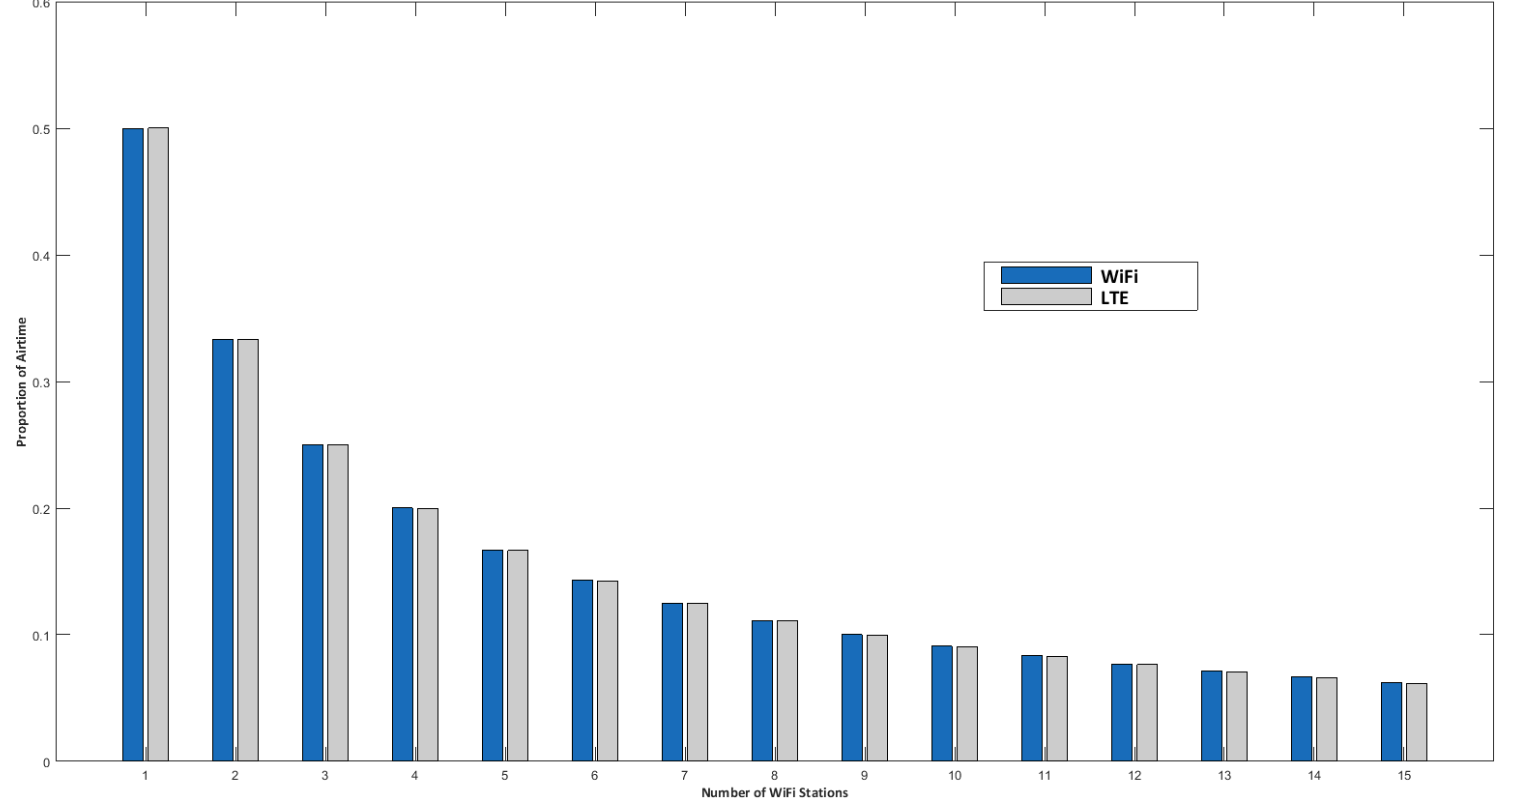
\includegraphics[width=\textwidth]{figures3/NALT-1-15}
	\caption{Airtime allocations for each station with LAA-LTE using NALT.}
	\label{basic-results}
\end{figure}
In each configuration, fair sharing was achieved, with every member of each class receiving a proportional airtime allocation. 

For comparison, the simulation was run with the same parameters as in Table \ref{params}, but with a fixed contention window size of $16$, corresponding to the midpoint of possible values under ETSI LBE LBT \cite{3gpp}. The resulting airtime allocations, normalized to the number of devices, are shown in Fig. \ref{compresults}.
\begin{figure}[!ht]
	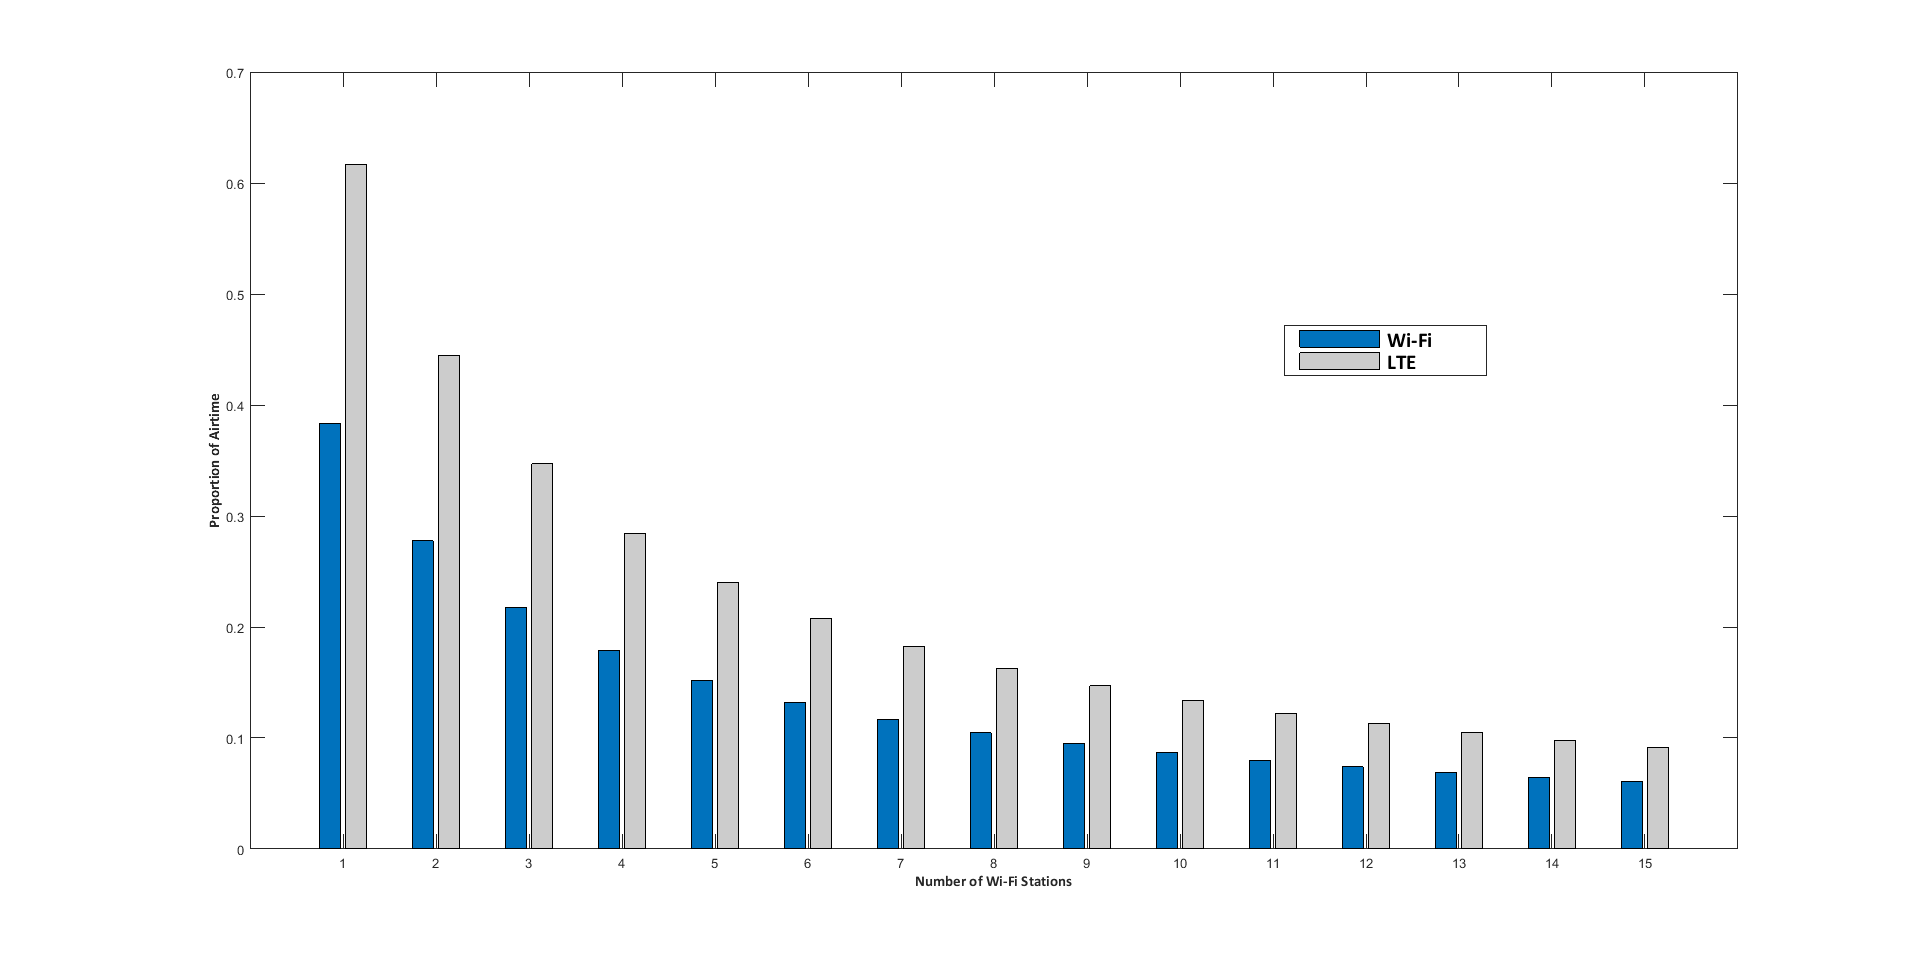
\includegraphics[width=\textwidth]{figures3/ETSIforComp}
	\caption{Airtime allocations for each station with LAA-LTE using ETSI LBE LBT.}
	\label{compresults}
\end{figure}
As expected, LAA-LTE transmission receive a disproportionately high airtime allocation as a result of the static contention window providing an increasingly higher proportion of channel accesses, when compared to Wi-Fi, as collisions on the channel occur.

Since it is likely that LAA-LTE networks will be deployed alongside other competing LAA-LTE networks, the simulation was extended to evaluate the effectiveness of NALT under these conditions.  The simulation was run with 5 independent NALT-enabled LAA-LTE networks competing against each other as well as Wi-Fi stations.  The resulting proportion of airtime for each device when using NALT is shown in Fig. \ref{multi-results}.
\begin{figure}[H]	
	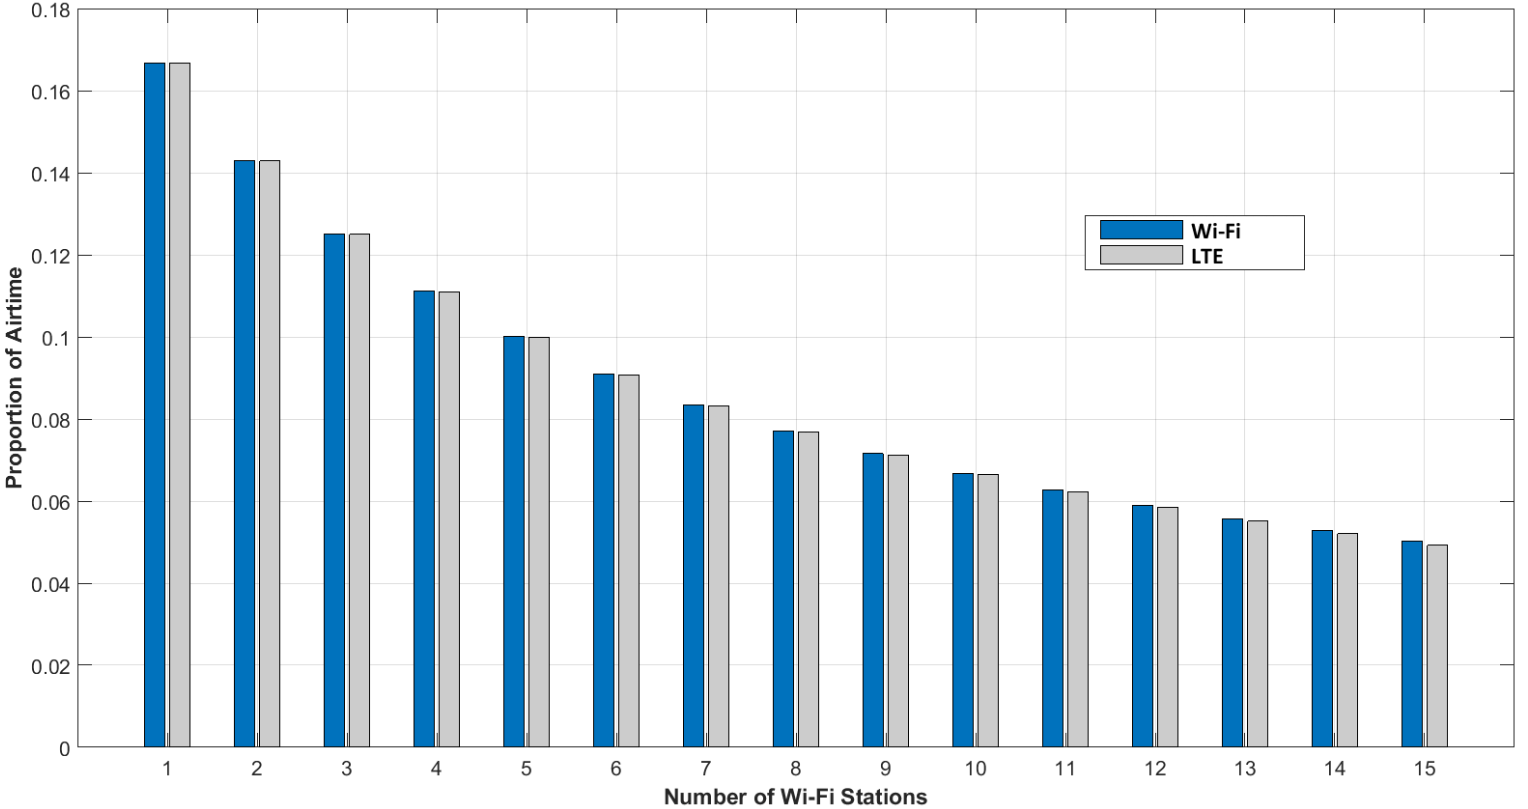
\includegraphics[width=\textwidth]{figures3/NALT-5-15}
	\caption{Airtime allocations for each station with five LAA-LTE networks using NALT.}
	\label{multi-results}
\end{figure}

If it further conceivable that LAA-LTE networks will be deployed where there are either no competing Wi-Fi stations, or the level of interference between the RATs is negligible.  Fig. \ref{NALT-only-results}, shows the resulting fair allocation of airtime for each device when NALT is used in a LAA-LTE only deployment. 
\begin{figure}[H]
	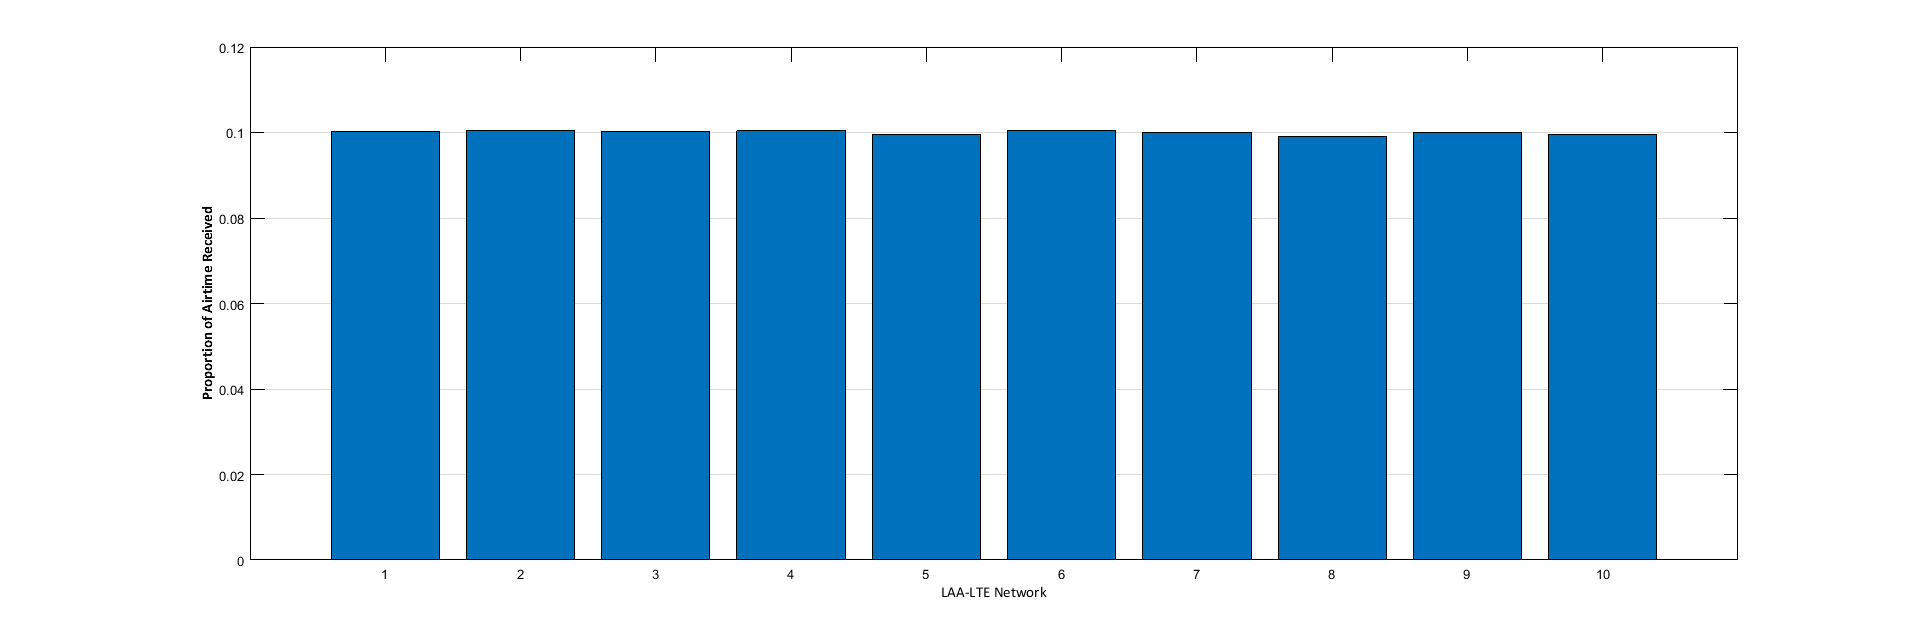
\includegraphics[width=\textwidth]{figures3/LAAonly}
	\caption{Airtime allocations from LAA-LTE only channel contention when using NALT.}
	\label{NALT-only-results}%TODO: New figure
\end{figure}

\section{Discussion and Future Work}
\label{future-work}
NALT requires no changes to \mbox{Wi-Fi} devices and in high-level simulations it shows promise in providing fair coexistence in several deployment scenarios.  In each of cases examined, NALT provides approximately equal airtime to each station, regardless of type or how many competing stations exist.  

As noted, several simplifying assumptions were made which may affect the results.  It is reasonable that \mbox{LAA-LTE} would be able to analyze the channel and determine the number or competing \mbox{Wi-Fi} stations as well as their transmission profiles, from the \mbox{Wi-Fi} preamble and MAC header, however a learning period to gather sufficient data to make reasonable estimates of the averages may or may not be necessary.  If necessary, it would negatively impact overall performance.  The assumption was made that all \mbox{Wi-Fi} stations were using the same data rate, which should provide the same results as an average data rate, but the impact on individual \mbox{Wi-Fi} stations utilizing the channel access opportunities in a multi-rate environment have not explored.  It is desirable to implement the learning functions depicted in Fig. \ref{NALT-flowchart} and determine if the processing overhead could reasonably meet the timing constraints. Further, the impacts of hidden terminals, non-saturated stations, and lossy channels, were not explored, and may have interesting implications. 

%%%%%%%%%%%%%%%%%%%%%%%% referenc.tex %%%%%%%%%%%%%%%%%%%%%%%%%%%%%%
% sample references
% %
% Use this file as a template for your own input.
%
%%%%%%%%%%%%%%%%%%%%%%%% Springer-Verlag %%%%%%%%%%%%%%%%%%%%%%%%%%

\begin{thebibliography}{99.}%
	\bibitem{3gpp}{3GPP}, ``Feasibility study on licensed-assisted access to unlicensed spectrum,'' \emph{{TR 36.889 v13.0.0}}, July 2015.
	\bibitem{chou} C.~T. Chou, K.~G. Shin, and S.~Shankar, ``{Contention-based airtime usage control in multirate IEEE 802.11 wireless LANs},'' \emph{{IEEE/ACM Transactions on Networking}}, vol.~14, no.~6, pp. 1179--1192, December 2006.	
	\bibitem{80211}``{IEEE Standard for information technology--Telecommunications and information exchange between systems Local and metropolitan area networks--Specific requirements Part 11: Wireless LAN medium access control (MAC) and physical layer (PHY) specifications},'' \emph{{IEEE Std 802.11-2012 (Revision of IEEE Std 802.11-2007)}}, pp. 818--972, March 2012.	
	\bibitem{vu} H.~L. Vu and T.~Sakurai, ``{Collision probability in saturated IEEE 802.11 networks},'' in \emph{{Australian Telecommunication Networks \& Applications Conference}}, September 2006, pp. 1--5.
	\bibitem{yoon} {J. Yoon, S. Yun, et al}, ``{Maximizing differentiated throughput in IEEE 802.11e wireless LANs},'' in \emph{{ Proceedings of the 31st IEEE Conference on Local Computer Networks}}, vol.~14, no.~6, November 2006, pp. 411--417.
\end{thebibliography}



%%%%%%%%%%%%%%%%%%%%% chapter.tex %%%%%%%%%%%%%%%%%%%%%%%%%%%%%%%%%
%
% sample chapter
%
% Use this file as a template for your own input.
%
%%%%%%%%%%%%%%%%%%%%%%%% Springer-Verlag %%%%%%%%%%%%%%%%%%%%%%%%%%
%\motto{Use the template \emph{chapter.tex} to style the various elements of your chapter content.}
\chapter{Open Questions and Potential Research Directions}
\label{open-research} % Always give a unique label
% use \chaptermark{}
% to alter or adjust the chapter heading in the running head

%\abstract*{Each chapter should be preceded by an abstract (10--15 lines long) that summarizes the content. The abstract will appear \textit{online} at \url{www.SpringerLink.com} and be available with unrestricted access. This allows unregistered users to read the abstract as a teaser for the complete chapter. As a general rule the abstracts will not appear in the printed version of your book unless it is the style of your particular book or that of the series to which your book belongs.
%Please use the 'starred' version of the new Springer \texttt{abstract} command for typesetting the text of the online abstracts (cf. source file of this chapter template \texttt{abstract}) and include them with the source files of your manuscript. Use the plain \texttt{abstract} command if the abstract is also to appear in the printed version of the book.}

%TODO: Abstract
\abstract{Each chapter should be preceded by an abstract (10--15 lines long) that summarizes the content. The abstract will appear \textit{online} at \url{www.SpringerLink.com} and be available with unrestricted access. This allows unregistered users to read the abstract as a teaser for the complete chapter. As a general rule the abstracts will not appear in the printed version of your book unless it is the style of your particular book or that of the series to which your book belongs.\newline\indent
Please use the 'starred' version of the new Springer \texttt{abstract} command for typesetting the text of the online abstracts (cf. source file of this chapter template \texttt{abstract}) and include them with the source files of your manuscript. Use the plain \texttt{abstract} command if the abstract is also to appear in the printed version of the book.}


\section{LTE-U-aware CSMA-CA and LTE-U with LBT}
\label{subsection:LTE-U-aware}

LTE-U mostly assumes neither coordination nor synchronization between itself and Wi-Fi system. LTE-U's ``on'' and ``off'' cycles are only known by LTE devices themselves. Vice versa, Wi-Fi control and management frames are known by Wi-Fi devices themselves. This independent operation results in various transmission issues. \textit{First}, in cases when LTE-U's ``on'' duration is not sufficiently long while Wi-Fi exponential back-off procedure generates long back-off intervals, Wi-Fi STAs may not have a chance to utilize the channel when LTE-U is not active. Such a conservative channel access principle wastes the radio resources and results in Wi-Fi's poor performance. \textit{Second}, an unfinished Wi-Fi frame transmission that was started during the LTE-U's ``off'' duration might be corrupted by the LTE frames once LTE switches to ``on'' cycle. Fig. \ref{figs:LTE-U-enhancement1} visualizes two examples.

To mitigate these issues, inter-RAT communications between LTE and Wi-Fi could be employed to inform Wi-Fi system the LTE-U's ``on'' and ``off'' cycles. Wi-Fi system then can adapt its MAC protocol (i) to occupy the channel more opportunistically during LTE-U's ``off'' period (but not to increase the collision probability among Wi-Fi STAs) and (ii) to schedule frame transmissions in such a way that they will not step on the next LTE-U's ``on'' cycle. Besides, frame collisions could be mitigated by incorporating some form of LBT/CCA into LTE-U. Specifically, CCA should be performed before activating LTE-U's ``on'' cycle. If the channel is detected busy, LTE-U's ``on'' cycle is deferred.

\begin{figure}[!t]
	\centering
	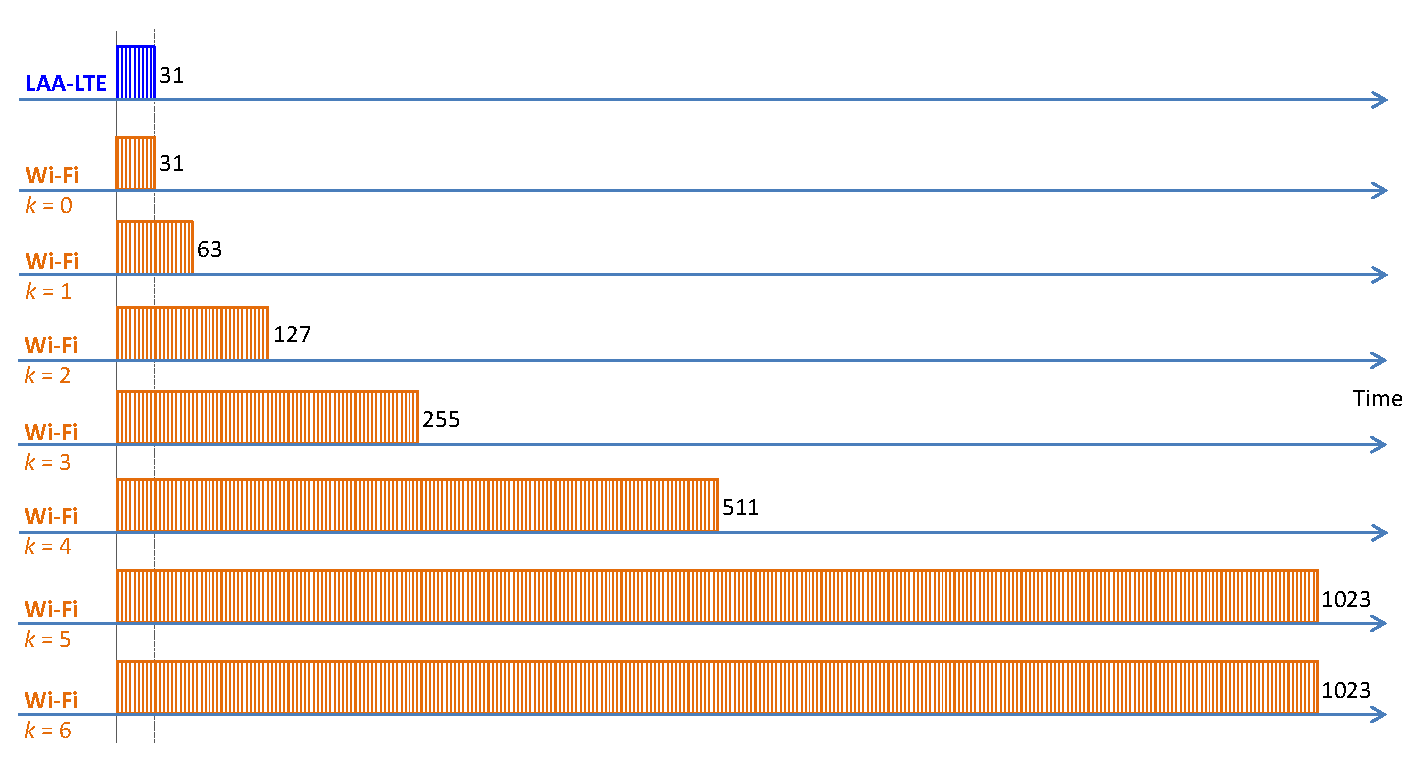
\includegraphics[width=1.0\columnwidth]{figures2/LAA-LTE-enhacement-back-off}
	\caption{Wi-Fi exponential back-off competes for the channel more conservatively, compared to LAA-LTE.}
	\label{figs:LAA-LTE-enhacement-back-off}
\end{figure}

\section{LAA-LTE with Exponential Back-off}
\label{subsection:exp-back-off}

While LBT, as a general approach, can be a good basis for coexistence of LAA-LTE and Wi-Fi, the LBE LBT in its current form (as introduced by European regulations) which is adopted for LAA-LTE is still unfair to Wi-Fi. LAA-LTE nodes impact Wi-Fi nodes in terms collision rate and probability of successful channel access more than similar Wi-Fi nodes on the same carrier. This is not compliant with the objectives as listed in 3GPP LAA LTE Study Item \cite{LAA-LTE-SI}: ``LAA should not impact Wi-Fi services (data, video and voice services) more than an additional Wi-Fi network on the same carrier; these metrics could include throughput, latency, jitter, etc.''. One major and obvious reason is, that while Wi-Fi applies exponential back-off rule, LAA-LTE simply applies fixed-size back-off rule. In order to elaborate this observation, consider a typical example follows. It is assumed that $W^{\mathrm{LAA-LTE}}=31$, $W^{Wi-Fi}_{\min}=31$, and $W^{\mathrm{Wi-Fi}}_{\max}=1023$. Then, as descirbed in subsection \ref{subsection:LAA-LTE}, LTE-U always back-offs with contention window $W^{\mathrm{LAA-LTE}}=31$. For Wi-Fi, as descirbed in subsection \ref{subsubsection:IEEE 802.11 CSMA-CA}, it back-offs with contention window $W(0)=31$ for the initial transmission attempt. However, if collisions occur, it progressibly doubles its contention windows to reduce the probability of a subsequent collision: $W(1)=63$ (the first re-transmission attempt), $W(2)=127$ (the second re-transmission attempt), $W(3)=255$ (the third re-transmission attempt), $W(4)=511$, $W(5)=1023$, $W(6)=1023$, and etc. Fig. \ref{figs:LAA-LTE-enhacement-back-off} compares contention windows of LAA-LTE and Wi-Fi.

At present, there is no existing work that studies how an exponential back-off can help to improve the fairness between LAA-LTE and Wi-Fi. It is important to note that, compared to Wi-Fi, designing an exponential back-off protocol for LAA-LTE that employs OFDMA-based MAC layer might not be straightforward. In details, Wi-Fi adopts OFDM in the PHY layer and allows only one user to occupy the whole channel at one time. Its contention window is scaled respectively to the outcome (success or failure) of a frame transmission to given user. For LTE, OFDMA devides the system bandwidth into a series of Physical Resource Blocks (PRBs). Each PRB is composed of $12$ OFDM subcarriers. Different PRBs can be allocated to different users in a given subframe and multiple users can occupy the channel at the same time. This implies that the rule governing the adaptation of contention window of LAA-LTE is required to be more sophisticated than that of Wi-Fi. In adddition to back-off procedure design, there are two other interesting questions: (i) how exponential back-off could (negatively) affect the performance and efficiency of LAA-LTE; and (ii) what could be appropriate values for LAA-LTE's operation parameters.

A side note is that, according to \cite{U-LTE-FCC-Cisco-2015}, 3GPP is now having a working agreement to use a LBT mechanism with exponential back-off. At this moment, LAA-LTE standard is not yet finalized by 3GPP and no information is publicly available. ETSI is also devising a set of minimum ``fairness'' requirements as part of EN 301 893 standard for ``5 GHz high performance wireless access systems'' in Europe (scheduled to be completed by the end of 2015).
\begin{figure}[!t]
	\centering
	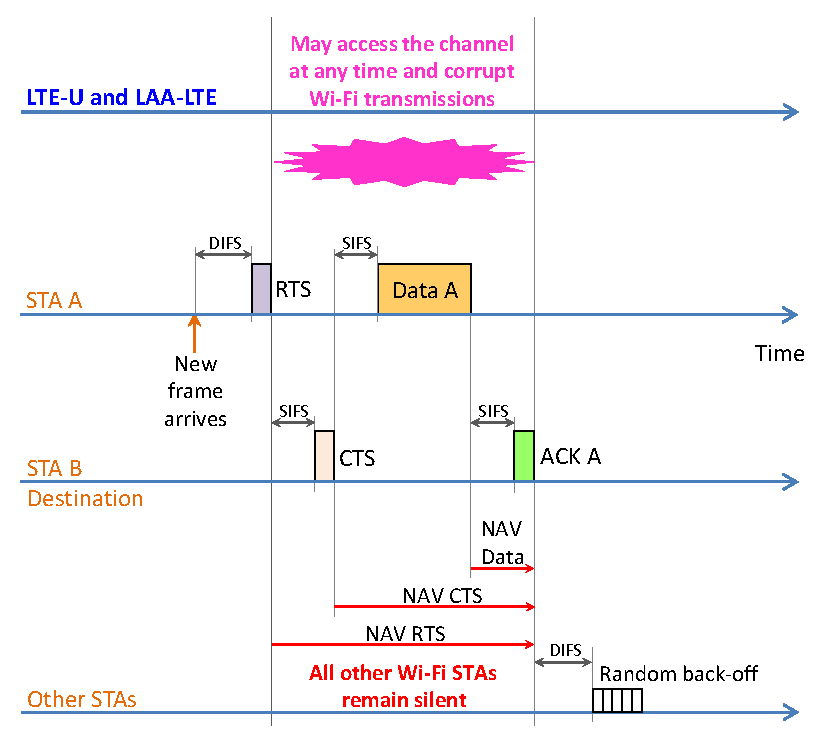
\includegraphics[width=0.7\columnwidth]{figures2/LTE-U-enhancement-RTS-CTS-NAV}
	\caption{U-LTE may cause channel collisions with Wi-Fi at any time.}
	\label{figs:LTE-U-enhancement-RTS-CTS-NAV}
\end{figure}

\section{Wi-Fi-aware LTE-U and LAA-LTE}
\label{subsection:Wi-Fi-aware}

As addressed in subsection \ref{subsubsection:IEEE 802.11 CSMA-CA}, RTS/CTS and NAV are effective and important mechanisms employed by the IEEE 802.11 CSMA-CA protocol to reserve the channel and avoid collisions. However, since U-LTE and Wi-Fi are not collaborating, Wi-Fi's NAV information carried by RTS, CTS, and data frames is not known by U-LTE devices. In other words, while Wi-Fi STAs defer their transmissions until ongoing frame exchanges are done, U-LTE devices do not respect Wi-Fi reservation and may start their transmissions at any time, as shown in Fig. \ref{figs:LTE-U-enhancement-RTS-CTS-NAV}. This may result in a high rate of channel collisions and corrupt both Wi-Fi and U-LTE transmissions. As visualized Fig. \ref{figs:LTE-U-enhancement-RTS-CTS-NAV}, an U-LTE transmission could accidentally destroy the whole Wi-Fi transmission session composing of RTS, CTS, data, and ACK frames (at the same time, U-LTE frame is also corrupted by Wi-Fi frames). Mechanisms that provide U-LTE with information on Wi-Fi activities to avoid such transmission corruptions could be therefore very beneficial.

\section{Collaborative U-LTE and Wi-Fi}
As metioned so far, almost all existing works dealing with U-LTE and Wi-Fi coexistence assume non-cooperative approach which does not required any information exchange between these two networks. LTE is simply additionally equipped with some mechanisms to friendly share the same channel with existing Wi-Fi networks. The authors in \cite{U-LTE-5G-2015, Coordinated-LTE-U-Wi-Fi-2015} carry out preliminiary investigations towards this direction. However, only conceptual network archirectures and mechanisms and are presented. Collaborative approaches is quite interesting since it may result in better coexistence by sharing information between different radio access technologies (RATs) and enabling global/local optimizations. Some benefits of such approaches has been outlined in subsections \ref{subsection:LTE-U-aware} and \ref{subsection:Wi-Fi-aware}. This approach, on the other hand, may be challenging since it needs additional network infrastructure/entities and set of protocols for inter-RAT communications. They are required for discovery of neighboring radio systems, selecting operating channels/transmission power, etc., for radio systems, and providing some level of fair and/or efficient use of available channels. 

\section{Inter-operator U-LTE Coexistence}
In addition to coexistence between U-LTE and Wi-Fi, coexistence among U-LTE systems deployed by different operators running in a shared band is also a critical concern. This concern is more pronounced in high density urban areas with a very large number of devices/system running different protocols. Work in \cite{LTE-U-ICC-WS-2015} presents a preliminary study on this and the results show that LBT mechanisms can increase the network throughput since collisions can be mitigated. Work in \cite{Enhanced-LTE-U-thesis-2015} investigates the interactions between different LBT mechanisms when they are deployed in proximity of each other. Inter-operator U-LTE coexistence is especially important when multiple operators employ similar MAC protocols based on fixed contention windows that could be accidentally synchronized in channel access attemps and result in consecutive collisions. As a result, exponential back-off rules, inter-RAT communications, and collaborative inteference management protocols could be promising approaches.

\section{Other Considerations on Coexistence}
Operations, system performance, and coexistence of radio networks highly depend on deployment scenarios. This is the main reason why a number of existing work supports U-LTE technology while the others call for further investigations and developments before deploying this technology. Also, different coexistence mechanisms are recommended for different scenarios. For a complete understanding of U-LTE impacts on Wi-Fi, a wide range of node and load densities should be considered. Besides, performance of voice and video-related applications should be evaluated. For most of existing work, only throughput and channel access probability of Wi-Fi networks are evaluated. However, an insight to latency and jitter performance could be desirable. Besides, it would be interesting to take into account the operations and performance of recent Wi-Fi variants when coexisting with U-LTE.

\section{Emerging Wi-Fi Technologies and U-LTE}
With the currrent trends of future RANs including network densification, heterogeneous network (HetNet), Internet of Things (IoT), the explosion of various applications (smart homes/cities, smart transportations, automomous vehicles, etc.), and etc., numberous technological evolutions have been expecting. For time-sensitive applications (e.g., sensor and control for critical infrastructures and automomous vehicles), data communications is required to be extremely reliable, robust, energy-efficient while being able to guaratee latencies in millisecond or sub-millisecond scale. These requirements urge for the developments of collaborative, well-controlled, and synchronous Wi-Fi MAC protocols (instead of distributed, random-access-based, and asynchronous IEEE 802.11 CSMA/CA that have been widely deployed). To this end, PCF and HCCA operation schemes (specified in IEEE 802.11/802.11e standards but not widely used) should be re-visited.

Despite the fact that PCF and HCCA allocate the channel to STAs in a well-controlled manner, their performance (in terms of throughput, latency, and power consumption) is still questionable due to their complexities and signaling overheads, specially in highly dense networks with a vast number of battery-operated devices exchanging short and bursty messages. Furthermore, it is compelling to understand their interaction and coexistence with U-LTE. While CFP and CAP are desired for time-sensitive applications, the aggressive operation of U-LTE in the same frequency band may render them impossible. Finally, protocols and enabling technologies for collaborations and synchronizations between PCF-/HCCA-based Wi-Fi and U-LTE appear to be essential and thus could be very interesting working areas.

%%%%%%%%%%%%%%%%%%%%%%%% referenc.tex %%%%%%%%%%%%%%%%%%%%%%%%%%%%%%
% sample references
% %
% Use this file as a template for your own input.
%
%%%%%%%%%%%%%%%%%%%%%%%% Springer-Verlag %%%%%%%%%%%%%%%%%%%%%%%%%%
%

\begin{thebibliography}{99.}%
\bibitem{LAA-LTE-SI}``{3GPP™} work item: Study on licensed-assisted access using {LTE} to unlicensed spectrum,'' 3rd Generation Partnership Project (3GPP).

\bibitem{U-LTE-FCC-Cisco-2015}M.~L. Brown, ``Current trends in {LTE-U} and {LAA} technology,'' Comments of Qualcomm Incoporated, Qualcomm Inc., Jun. 2015.

\bibitem{U-LTE-5G-2015}
A.~Al-Dulaimi, S.~Al-Rubaye, Q.~Ni, and E.~Sousa, ``{5G} communications race:Pursuit of more capacity triggers {LTE} in unlicensed band,'' \emph{IEEE Vehicular Technology Magazine}, vol.~10, no.~1, pp. 43--51, March 2015.

\bibitem{Coordinated-LTE-U-Wi-Fi-2015} S.~Sagari, S.~Baysting, D.~Saha, I.~Seskar, W.~Trappe, and D.~Raychaudhuri,``Coordinated dynamic spectrum management of {LTE-U} and {Wi-Fi} networks,''
in \emph{2015 IEEE International Symposium on Dynamic Spectrum Access Networks (DySPAN)}, Sept 2015, pp. 209--220.

\bibitem{LTE-U-ICC-WS-2015}A.~Voicu, L.~Simic, and M.~Petrova, ``Coexistence of pico- and femto-cellular {LTE}-unlicensed with legacy indoor {Wi-Fi} deployments,'' in \emph{2015 IEEE	International Conference on Communication Workshop (ICCW)}, June 2015, pp.2294--2300.

\bibitem{Enhanced-LTE-U-thesis-2015}A.~Kanyeshuli, ``{LTE} in unlicensed band: Medium access and performance evaluation,'' Master's thesis, University of Agder, Norway, May 2015.
\end{thebibliography}

%%%%%%%%%%%%%%%%%%%%%% appendix.tex %%%%%%%%%%%%%%%%%%%%%%%%%%%%%%%%%
%
% sample appendix
%
% Use this file as a template for your own input.
%
%%%%%%%%%%%%%%%%%%%%%%%% Springer-Verlag %%%%%%%%%%%%%%%%%%%%%%%%%%

\appendix
\motto{All's well that ends well}
\chapter{Chapter Heading}
\label{introA} % Always give a unique label
% use \chaptermark{}
% to alter or adjust the chapter heading in the running head

Use the template \emph{appendix.tex} together with the Springer document class SVMono (monograph-type books) or SVMult (edited books) to style appendix of your book in the Springer layout.


\section{Section Heading}
\label{sec:A1}
% Always give a unique label
% and use \ref{<label>} for cross-references
% and \cite{<label>} for bibliographic references
% use \sectionmark{}
% to alter or adjust the section heading in the running head
Instead of simply listing headings of different levels we recommend to let every heading be followed by at least a short passage of text. Furtheron please use the \LaTeX\ automatism for all your cross-references and citations.


\subsection{Subsection Heading}
\label{sec:A2}
Instead of simply listing headings of different levels we recommend to let every heading be followed by at least a short passage of text. Furtheron please use the \LaTeX\ automatism for all your cross-references and citations as has already been described in Sect.~\ref{sec:A1}.

For multiline equations we recommend to use the \verb|eqnarray| environment.
\begin{eqnarray}
\vec{a}\times\vec{b}=\vec{c} \nonumber\\
\vec{a}\times\vec{b}=\vec{c}
\label{eq:A01}
\end{eqnarray}

\subsubsection{Subsubsection Heading}
Instead of simply listing headings of different levels we recommend to let every heading be followed by at least a short passage of text. Furtheron please use the \LaTeX\ automatism for all your cross-references and citations as has already been described in Sect.~\ref{sec:A2}.

Please note that the first line of text that follows a heading is not indented, whereas the first lines of all subsequent paragraphs are.

% For figures use
%
\begin{figure}[t]
\sidecaption[t]
%\centering
% Use the relevant command for your figure-insertion program
% to insert the figure file.
% For example, with the option graphics use
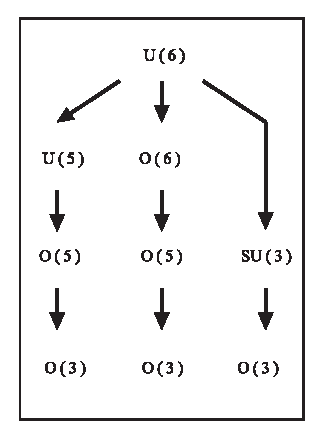
\includegraphics[scale=.65]{figure}
%
% If not, use
%\picplace{5cm}{2cm} % Give the correct figure height and width in cm
%
\caption{Please write your figure caption here}
\label{fig:A1}       % Give a unique label
\end{figure}

% For tables use
%
\begin{table}
\caption{Please write your table caption here}
\label{tab:A1}       % Give a unique label
%
% For LaTeX tables use
%
\begin{tabular}{p{2cm}p{2.4cm}p{2cm}p{4.9cm}}
\hline\noalign{\smallskip}
Classes & Subclass & Length & Action Mechanism  \\
\noalign{\smallskip}\hline\noalign{\smallskip}
Translation & mRNA$^a$  & 22 (19--25) & Translation repression, mRNA cleavage\\
Translation & mRNA cleavage & 21 & mRNA cleavage\\
Translation & mRNA  & 21--22 & mRNA cleavage\\
Translation & mRNA  & 24--26 & Histone and DNA Modification\\
\noalign{\smallskip}\hline\noalign{\smallskip}
\end{tabular}
$^a$ Table foot note (with superscript)
\end{table}
%


%\backmatter%%%%%%%%%%%%%%%%%%%%%%%%%%%%%%%%%%%%%%%%%%%%%%%%%%%%%%%
%%%%%%%%%%%%%%%%%%%%%%%acronym.tex%%%%%%%%%%%%%%%%%%%%%%%%%%%%%%%%%%%%%%%%%
% sample list of acronyms
%
% Use this file as a template for your own input.
%
%%%%%%%%%%%%%%%%%%%%%%%% Springer %%%%%%%%%%%%%%%%%%%%%%%%%%

\Extrachap{Glossary}


Use the template \emph{glossary.tex} together with the Springer document class SVMono (monograph-type books) or SVMult (edited books) to style your glossary\index{glossary} in the Springer layout.


\runinhead{glossary term} Write here the description of the glossary term. Write here the description of the glossary term. Write here the description of the glossary term.

\runinhead{glossary term} Write here the description of the glossary term. Write here the description of the glossary term. Write here the description of the glossary term.

\runinhead{glossary term} Write here the description of the glossary term. Write here the description of the glossary term. Write here the description of the glossary term.

\runinhead{glossary term} Write here the description of the glossary term. Write here the description of the glossary term. Write here the description of the glossary term.

\runinhead{glossary term} Write here the description of the glossary term. Write here the description of the glossary term. Write here the description of the glossary term.
%
\Extrachap{Solutions}

\section*{Problems of Chapter~\ref{intro}}

\begin{sol}{prob1}
The solution\index{problems}\index{solutions} is revealed here.
\end{sol}


\begin{sol}{prob2}
\textbf{Problem Heading}\\
(a) The solution of first part is revealed here.\\
(b) The solution of second part is revealed here.
\end{sol}


%\printindex

%%%%%%%%%%%%%%%%%%%%%%%%%%%%%%%%%%%%%%%%%%%%%%%%%%%%%%%%%%%%%%%%%%%%%%
%TODO: Complete acronyms (either more definitions, or none: the SG book had none, the spring latex file indicated they maybe should have some
%TODO: QDH update/edit sections per prof comments
%TODO: Validate that figures are still meaningful and clear in black & white (greyscale?)
%TODO: Full read-through edit
%TODO: Add conclusion chapter ?
%TODO: Remove abstract label from chapters per prof, but retain the content in the latex file with the \abstract* tag as this will be extracted by Spring for the online listings
\end{document}